\documentclass[a4paper,twocolumn]{report}

% some definitions for the title page
\newcommand{\reporttitle}{Cost-opportunistic data processing in serverless environments}
\newcommand{\reportauthor}{Oli Callaghan (oe119@ic.ac.uk) [01508136]}
\newcommand{\supervisor}{Dr Holger Pirk}
\newcommand{\reporttype}{MEng Individual Project}
\newcommand{\degreetype}{MEng Computing (Artifical Intelligence and Machine Learning)}

% Define commonly used terms
\newcommand{\faas}{FaaS}
\newcommand{\faaslong}{Functions-as-a-Service}
\newcommand{\faasxlong}{\faaslong{} (\faas{})}

% Define commonly used terms relating to serverless
\newcommand{\awslambda}{AWS Lambda}

% Define commonly used terms relating to the project
\newcommand{\faaasc}{\texttt{faaasc}}

% load required packages
\usepackage[a4paper,hmargin=2.8cm,vmargin=2.0cm,includeheadfoot]{geometry}
\usepackage{textpos} % positioning
\usepackage{biblatex} % bibliography
\usepackage{tabularx,longtable,multirow,subfigure,caption} % hangcaption
\usepackage{fncylab} % formatting of labels
\usepackage{fancyhdr} % page layout
\usepackage{url} % URLs
\usepackage[english]{babel} % for internalisation
\usepackage{amsmath} % for mathematical formulae
\usepackage{dsfont} % for mathematical symbols
\usepackage{epstopdf} % automatically replace .eps with .pdf in graphics
\usepackage{array} % tables
\usepackage{latexsym} % symbols

\usepackage{subcaption} % For subfigures

% Because of the way minted works, it needs to be loaded before hyperref
\usepackage[pdftex,hypertexnames=false,colorlinks]{hyperref} % provide links in pdf

% For code listings
\usepackage{listings}
\usepackage{minted}

\usepackage{todonotes} % Because you're a lazy bastard
\usepackage{csquotes} % Not sure what this is for
\usepackage{siunitx} % For SI units

% For generated diagrams and plots
\usepackage{graphicx}
\usepackage{layouts}
\usepackage{lmodern}
\usepackage{tikz}
\usepackage{tikz-cd}
\usepackage{pgfplots}

\setminted{linenos}
\setminted{breaklines}
\setminted{xleftmargin=24pt}

\hypersetup{pdftitle={},
  pdfsubject={},
  pdfauthor={},
  pdfkeywords={},
  pdfstartview=FitH,
  pdfpagemode={UseOutlines},% None, FullScreen, UseOutlines
  bookmarksnumbered=true, bookmarksopen=true, colorlinks,
    citecolor=black,%
    filecolor=black,%
    linkcolor=black,%
    urlcolor=black}

\usepackage[all]{hypcap}

%%% Default fonts
\renewcommand*{\rmdefault}{bch}
\renewcommand*{\ttdefault}{cmtt}

%%% Default settings (page layout)
\setlength{\parindent}{0em} % indentation of paragraph

\setlength{\parindent}{0em} % indentation of paragraph

\setlength{\headheight}{14.5pt}
\pagestyle{fancy}
\renewcommand{\chaptermark}[1]{\markboth{\chaptername\ \thechapter.\ #1}{}}

\fancyfoot[ER,OL]{\thepage} % page no. in the left on odd pages and on right on even pages
\fancyfoot[OC,EC]{\sffamily }
\renewcommand{\headrulewidth}{0.1pt}
\renewcommand{\footrulewidth}{0.1pt}
\captionsetup{margin=10pt,font=small,labelfont=bf}

%--- chapter heading
\def\@makechapterhead#1{%
  \vspace*{10\p@}%
  {\parindent \z@ \raggedright \sffamily
    \interlinepenalty\@M
    \Huge\bfseries \thechapter \space\space #1\par\nobreak
    \vskip 30\p@
  }}

%--- chapter heading
\def\@makechapterhead#1{%
  \vspace*{10\p@}%
  {\parindent \z@ \raggedright \sffamily
        %{\Large \MakeUppercase{\@chapapp} \space \thechapter}
        %\\
        %\hrulefill
        %\par\nobreak
        %\vskip 10\p@
    \interlinepenalty\@M
    \Huge\bfseries \thechapter \space\space #1\par\nobreak
    \vskip 30\p@
  }}

%---chapter heading for \chapter*
\def\@makeschapterhead#1{%
  \vspace*{10\p@}%
  {\parindent \z@ \raggedright
    \sffamily
    \interlinepenalty\@M
    \Huge \bfseries  #1\par\nobreak
    \vskip 30\p@
  }}
\allowdisplaybreaks

% Matplotlib required preamble
\def\mathdefault#1{#1}
\everymath=\expandafter{\the\everymath\displaystyle}
\makeatletter\@ifpackageloaded{underscore}{}{\usepackage[strings]{underscore}}\makeatother


% load references for bibliography
\addbibresource{references.bib}

% load the title page
\begin{document}
% Last modification: 2015-08-17 (Marc Deisenroth)
\begin{titlepage}

\newcommand{\HRule}{\rule{\linewidth}{0.5mm}} % Defines a new command for the horizontal lines, change thickness here

%----------------------------------------------------------------------------------------
%	LOGO SECTION
%----------------------------------------------------------------------------------------


\includegraphics[width = 8cm]{./assets/imperial.pdf}\\[2.5cm]

\center % Center everything on the page

%----------------------------------------------------------------------------------------
%	HEADING SECTIONS
%----------------------------------------------------------------------------------------

\textsc{\LARGE \reporttype}\\[1.5cm]
\textsc{\Large Department of Computing}\\[0.5cm]
\textsc{\large Imperial College of Science, Technology and Medicine}\\[0.5cm]

%----------------------------------------------------------------------------------------
%	TITLE SECTION
%----------------------------------------------------------------------------------------

\HRule \\[0.4cm]
{ \huge \bfseries \reporttitle}\\ % Title of your document
\HRule \\[1.5cm]

%----------------------------------------------------------------------------------------
%	AUTHOR SECTION
%----------------------------------------------------------------------------------------

\begin{minipage}{0.4\textwidth}
\begin{flushleft} \large
\emph{Author:}\\
\reportauthor % Your name
\end{flushleft}
\end{minipage}
~
\begin{minipage}{0.4\textwidth}
\begin{flushright} \large
\emph{Supervisor:} \\
\supervisor % Supervisor's Name
\end{flushright}
\end{minipage}\\[4cm]




%----------------------------------------------------------------------------------------


%----------------------------------------------------------------------------------------
%	DATE SECTION
%----------------------------------------------------------------------------------------

{\large \today} % Date, change the \today to a set date if you want to be precise


\vfill % Fill the rest of the page with whitespace
Submitted in partial fulfillment of the requirements for the \degreetype~of Imperial College London

\end{titlepage}


% page numbering etc.
\pagenumbering{roman}
\clearpage{\pagestyle{empty}\cleardoublepage}
\setcounter{page}{1}
\pagestyle{fancy}

\begin{abstract}
This research aims to address a critical billing inefficiency in \faasxlong{} environments, whereby \faas{} functions are charged for allocated resources and execution time whilst awaiting I/O operations, such as network requests. Through developing a novel serverless runtime, this research intends to allow function invocations to release unused allocated resources back to the runtime such to be reallocated to other functions, and more accurately billing \faas{} functions for their actual usage.
\end{abstract}


\cleardoublepage
\section*{Acknowledgments}
Comment this out if not needed.


\clearpage{\pagestyle{empty}\cleardoublepage}

% Table of Contents
\fancyhead[RE,LO]{\sffamily {Table of Contents}}
\tableofcontents

\clearpage{\pagestyle{empty}\cleardoublepage}
\pagenumbering{arabic}
\setcounter{page}{1}
\fancyhead[LE,RO]{\slshape \rightmark}
\fancyhead[LO,RE]{\slshape \leftmark}

% Introduction
\chapter{Introduction}

\begin{figure}
    \begin{center}
        \input{node_modules/@faaas/perf-v8-event-loop-results/assets/faas-profile-waiting-on-io.pgf}
    \end{center}
    \caption{Profile of a four CRUD \faas{} functions querying a PostgreSQL database with simulated additional latency. Time is broken down by phase, covering time spent in the kernel during syscalls, executing NodeJS code, and blocked on IO.}
    \label{fig:faas-profile-intro-experiment}
\end{figure}

\faasxlong{} provides an abstraction over application development, decomposing programs into isolated stateless units called `functions', invoked by events such as HTTP requests, or messages received from a message bus\cite{ibmWhatFaaSFunctionasaService2024}.

This abstraction simplifies development, allowing developers to focus on the underlying business logic of their system, rather than managing and scaling infrastructure. Typically, developers design serverless functions to be stateless\cite{ggailey777AzureFunctionsBest2022}, enabling horizontal scaling\cite{ngoEvaluatingScalabilityElasticity2022}, communicating with persistent storage to persist state between function invocations.

In these execution environments, whilst `functions' are running, they are allocated, guaranteed and billed for resources such as CPU and memory throughout the lifecycle of its invocation. Whilst in theory this seems beneficial, in practice, this leads to wasted resources, as the function may be awaiting an asynchronous operation to complete, such as a network request. This research seeks to reduce this wastage.

In these environments, `functions' are typically implemented either as containers or as virtual machines running atop a serverless `runtime'; whilst these containers are awaiting I/O such as network requests, resources are still allocated, used to determine whether execution can continue.

\section{Motivation}
% Syscall Calls Breakdown
\begin{figure}
    \begin{center}
        \input{node_modules/@faaas/perf-v8-event-loop-results/assets/faas-profile-strace-calls.pgf}
    \end{center}
    \caption{\texttt{strace} profile of the \faas{} petstore, showing the frequency of calls to each syscall during the course of the experiement.}
    \label{fig:faas-strace-freq-intro-experiment}
\end{figure}

% Syscall Time Breakdown
\begin{figure}
    \begin{center}
        \input{node_modules/@faaas/perf-v8-event-loop-results/assets/faas-profile-strace-time.pgf}
    \end{center}
    \caption{\texttt{strace} profile of the \faas{} petstore, showing the time spent in each of the syscalls during the course of the experiement.}
    \label{fig:faas-strace-time-intro-experiment}
\end{figure}

Typical \faas{} workloads can be characterised as `glue', most commonly handling HTTP requests and interacting with a form of persistent storage --- in fact, around 50\% of all serverless functions fall into this category\cite{eismannReviewServerlessUse2020}.

\faas{} architectures generally tend to decrease costs, achieving this by using a fine-grained billing model as described in Section \ref{sec:faas-billing-models}, charging per invocation, and for compute and memory allocations in subsecond increments over the duration of execution, ensuring wasted resources are released back to the cloud provider once a function terminates.

The resolution of the billing model however extends only to the level of granularity of functions, whereby resources are allocated for the entire lifetime of the function's execution. This is particularly important when considering that serverless suffers from additional latency when accessing persistent storage, for example, the average latency between AWS Lambda and DynamoDB is usually between \qtyrange{60}{90}{\ms}\cite{ghoshCachingTechniquesImprove2020}.

% PProf Sample from PetStore PutPet Function
\begin{figure*}
    \begin{center}
        \begin{tikzpicture}[scale = 0.75, every node/.style={scale=0.75}]
            \input{node_modules/@faaas/perf-v8-event-loop-results-pprof/assets/faas-profile-pprof-put-pet.pgf}
        \end{tikzpicture}
    \end{center}
    \caption{\texttt{pprof} profile of the \faas{} petstore showing where in the program wall-clock time was spent whilst in the NodeJS phase shown in Figure \ref{fig:faas-strace-freq-intro-experiment}.}
    \label{fig:faas-pprof-intro-experiment}
\end{figure*}

Since the median execution time for serverless functions lies between milliseconds and a second\cite{eismannReviewServerlessUse2020}, this latency accounts for a significant proportion of time when resources are allocated and unused during function execution time. Developers are charged for this time, and cannot temporarily yield resources back to the host until the asynchronous action completes. This is refered to as the double billing problem\cite{baldiniServerlessTrilemmaFunction2017,yuCharacterizingServerlessPlatforms2020} and discussed further in Section \ref{sec:double-billing-problem}.

\subsection{Motivational Experiment}
To demonstrate the extent of this problem, a small introductory experiment is proposed, whereby four simple CRUD \faas{} functions are executed within a sandboxed environment, allocated \SI{128}{\mega\byte} of RAM and 0.1 CPU share each, querying an SQL database that has been configured to introduce a random delay of between \qtyrange{60}{90}{\ms} to each query to simulate the typical latency of DynamoDB.

The results of profiling the time spent executing the actual underlying function compared with time the function is idle is shown in Figure \ref{fig:faas-profile-intro-experiment}. Additionally, a \verb|pprof| trace of wall clock time spent in each section of the body of the function and \verb|strace| traces identifying the most common syscalls are provided in Figures \ref{fig:faas-pprof-intro-experiment},
\ref{fig:faas-strace-freq-intro-experiment} and \ref{fig:faas-strace-time-intro-experiment}.

From the initial results, it is clear that the function spends the vast majority of its time blocked on I/O, and is unable to release resources back to the runtime. Additionally, the most frequent syscall is \verb|epoll_wait|, which yields a process back to the operating system until IO is ready, indicating that under these resources allocations, with the described latency, the function is wasting a large portion of its allocated resources idle.

\section{Contributions}

This research aims to yield control back to the runtime from these `functions' whilst awaiting asynchronous operations to complete, allowing useful work to be scheduled by the runtime in its place. Throughout this report, we propose three main contributions:

\begin{itemize}
    \item The \faaasc{} compiler that performs code splitting of JavaScript serverless functions, allowing a function to optionally be deployed in a split manner on any supported \faas{} platform (currently only AWS Lambda is supported).

    \item Adaptive function splitting strategy, which determines the probability of profitability when splitting a function, and acts accordingly.

    \item An evaluation of \faaas{} when deployed to AWS Lambda, with analysis on the impact of a set of hypothetical billing models on split functions.
\end{itemize}

\section{Thesis Structure}
This thesis is structured as follows: Chapter \ref{chap:background} provides an introduction to \faas{}, and the challenges associated with more fine-grained billing. Chapter \ref{chap:concepts} formalises a probabilistic model to allow a function to decide when to split and when not to. It also introduces the concepts related to functions returning continuations. Chapter \ref{chap:impl} details the implementation of the \faaasc{} compiler and the adaptive code splitting strategy. Chapter \ref{chap:eval} evaluates these split functions generated by \faaasc{}, and evaluates this in the context of a hypothetical billing model. Chapter \ref{chap:conclusion} concludes the thesis by discussing future work for \faaas{} in addition to highlighting the key areas that cloud providers need to address in order to apply \faaas{} split functions to OLTP workloads.

\chapter{Ethical Considerations}
Serious ethical consideration is required when designing any systems which may affect the bottom lines of highly profiable cloud providers. By allowing customers to avoid renting overpriced compute which inevitably goes unused, the cloud providers are losing out on potential revenue. How will Bezos afford his next yacht if we're not paying for our unused compute?

\chapter{Background}

\section{Terminology}
\subsection{What is serverless?}
\todo[inline]{Cite page 168 of wardley maps book}
Serverless computing emerged in the mid-to-late 2000s\cite{wardleyWardleyMaps2022,IntroducingGoogleApp,patilServerlessComputingEmergence2021} as a new paradigm for deploying applications, with the emergence of low-cost public cloud providers\cite{patilServerlessComputingEmergence2021,BenjaminBlackEC2}. It allows developers to deploy applications without managing the underlying infrastructure, leading to much more scalable and cost-effective solutions.

Typically, resources such as VMs\cite{hoeferTaxonomyCloudComputing2010} are rented in sub-second increments, and with storage and network charged by total usage. This results in a Pay-as-you-go (PAYG) model that can adapt to highly variable workloads\cite{sehgalCostBillingPractices2023,hilleyCloudComputingTaxonomy2009}.

Serverless applications are usually composed of cloud provider managed services, such as databases, storage, and compute, and are often event-driven\cite{EventarcOverview,EventListenerAmazon,robeceOverviewAzureEvent2024}. This means that application logic can be invoked by events, such as HTTP requests, database changes, or file uploads. This allows the application to scale independently\cite{goniwadaCloudNativeArchitecture2022}, as the cloud provider can provision resources as needed.

\subsection{What is a VM?}
Virtual Machines (VMs) are a form of virtualisation that enables multiple operating systems to run on a single physical host machine\cite{ramosjoaocarloscarvalhodossantosSecurityChallengesVirtualization2009}. They run ontop of a hypervisor or virtual machine monitor (VMM), and are typically used to run systems for multiple tennants on the same physical hardware. Typically VMs enable more optimal use of hardware resources \cite{desaiHypervisorSurveyConcepts2013}.

Since VMs do not share a kernel, they provide a high level of isolation between VMs\cite{hoeferTaxonomyCloudComputing2010}, whereby isolation is enforced by the VMM. This eliminates an entire set of security vulnerabilities, notabily kernel layer vulnerabilities, since for a malicious VM to access another, it must find vulnerabilities in the kernel. Whilst VMs reduce the attack surface for vulnerabilities, they do not eliminate it entirely, as there could still be vulnerabilities in the VMMs itself\cite{reubenSurveyVirtualMachine,ramosjoaocarloscarvalhodossantosSecurityChallengesVirtualization2009}.

Additionally, hypervisors tend to allocate fixed resources for the lifetime of the VM, allowing for guaranteed CPU time, memory and storage\cite{hoeferTaxonomyCloudComputing2010}, however can utilise ballooning to overprovision memory and borrow/steal this from VMs running on the hypervisor\cite{moniruzzamanAnalysisMemoryBallooning2014}. Additionally, hotplugging\cite{hildenbrandVirtiomemParavirtualizedMemory2021,LKMLDanielKiper} allows for dynamically adding and removing CPU shares (referred to as vCPUs) and memory from a VM without downtime.

VMs tend to have high startup times\cite{haoEmpiricalAnalysisVM2021}, since they must boot an entire operating system, and are much more heavy-weight compared with other virtualisation technologies, since they must run a full kernel and operating system.

\subsection{What is a container?}
Containers were popularised by Docker\cite{DockerAcceleratedContainer2022} in the early 2010s, and have since become the de-facto standard\cite{vanoCloudNativeWorkloadOrchestration2023} for deploying applications to cloud and serverless environments. Containers are a form of operating system level virtualisation\cite{yadavDockerContainersVirtual2019}, whereby the kernel is shared between containers\cite{WhatContainerDockera}, and each container runs in its own userspace. This allows for much more lightweight virtualisation compared with VMs, since containers do not need to boot an entire operating system, and can share the kernel with the host\cite{potdarPerformanceEvaluationDocker2020}.

\subsubsection{CGroups and Namespaces}
Containers are interally just linux processes — the same type of processes that typically would run inside a VM. The core difference however is the use of CGroups and Namespaces\cite{rosenramiNamespacesCgroupsBasis2016} attached to the process that isolate the container from other processes running on the same operating system.

Typically, in order to provide isolation between containers, namespaces are used\cite{NamespacesLinuxManual}. Whilst namespace level security should provide isolation for a container, it cannot provide protection against kernel layer attacks, whereby a malicious container exploits a vulnerability in the kernel to escalate its permissions and take control of the host system, and in turn other containers\cite{linMeasurementStudyLinux2018}. Kernel level security mechanisms have been shown to provide additional protection against this\cite{sunSecurityNamespaceMaking2018}, in addition to restricting particular vulnerable syscalls from the container to the host\cite{GVisor}.

In order to control and meter resource usage, containers use CGroups, allowing memory usage and CPU time shares to be controlled\cite{CgroupsLinuxManual}. This allows for fine-grained control over resource usage, and can be used to prevent a single container from consuming all resources on a host\cite{ContainerSecurityFundamentals}.

\subsubsection{Container Runtimes vs OCI runtimes}
The container runtime is the core of the container system, and is responsible for creating and running containers throughout its lifecycle, in addition to managing pulled container images on a host\cite{espePerformanceEvaluationContainer2020}. There are a few popular container runtimes, specifically containerd and CRI-O, which are both OCI compliant runtimes. Their role is to manage the construction of an OCI bundle from an OCI image, and delegate execution to the OCI runtime. Containerd and CRI-O both use Runc as their OCI runtime, which is responsible for creating and running containers from OCI bundles created by the container runtime.

Within the container runtime, the OCI runtime is responsible for taking the compiled OCI bundle, creating a container from this, and executing the container. The two main container runtimes are RunC\cite{OpencontainersRunc2024} and gVisor\cite{GVisor}. gVisor typically provides a higher level of isolation compared with RunC, however it suffers slightly from reduced performance\cite{espePerformanceEvaluationContainer2020}.

\subsection{What is \faas{}?}
Derived from the success of serverless computing, \faas{} rose to prominence in the mid-2010s\cite{AmazonWebServices2014,azureAnnouncingGeneralAvailability2016}. It allows developers to write code as functions that are executed in sandboxed environments in response to events, such as HTTP requests, database changes, or file uploads\cite{EventarcOverview,EventListenerAmazon,robeceOverviewAzureEvent2024}. Typically, serverless functions are billed for the duration of their execution in addition to a flat invocation cost, allowing for fine-grained billing of resources\cite{bortoliniInvestigatingPerformanceCost2020}. Additionally, since the underlying infrastructure of the function is abstracted away from the developer, the responsibility for scaling the function is moved to the cloud provider.

\section{\faas{} isolation mechanisms}
Typically, multi-tenany public \faas{} providers can be characterised into two categories: providers offering VM based isolation\cite{agacheFirecrackerLightweightVirtualization2020} and providers offering container based isolation\cite{GVisor}. Both types provide differing levels of security guarantees, and have different performance characteristics.

\subsection{VM based isolation}
VM based isolation is typically considered a much more secure form of isolation between \faas{} functions on multitenant public clouds\cite{jithinVirtualMachineIsolation2014}, however it typically has the highest overhead, since each function runs in its own virtual machine, with its own kernel. This overhead usually manifests in higher cold start times, however there has been considerable work carried out to reduce this overhead\cite{razaviPrebakedUVMsScalable2015,agacheFirecrackerLightweightVirtualization2020,dawXanaduMitigatingCascading2020,oliverstenbomRefunctionEliminatingServerless2019}.

Kata Containers\cite{KataContainersOpen} provides a container-like interface to VMs, interfacing with existing hypervisors such as Firecracker\cite{agacheFirecrackerLightweightVirtualization2020}, QEMU\cite{QEMU} and Cloud Hypervisor\cite{CloudhypervisorCloudhypervisorVirtual} (previously NEMU\cite{IntelNemu2024}).

Firecracker \cite{agacheFirecrackerLightweightVirtualization2020} is a lightweight KVM\cite{KVM} based Virtual Machine Monitor (VMM) allowing MicroVM provisioning in the order of \qtyrange{125}{150}{\ms} that provides a secure and fast environment for running \faas{} functions.

MicroVMs are intended to be lightweight, and provide a secure environment for running functions, with a fast boot time. Firecracker is written in Rust and unlike QEMU, provides secure, fast and stripped back devices to the guest VM in order to both reduce the attack surface and improve performance\cite{jainStudyFirecrackerMicroVM2020}.

LightVM redesigns the Xen Hypervisor's control plane such that VMs can boot in the order of \qtyrange{2}{3}{\ms}\cite{mancoMyVMLighter2017}, and achieveing a much higher VM density on a host.

\subsection{Container based isolation}
In contrast to VM based isolation, container based isolation is typically considered to be less secure\cite{DemystifyingContainerVs}, however it has a much lower overhead, since each function runs in its own container sharing a kernel with the host\cite{WhatContainerDocker}. From a security perspective, any kernel vulnerabilities could potentially be exploited by a malicious container to escape the sandbox and gain access to the host\cite{linMeasurementStudyLinux2018}.

GVisor is a container runtime that aims to improve security for running containers in a multitenant environment\cite{GVisor}. It implements a userspace `application kernel' that intercepts system calls made by untrusted container, providing a layer of abstraction between any possible vulnerabilities in the host kernel and the code executing in the untrusted container.

Whilst cold-start times of container-based \faas{} isolation are considerably lower than VM based isolation methods, cold-starts times can vary based on a variety of factors. SOCK reduces cold-start times by caching common dependencies in container images, reducing the image footprint and improving cold start times\cite{oakesSOCKRapidTask2018}. Refunction reuses containers between function invocations, reducing cold start times\cite{oliverstenbomRefunctionEliminatingServerless2019}. Pegurus also reuses warm containers between different function invocations to reduce cold start times\cite{liPagurusEliminatingCold2021}. Xanadu reduces cold start times by pre-warming containers based on a predictive model that estimates which subsequent functions will be triggered in a \faas{} workflow\cite{dawXanaduMitigatingCascading2020}.

\subsection{V8 isolate based isolation}
Whilst containers provide a much lighter footprint in comparison to VM based isolation, CloudFlare Workers\cite{CloudComputingContainers2018} and Vercel Edge Functions\cite{EdgeRuntime} both utilise V8 isolates to provide lightweight user-space isolation between functions. Whilst less secure than process-based isolation employed by contianers, V8 isolates provide a much denser packing of functions on a single host, and can provide much lower cold start times.

Additional work surrounding microarchitectural vulnerabilities such as Spectre within V8 isolates has been carried out to ensure that V8 isolates can execute securely in multitenant environment\cite{schwarzlRobustScalableProcess2022}.

Apache OpenWhisk\cite{apacheOpenWhisk2024} is an open-source \faas{} platform that provides container based isolation, leveraging Nginx as an HTTP gateway, Kafka as a message broker to queue invocations, CouchDB as a persistent data storage layer and OCI containers to execute arbitrary function logic.

OpenFaaS\cite{ellisOpenFaaS2024} provides container based isolation for \faas{} using Kubernetes to handle scaling and execution of functions, and Prometheus to handle scaling of the functions.

\subsection{GraalOS and GraalVM based isolation}
\todo[inline]{Discuss how GraalOS and GraalVM reduces cold start times.}

\subsection{Wasm based isolation}
WASM provides a secure and efficient environment for executing untrusted code\cite{WebAssembly} in a multitenant environment. Initially developed to run in the browser, WASM allows for the execution of untrusted code in a sandboxed environment without the need for a full VM or container. It has formal semantics\cite{haasBringingWebSpeed2017}, its embeddings can be formally proven to be memory-safe\cite{SecurefoundationsVWasm2024}, and utilises software based fault isolation to ensure that code cannot escape the sandbox\cite{SecurityWebAssembly}. Despite this effort, microarchitectural vulnerabilities such as Spectre still exist within WASM runtimes, and additional work is being carried out to mitigate these\cite{narayanSwivelHardeningWebAssembly2021}.

Fastly Edge Compute Platform\cite{EdgeCloudPlatform} utilises Lucet\cite{BytecodeallianceLucet2024} (now Wasmtime\cite{Wasmtime}) to sandbox WebAssembly executables from one-another. Fastly Edge Compute Platform cites startup times in the order of tens of microseconds to instantiate the sandbox.

In addition to JavaScript functions deployed using V8 isolates, Cloudflare Workers\cite{CloudComputingContainers2018} also allow WASM based functions to be deployed to their edge network. Unlike Fastly, Cloudflare Workers do not execute the function within a WASM runtime, and instead rely on the V8 runtime to execute WASM functions\cite{WebAssemblyWasmCloudflare2024}.

Sledge reduces cold-start times and increases throughput over other WASM based \faas{} frameworks by leveraging LLVM to compile WASM binaries, specifically targetting edge hardware and implements user-space scheduling of functions\cite{gadepalliSledgeServerlessfirstLightweight2020}.

FaaSM employs a similar approach to container based isolation, using CGroups and Namespaces for isolation, and executing WASM binaries. In order to improve interprocess communication and persisting state, FaaSM utilises shared memory to allow functions to communicate with one another\cite{shillakerFaasmLightweightIsolation2020}.

\section{\faas{} billing models}
\label{sec:faas-billing-models}

The \faas{} billing model is a complex model built around a number of factors that vary between cloud providers. Despite their intricacies and differences, the prevailing common billing model, referred to in Equation \ref{eq:faas-billing-model} can be characterised by a function of: a flat-rate invocation cost ($C_i$), and a rate ($C_r$) per unit of time ($G$) charged over the total invocation time ($t$), from the start of a function to the point at which it returns a response, with a minimum billable cost $C_{min}$.

\begin{equation} \label{eq:faas-billing-model}
C_t = C_i + \max\left(C_{min},\ceil*{\frac{t}{G}} C_r\right)
\end{equation}

All the major cloud providers scale their charged rate per unit of time linearly with resource allocation.

Billing cost curves for function resource allocations of \SI{128}{\mega\byte}, \SI{256}{\mega\byte} and \SI{512}{\mega\byte} respectively on each of the three major cloud platforms are shown in Figure \ref{fig:faas-billing-cost-curves}. Notice that the cost curves for AWS Lambda are linear since they have no minimum billable cost, whereas Azure Functions and Google Cloud Functions have a minimum billable cost, resulting in a flat initial cost for the first \SI{100}{\milli\second}.

\begin{figure*}[htp]
    \centering
    \subfigure[AWS Lambda billing cost curve]{
        \centering
        %% Creator: Matplotlib, PGF backend
%%
%% To include the figure in your LaTeX document, write
%%   \input{<filename>.pgf}
%%
%% Make sure the required packages are loaded in your preamble
%%   \usepackage{pgf}
%%
%% Also ensure that all the required font packages are loaded; for instance,
%% the lmodern package is sometimes necessary when using math font.
%%   \usepackage{lmodern}
%%
%% Figures using additional raster images can only be included by \input if
%% they are in the same directory as the main LaTeX file. For loading figures
%% from other directories you can use the `import` package
%%   \usepackage{import}
%%
%% and then include the figures with
%%   \import{<path to file>}{<filename>.pgf}
%%
%% Matplotlib used the following preamble
%%   \def\mathdefault#1{#1}
%%   \everymath=\expandafter{\the\everymath\displaystyle}
%%   
%%   \makeatletter\@ifpackageloaded{underscore}{}{\usepackage[strings]{underscore}}\makeatother
%%
\begingroup%
\makeatletter%
\begin{pgfpicture}%
\pgfpathrectangle{\pgfpointorigin}{\pgfqpoint{2.847846in}{3.785303in}}%
\pgfusepath{use as bounding box, clip}%
\begin{pgfscope}%
\pgfsetbuttcap%
\pgfsetmiterjoin%
\definecolor{currentfill}{rgb}{1.000000,1.000000,1.000000}%
\pgfsetfillcolor{currentfill}%
\pgfsetlinewidth{0.000000pt}%
\definecolor{currentstroke}{rgb}{1.000000,1.000000,1.000000}%
\pgfsetstrokecolor{currentstroke}%
\pgfsetdash{}{0pt}%
\pgfpathmoveto{\pgfqpoint{0.000000in}{0.000000in}}%
\pgfpathlineto{\pgfqpoint{2.847846in}{0.000000in}}%
\pgfpathlineto{\pgfqpoint{2.847846in}{3.785303in}}%
\pgfpathlineto{\pgfqpoint{0.000000in}{3.785303in}}%
\pgfpathlineto{\pgfqpoint{0.000000in}{0.000000in}}%
\pgfpathclose%
\pgfusepath{fill}%
\end{pgfscope}%
\begin{pgfscope}%
\pgfsetbuttcap%
\pgfsetmiterjoin%
\definecolor{currentfill}{rgb}{0.917647,0.917647,0.949020}%
\pgfsetfillcolor{currentfill}%
\pgfsetlinewidth{0.000000pt}%
\definecolor{currentstroke}{rgb}{0.000000,0.000000,0.000000}%
\pgfsetstrokecolor{currentstroke}%
\pgfsetstrokeopacity{0.000000}%
\pgfsetdash{}{0pt}%
\pgfpathmoveto{\pgfqpoint{0.648496in}{0.589352in}}%
\pgfpathlineto{\pgfqpoint{2.715111in}{0.589352in}}%
\pgfpathlineto{\pgfqpoint{2.715111in}{3.327062in}}%
\pgfpathlineto{\pgfqpoint{0.648496in}{3.327062in}}%
\pgfpathlineto{\pgfqpoint{0.648496in}{0.589352in}}%
\pgfpathclose%
\pgfusepath{fill}%
\end{pgfscope}%
\begin{pgfscope}%
\pgfpathrectangle{\pgfqpoint{0.648496in}{0.589352in}}{\pgfqpoint{2.066616in}{2.737710in}}%
\pgfusepath{clip}%
\pgfsetroundcap%
\pgfsetroundjoin%
\pgfsetlinewidth{1.003750pt}%
\definecolor{currentstroke}{rgb}{1.000000,1.000000,1.000000}%
\pgfsetstrokecolor{currentstroke}%
\pgfsetdash{}{0pt}%
\pgfpathmoveto{\pgfqpoint{0.742433in}{0.589352in}}%
\pgfpathlineto{\pgfqpoint{0.742433in}{3.327062in}}%
\pgfusepath{stroke}%
\end{pgfscope}%
\begin{pgfscope}%
\definecolor{textcolor}{rgb}{0.150000,0.150000,0.150000}%
\pgfsetstrokecolor{textcolor}%
\pgfsetfillcolor{textcolor}%
\pgftext[x=0.742433in,y=0.457407in,,top]{\color{textcolor}{\rmfamily\fontsize{11.000000}{13.200000}\selectfont\catcode`\^=\active\def^{\ifmmode\sp\else\^{}\fi}\catcode`\%=\active\def%{\%}$\mathdefault{0}$}}%
\end{pgfscope}%
\begin{pgfscope}%
\pgfpathrectangle{\pgfqpoint{0.648496in}{0.589352in}}{\pgfqpoint{2.066616in}{2.737710in}}%
\pgfusepath{clip}%
\pgfsetroundcap%
\pgfsetroundjoin%
\pgfsetlinewidth{1.003750pt}%
\definecolor{currentstroke}{rgb}{1.000000,1.000000,1.000000}%
\pgfsetstrokecolor{currentstroke}%
\pgfsetdash{}{0pt}%
\pgfpathmoveto{\pgfqpoint{1.372883in}{0.589352in}}%
\pgfpathlineto{\pgfqpoint{1.372883in}{3.327062in}}%
\pgfusepath{stroke}%
\end{pgfscope}%
\begin{pgfscope}%
\definecolor{textcolor}{rgb}{0.150000,0.150000,0.150000}%
\pgfsetstrokecolor{textcolor}%
\pgfsetfillcolor{textcolor}%
\pgftext[x=1.372883in,y=0.457407in,,top]{\color{textcolor}{\rmfamily\fontsize{11.000000}{13.200000}\selectfont\catcode`\^=\active\def^{\ifmmode\sp\else\^{}\fi}\catcode`\%=\active\def%{\%}$\mathdefault{50}$}}%
\end{pgfscope}%
\begin{pgfscope}%
\pgfpathrectangle{\pgfqpoint{0.648496in}{0.589352in}}{\pgfqpoint{2.066616in}{2.737710in}}%
\pgfusepath{clip}%
\pgfsetroundcap%
\pgfsetroundjoin%
\pgfsetlinewidth{1.003750pt}%
\definecolor{currentstroke}{rgb}{1.000000,1.000000,1.000000}%
\pgfsetstrokecolor{currentstroke}%
\pgfsetdash{}{0pt}%
\pgfpathmoveto{\pgfqpoint{2.003333in}{0.589352in}}%
\pgfpathlineto{\pgfqpoint{2.003333in}{3.327062in}}%
\pgfusepath{stroke}%
\end{pgfscope}%
\begin{pgfscope}%
\definecolor{textcolor}{rgb}{0.150000,0.150000,0.150000}%
\pgfsetstrokecolor{textcolor}%
\pgfsetfillcolor{textcolor}%
\pgftext[x=2.003333in,y=0.457407in,,top]{\color{textcolor}{\rmfamily\fontsize{11.000000}{13.200000}\selectfont\catcode`\^=\active\def^{\ifmmode\sp\else\^{}\fi}\catcode`\%=\active\def%{\%}$\mathdefault{100}$}}%
\end{pgfscope}%
\begin{pgfscope}%
\pgfpathrectangle{\pgfqpoint{0.648496in}{0.589352in}}{\pgfqpoint{2.066616in}{2.737710in}}%
\pgfusepath{clip}%
\pgfsetroundcap%
\pgfsetroundjoin%
\pgfsetlinewidth{1.003750pt}%
\definecolor{currentstroke}{rgb}{1.000000,1.000000,1.000000}%
\pgfsetstrokecolor{currentstroke}%
\pgfsetdash{}{0pt}%
\pgfpathmoveto{\pgfqpoint{2.633783in}{0.589352in}}%
\pgfpathlineto{\pgfqpoint{2.633783in}{3.327062in}}%
\pgfusepath{stroke}%
\end{pgfscope}%
\begin{pgfscope}%
\definecolor{textcolor}{rgb}{0.150000,0.150000,0.150000}%
\pgfsetstrokecolor{textcolor}%
\pgfsetfillcolor{textcolor}%
\pgftext[x=2.633783in,y=0.457407in,,top]{\color{textcolor}{\rmfamily\fontsize{11.000000}{13.200000}\selectfont\catcode`\^=\active\def^{\ifmmode\sp\else\^{}\fi}\catcode`\%=\active\def%{\%}$\mathdefault{150}$}}%
\end{pgfscope}%
\begin{pgfscope}%
\definecolor{textcolor}{rgb}{0.150000,0.150000,0.150000}%
\pgfsetstrokecolor{textcolor}%
\pgfsetfillcolor{textcolor}%
\pgftext[x=1.681803in,y=0.266667in,,top]{\color{textcolor}{\rmfamily\fontsize{12.000000}{14.400000}\selectfont\catcode`\^=\active\def^{\ifmmode\sp\else\^{}\fi}\catcode`\%=\active\def%{\%}Time (ms)}}%
\end{pgfscope}%
\begin{pgfscope}%
\pgfpathrectangle{\pgfqpoint{0.648496in}{0.589352in}}{\pgfqpoint{2.066616in}{2.737710in}}%
\pgfusepath{clip}%
\pgfsetroundcap%
\pgfsetroundjoin%
\pgfsetlinewidth{1.003750pt}%
\definecolor{currentstroke}{rgb}{1.000000,1.000000,1.000000}%
\pgfsetstrokecolor{currentstroke}%
\pgfsetdash{}{0pt}%
\pgfpathmoveto{\pgfqpoint{0.648496in}{0.713793in}}%
\pgfpathlineto{\pgfqpoint{2.715111in}{0.713793in}}%
\pgfusepath{stroke}%
\end{pgfscope}%
\begin{pgfscope}%
\definecolor{textcolor}{rgb}{0.150000,0.150000,0.150000}%
\pgfsetstrokecolor{textcolor}%
\pgfsetfillcolor{textcolor}%
\pgftext[x=0.322222in, y=0.660987in, left, base]{\color{textcolor}{\rmfamily\fontsize{11.000000}{13.200000}\selectfont\catcode`\^=\active\def^{\ifmmode\sp\else\^{}\fi}\catcode`\%=\active\def%{\%}$\mathdefault{0.0}$}}%
\end{pgfscope}%
\begin{pgfscope}%
\pgfpathrectangle{\pgfqpoint{0.648496in}{0.589352in}}{\pgfqpoint{2.066616in}{2.737710in}}%
\pgfusepath{clip}%
\pgfsetroundcap%
\pgfsetroundjoin%
\pgfsetlinewidth{1.003750pt}%
\definecolor{currentstroke}{rgb}{1.000000,1.000000,1.000000}%
\pgfsetstrokecolor{currentstroke}%
\pgfsetdash{}{0pt}%
\pgfpathmoveto{\pgfqpoint{0.648496in}{1.059063in}}%
\pgfpathlineto{\pgfqpoint{2.715111in}{1.059063in}}%
\pgfusepath{stroke}%
\end{pgfscope}%
\begin{pgfscope}%
\definecolor{textcolor}{rgb}{0.150000,0.150000,0.150000}%
\pgfsetstrokecolor{textcolor}%
\pgfsetfillcolor{textcolor}%
\pgftext[x=0.322222in, y=1.006257in, left, base]{\color{textcolor}{\rmfamily\fontsize{11.000000}{13.200000}\selectfont\catcode`\^=\active\def^{\ifmmode\sp\else\^{}\fi}\catcode`\%=\active\def%{\%}$\mathdefault{0.2}$}}%
\end{pgfscope}%
\begin{pgfscope}%
\pgfpathrectangle{\pgfqpoint{0.648496in}{0.589352in}}{\pgfqpoint{2.066616in}{2.737710in}}%
\pgfusepath{clip}%
\pgfsetroundcap%
\pgfsetroundjoin%
\pgfsetlinewidth{1.003750pt}%
\definecolor{currentstroke}{rgb}{1.000000,1.000000,1.000000}%
\pgfsetstrokecolor{currentstroke}%
\pgfsetdash{}{0pt}%
\pgfpathmoveto{\pgfqpoint{0.648496in}{1.404334in}}%
\pgfpathlineto{\pgfqpoint{2.715111in}{1.404334in}}%
\pgfusepath{stroke}%
\end{pgfscope}%
\begin{pgfscope}%
\definecolor{textcolor}{rgb}{0.150000,0.150000,0.150000}%
\pgfsetstrokecolor{textcolor}%
\pgfsetfillcolor{textcolor}%
\pgftext[x=0.322222in, y=1.351527in, left, base]{\color{textcolor}{\rmfamily\fontsize{11.000000}{13.200000}\selectfont\catcode`\^=\active\def^{\ifmmode\sp\else\^{}\fi}\catcode`\%=\active\def%{\%}$\mathdefault{0.4}$}}%
\end{pgfscope}%
\begin{pgfscope}%
\pgfpathrectangle{\pgfqpoint{0.648496in}{0.589352in}}{\pgfqpoint{2.066616in}{2.737710in}}%
\pgfusepath{clip}%
\pgfsetroundcap%
\pgfsetroundjoin%
\pgfsetlinewidth{1.003750pt}%
\definecolor{currentstroke}{rgb}{1.000000,1.000000,1.000000}%
\pgfsetstrokecolor{currentstroke}%
\pgfsetdash{}{0pt}%
\pgfpathmoveto{\pgfqpoint{0.648496in}{1.749604in}}%
\pgfpathlineto{\pgfqpoint{2.715111in}{1.749604in}}%
\pgfusepath{stroke}%
\end{pgfscope}%
\begin{pgfscope}%
\definecolor{textcolor}{rgb}{0.150000,0.150000,0.150000}%
\pgfsetstrokecolor{textcolor}%
\pgfsetfillcolor{textcolor}%
\pgftext[x=0.322222in, y=1.696797in, left, base]{\color{textcolor}{\rmfamily\fontsize{11.000000}{13.200000}\selectfont\catcode`\^=\active\def^{\ifmmode\sp\else\^{}\fi}\catcode`\%=\active\def%{\%}$\mathdefault{0.6}$}}%
\end{pgfscope}%
\begin{pgfscope}%
\pgfpathrectangle{\pgfqpoint{0.648496in}{0.589352in}}{\pgfqpoint{2.066616in}{2.737710in}}%
\pgfusepath{clip}%
\pgfsetroundcap%
\pgfsetroundjoin%
\pgfsetlinewidth{1.003750pt}%
\definecolor{currentstroke}{rgb}{1.000000,1.000000,1.000000}%
\pgfsetstrokecolor{currentstroke}%
\pgfsetdash{}{0pt}%
\pgfpathmoveto{\pgfqpoint{0.648496in}{2.094874in}}%
\pgfpathlineto{\pgfqpoint{2.715111in}{2.094874in}}%
\pgfusepath{stroke}%
\end{pgfscope}%
\begin{pgfscope}%
\definecolor{textcolor}{rgb}{0.150000,0.150000,0.150000}%
\pgfsetstrokecolor{textcolor}%
\pgfsetfillcolor{textcolor}%
\pgftext[x=0.322222in, y=2.042068in, left, base]{\color{textcolor}{\rmfamily\fontsize{11.000000}{13.200000}\selectfont\catcode`\^=\active\def^{\ifmmode\sp\else\^{}\fi}\catcode`\%=\active\def%{\%}$\mathdefault{0.8}$}}%
\end{pgfscope}%
\begin{pgfscope}%
\pgfpathrectangle{\pgfqpoint{0.648496in}{0.589352in}}{\pgfqpoint{2.066616in}{2.737710in}}%
\pgfusepath{clip}%
\pgfsetroundcap%
\pgfsetroundjoin%
\pgfsetlinewidth{1.003750pt}%
\definecolor{currentstroke}{rgb}{1.000000,1.000000,1.000000}%
\pgfsetstrokecolor{currentstroke}%
\pgfsetdash{}{0pt}%
\pgfpathmoveto{\pgfqpoint{0.648496in}{2.440145in}}%
\pgfpathlineto{\pgfqpoint{2.715111in}{2.440145in}}%
\pgfusepath{stroke}%
\end{pgfscope}%
\begin{pgfscope}%
\definecolor{textcolor}{rgb}{0.150000,0.150000,0.150000}%
\pgfsetstrokecolor{textcolor}%
\pgfsetfillcolor{textcolor}%
\pgftext[x=0.322222in, y=2.387338in, left, base]{\color{textcolor}{\rmfamily\fontsize{11.000000}{13.200000}\selectfont\catcode`\^=\active\def^{\ifmmode\sp\else\^{}\fi}\catcode`\%=\active\def%{\%}$\mathdefault{1.0}$}}%
\end{pgfscope}%
\begin{pgfscope}%
\pgfpathrectangle{\pgfqpoint{0.648496in}{0.589352in}}{\pgfqpoint{2.066616in}{2.737710in}}%
\pgfusepath{clip}%
\pgfsetroundcap%
\pgfsetroundjoin%
\pgfsetlinewidth{1.003750pt}%
\definecolor{currentstroke}{rgb}{1.000000,1.000000,1.000000}%
\pgfsetstrokecolor{currentstroke}%
\pgfsetdash{}{0pt}%
\pgfpathmoveto{\pgfqpoint{0.648496in}{2.785415in}}%
\pgfpathlineto{\pgfqpoint{2.715111in}{2.785415in}}%
\pgfusepath{stroke}%
\end{pgfscope}%
\begin{pgfscope}%
\definecolor{textcolor}{rgb}{0.150000,0.150000,0.150000}%
\pgfsetstrokecolor{textcolor}%
\pgfsetfillcolor{textcolor}%
\pgftext[x=0.322222in, y=2.732608in, left, base]{\color{textcolor}{\rmfamily\fontsize{11.000000}{13.200000}\selectfont\catcode`\^=\active\def^{\ifmmode\sp\else\^{}\fi}\catcode`\%=\active\def%{\%}$\mathdefault{1.2}$}}%
\end{pgfscope}%
\begin{pgfscope}%
\pgfpathrectangle{\pgfqpoint{0.648496in}{0.589352in}}{\pgfqpoint{2.066616in}{2.737710in}}%
\pgfusepath{clip}%
\pgfsetroundcap%
\pgfsetroundjoin%
\pgfsetlinewidth{1.003750pt}%
\definecolor{currentstroke}{rgb}{1.000000,1.000000,1.000000}%
\pgfsetstrokecolor{currentstroke}%
\pgfsetdash{}{0pt}%
\pgfpathmoveto{\pgfqpoint{0.648496in}{3.130685in}}%
\pgfpathlineto{\pgfqpoint{2.715111in}{3.130685in}}%
\pgfusepath{stroke}%
\end{pgfscope}%
\begin{pgfscope}%
\definecolor{textcolor}{rgb}{0.150000,0.150000,0.150000}%
\pgfsetstrokecolor{textcolor}%
\pgfsetfillcolor{textcolor}%
\pgftext[x=0.322222in, y=3.077879in, left, base]{\color{textcolor}{\rmfamily\fontsize{11.000000}{13.200000}\selectfont\catcode`\^=\active\def^{\ifmmode\sp\else\^{}\fi}\catcode`\%=\active\def%{\%}$\mathdefault{1.4}$}}%
\end{pgfscope}%
\begin{pgfscope}%
\definecolor{textcolor}{rgb}{0.150000,0.150000,0.150000}%
\pgfsetstrokecolor{textcolor}%
\pgfsetfillcolor{textcolor}%
\pgftext[x=0.266667in,y=1.958207in,,bottom,rotate=90.000000]{\color{textcolor}{\rmfamily\fontsize{12.000000}{14.400000}\selectfont\catcode`\^=\active\def^{\ifmmode\sp\else\^{}\fi}\catcode`\%=\active\def%{\%}Price (USD)}}%
\end{pgfscope}%
\begin{pgfscope}%
\definecolor{textcolor}{rgb}{0.150000,0.150000,0.150000}%
\pgfsetstrokecolor{textcolor}%
\pgfsetfillcolor{textcolor}%
\pgftext[x=0.648496in,y=3.368729in,left,base]{\color{textcolor}{\rmfamily\fontsize{11.000000}{13.200000}\selectfont\catcode`\^=\active\def^{\ifmmode\sp\else\^{}\fi}\catcode`\%=\active\def%{\%}$\times\mathdefault{10^{\ensuremath{-}6}}\mathdefault{}$}}%
\end{pgfscope}%
\begin{pgfscope}%
\pgfpathrectangle{\pgfqpoint{0.648496in}{0.589352in}}{\pgfqpoint{2.066616in}{2.737710in}}%
\pgfusepath{clip}%
\pgfsetbuttcap%
\pgfsetmiterjoin%
\definecolor{currentfill}{rgb}{0.768627,0.305882,0.321569}%
\pgfsetfillcolor{currentfill}%
\pgfsetfillopacity{0.200000}%
\pgfsetlinewidth{1.003750pt}%
\definecolor{currentstroke}{rgb}{0.768627,0.305882,0.321569}%
\pgfsetstrokecolor{currentstroke}%
\pgfsetstrokeopacity{0.200000}%
\pgfsetdash{}{0pt}%
\pgfpathmoveto{\pgfqpoint{0.648496in}{0.713793in}}%
\pgfpathlineto{\pgfqpoint{0.648496in}{1.059063in}}%
\pgfpathlineto{\pgfqpoint{2.715111in}{1.059063in}}%
\pgfpathlineto{\pgfqpoint{2.715111in}{0.713793in}}%
\pgfpathlineto{\pgfqpoint{0.648496in}{0.713793in}}%
\pgfpathclose%
\pgfusepath{stroke,fill}%
\end{pgfscope}%
\begin{pgfscope}%
\pgfpathrectangle{\pgfqpoint{0.648496in}{0.589352in}}{\pgfqpoint{2.066616in}{2.737710in}}%
\pgfusepath{clip}%
\pgfsetroundcap%
\pgfsetroundjoin%
\pgfsetlinewidth{1.505625pt}%
\definecolor{currentstroke}{rgb}{0.298039,0.447059,0.690196}%
\pgfsetstrokecolor{currentstroke}%
\pgfsetdash{}{0pt}%
\pgfpathmoveto{\pgfqpoint{0.742433in}{1.059063in}}%
\pgfpathlineto{\pgfqpoint{2.621174in}{1.594953in}}%
\pgfpathlineto{\pgfqpoint{2.621174in}{1.594953in}}%
\pgfusepath{stroke}%
\end{pgfscope}%
\begin{pgfscope}%
\pgfpathrectangle{\pgfqpoint{0.648496in}{0.589352in}}{\pgfqpoint{2.066616in}{2.737710in}}%
\pgfusepath{clip}%
\pgfsetroundcap%
\pgfsetroundjoin%
\pgfsetlinewidth{1.505625pt}%
\definecolor{currentstroke}{rgb}{0.866667,0.517647,0.321569}%
\pgfsetstrokecolor{currentstroke}%
\pgfsetdash{}{0pt}%
\pgfpathmoveto{\pgfqpoint{0.742433in}{1.059063in}}%
\pgfpathlineto{\pgfqpoint{2.621174in}{2.130842in}}%
\pgfpathlineto{\pgfqpoint{2.621174in}{2.130842in}}%
\pgfusepath{stroke}%
\end{pgfscope}%
\begin{pgfscope}%
\pgfpathrectangle{\pgfqpoint{0.648496in}{0.589352in}}{\pgfqpoint{2.066616in}{2.737710in}}%
\pgfusepath{clip}%
\pgfsetroundcap%
\pgfsetroundjoin%
\pgfsetlinewidth{1.505625pt}%
\definecolor{currentstroke}{rgb}{0.333333,0.658824,0.407843}%
\pgfsetstrokecolor{currentstroke}%
\pgfsetdash{}{0pt}%
\pgfpathmoveto{\pgfqpoint{0.742433in}{1.059063in}}%
\pgfpathlineto{\pgfqpoint{2.621174in}{3.202621in}}%
\pgfpathlineto{\pgfqpoint{2.621174in}{3.202621in}}%
\pgfusepath{stroke}%
\end{pgfscope}%
\begin{pgfscope}%
\pgfpathrectangle{\pgfqpoint{0.648496in}{0.589352in}}{\pgfqpoint{2.066616in}{2.737710in}}%
\pgfusepath{clip}%
\pgfsetbuttcap%
\pgfsetroundjoin%
\pgfsetlinewidth{1.505625pt}%
\definecolor{currentstroke}{rgb}{0.768627,0.305882,0.321569}%
\pgfsetstrokecolor{currentstroke}%
\pgfsetdash{{5.550000pt}{2.400000pt}}{0.000000pt}%
\pgfpathmoveto{\pgfqpoint{0.648496in}{1.059063in}}%
\pgfpathlineto{\pgfqpoint{2.715111in}{1.059063in}}%
\pgfusepath{stroke}%
\end{pgfscope}%
\begin{pgfscope}%
\pgfsetrectcap%
\pgfsetmiterjoin%
\pgfsetlinewidth{1.254687pt}%
\definecolor{currentstroke}{rgb}{1.000000,1.000000,1.000000}%
\pgfsetstrokecolor{currentstroke}%
\pgfsetdash{}{0pt}%
\pgfpathmoveto{\pgfqpoint{0.648496in}{0.589352in}}%
\pgfpathlineto{\pgfqpoint{0.648496in}{3.327062in}}%
\pgfusepath{stroke}%
\end{pgfscope}%
\begin{pgfscope}%
\pgfsetrectcap%
\pgfsetmiterjoin%
\pgfsetlinewidth{1.254687pt}%
\definecolor{currentstroke}{rgb}{1.000000,1.000000,1.000000}%
\pgfsetstrokecolor{currentstroke}%
\pgfsetdash{}{0pt}%
\pgfpathmoveto{\pgfqpoint{2.715111in}{0.589352in}}%
\pgfpathlineto{\pgfqpoint{2.715111in}{3.327062in}}%
\pgfusepath{stroke}%
\end{pgfscope}%
\begin{pgfscope}%
\pgfsetrectcap%
\pgfsetmiterjoin%
\pgfsetlinewidth{1.254687pt}%
\definecolor{currentstroke}{rgb}{1.000000,1.000000,1.000000}%
\pgfsetstrokecolor{currentstroke}%
\pgfsetdash{}{0pt}%
\pgfpathmoveto{\pgfqpoint{0.648496in}{0.589352in}}%
\pgfpathlineto{\pgfqpoint{2.715111in}{0.589352in}}%
\pgfusepath{stroke}%
\end{pgfscope}%
\begin{pgfscope}%
\pgfsetrectcap%
\pgfsetmiterjoin%
\pgfsetlinewidth{1.254687pt}%
\definecolor{currentstroke}{rgb}{1.000000,1.000000,1.000000}%
\pgfsetstrokecolor{currentstroke}%
\pgfsetdash{}{0pt}%
\pgfpathmoveto{\pgfqpoint{0.648496in}{3.327062in}}%
\pgfpathlineto{\pgfqpoint{2.715111in}{3.327062in}}%
\pgfusepath{stroke}%
\end{pgfscope}%
\begin{pgfscope}%
\definecolor{textcolor}{rgb}{0.150000,0.150000,0.150000}%
\pgfsetstrokecolor{textcolor}%
\pgfsetfillcolor{textcolor}%
\pgftext[x=1.681803in,y=3.569563in,,base]{\color{textcolor}{\rmfamily\fontsize{12.000000}{14.400000}\selectfont\catcode`\^=\active\def^{\ifmmode\sp\else\^{}\fi}\catcode`\%=\active\def%{\%}AWS Lambda Cost Curve}}%
\end{pgfscope}%
\begin{pgfscope}%
\pgfsetbuttcap%
\pgfsetmiterjoin%
\definecolor{currentfill}{rgb}{0.917647,0.917647,0.949020}%
\pgfsetfillcolor{currentfill}%
\pgfsetfillopacity{0.800000}%
\pgfsetlinewidth{1.003750pt}%
\definecolor{currentstroke}{rgb}{0.800000,0.800000,0.800000}%
\pgfsetstrokecolor{currentstroke}%
\pgfsetstrokeopacity{0.800000}%
\pgfsetdash{}{0pt}%
\pgfpathmoveto{\pgfqpoint{0.755440in}{2.353219in}}%
\pgfpathlineto{\pgfqpoint{2.254839in}{2.353219in}}%
\pgfpathquadraticcurveto{\pgfqpoint{2.285395in}{2.353219in}}{\pgfqpoint{2.285395in}{2.383775in}}%
\pgfpathlineto{\pgfqpoint{2.285395in}{3.220118in}}%
\pgfpathquadraticcurveto{\pgfqpoint{2.285395in}{3.250673in}}{\pgfqpoint{2.254839in}{3.250673in}}%
\pgfpathlineto{\pgfqpoint{0.755440in}{3.250673in}}%
\pgfpathquadraticcurveto{\pgfqpoint{0.724884in}{3.250673in}}{\pgfqpoint{0.724884in}{3.220118in}}%
\pgfpathlineto{\pgfqpoint{0.724884in}{2.383775in}}%
\pgfpathquadraticcurveto{\pgfqpoint{0.724884in}{2.353219in}}{\pgfqpoint{0.755440in}{2.353219in}}%
\pgfpathlineto{\pgfqpoint{0.755440in}{2.353219in}}%
\pgfpathclose%
\pgfusepath{stroke,fill}%
\end{pgfscope}%
\begin{pgfscope}%
\pgfsetroundcap%
\pgfsetroundjoin%
\pgfsetlinewidth{1.505625pt}%
\definecolor{currentstroke}{rgb}{0.298039,0.447059,0.690196}%
\pgfsetstrokecolor{currentstroke}%
\pgfsetdash{}{0pt}%
\pgfpathmoveto{\pgfqpoint{0.785996in}{3.136090in}}%
\pgfpathlineto{\pgfqpoint{0.938773in}{3.136090in}}%
\pgfpathlineto{\pgfqpoint{1.091551in}{3.136090in}}%
\pgfusepath{stroke}%
\end{pgfscope}%
\begin{pgfscope}%
\definecolor{textcolor}{rgb}{0.150000,0.150000,0.150000}%
\pgfsetstrokecolor{textcolor}%
\pgfsetfillcolor{textcolor}%
\pgftext[x=1.213773in,y=3.082618in,left,base]{\color{textcolor}{\rmfamily\fontsize{11.000000}{13.200000}\selectfont\catcode`\^=\active\def^{\ifmmode\sp\else\^{}\fi}\catcode`\%=\active\def%{\%}128MB}}%
\end{pgfscope}%
\begin{pgfscope}%
\pgfsetroundcap%
\pgfsetroundjoin%
\pgfsetlinewidth{1.505625pt}%
\definecolor{currentstroke}{rgb}{0.866667,0.517647,0.321569}%
\pgfsetstrokecolor{currentstroke}%
\pgfsetdash{}{0pt}%
\pgfpathmoveto{\pgfqpoint{0.785996in}{2.923185in}}%
\pgfpathlineto{\pgfqpoint{0.938773in}{2.923185in}}%
\pgfpathlineto{\pgfqpoint{1.091551in}{2.923185in}}%
\pgfusepath{stroke}%
\end{pgfscope}%
\begin{pgfscope}%
\definecolor{textcolor}{rgb}{0.150000,0.150000,0.150000}%
\pgfsetstrokecolor{textcolor}%
\pgfsetfillcolor{textcolor}%
\pgftext[x=1.213773in,y=2.869713in,left,base]{\color{textcolor}{\rmfamily\fontsize{11.000000}{13.200000}\selectfont\catcode`\^=\active\def^{\ifmmode\sp\else\^{}\fi}\catcode`\%=\active\def%{\%}256MB}}%
\end{pgfscope}%
\begin{pgfscope}%
\pgfsetroundcap%
\pgfsetroundjoin%
\pgfsetlinewidth{1.505625pt}%
\definecolor{currentstroke}{rgb}{0.333333,0.658824,0.407843}%
\pgfsetstrokecolor{currentstroke}%
\pgfsetdash{}{0pt}%
\pgfpathmoveto{\pgfqpoint{0.785996in}{2.710280in}}%
\pgfpathlineto{\pgfqpoint{0.938773in}{2.710280in}}%
\pgfpathlineto{\pgfqpoint{1.091551in}{2.710280in}}%
\pgfusepath{stroke}%
\end{pgfscope}%
\begin{pgfscope}%
\definecolor{textcolor}{rgb}{0.150000,0.150000,0.150000}%
\pgfsetstrokecolor{textcolor}%
\pgfsetfillcolor{textcolor}%
\pgftext[x=1.213773in,y=2.656807in,left,base]{\color{textcolor}{\rmfamily\fontsize{11.000000}{13.200000}\selectfont\catcode`\^=\active\def^{\ifmmode\sp\else\^{}\fi}\catcode`\%=\active\def%{\%}512MB}}%
\end{pgfscope}%
\begin{pgfscope}%
\pgfsetbuttcap%
\pgfsetmiterjoin%
\definecolor{currentfill}{rgb}{0.768627,0.305882,0.321569}%
\pgfsetfillcolor{currentfill}%
\pgfsetfillopacity{0.200000}%
\pgfsetlinewidth{1.003750pt}%
\definecolor{currentstroke}{rgb}{0.768627,0.305882,0.321569}%
\pgfsetstrokecolor{currentstroke}%
\pgfsetstrokeopacity{0.200000}%
\pgfsetdash{}{0pt}%
\pgfpathmoveto{\pgfqpoint{0.785996in}{2.443902in}}%
\pgfpathlineto{\pgfqpoint{1.091551in}{2.443902in}}%
\pgfpathlineto{\pgfqpoint{1.091551in}{2.550847in}}%
\pgfpathlineto{\pgfqpoint{0.785996in}{2.550847in}}%
\pgfpathlineto{\pgfqpoint{0.785996in}{2.443902in}}%
\pgfpathclose%
\pgfusepath{stroke,fill}%
\end{pgfscope}%
\begin{pgfscope}%
\definecolor{textcolor}{rgb}{0.150000,0.150000,0.150000}%
\pgfsetstrokecolor{textcolor}%
\pgfsetfillcolor{textcolor}%
\pgftext[x=1.213773in,y=2.443902in,left,base]{\color{textcolor}{\rmfamily\fontsize{11.000000}{13.200000}\selectfont\catcode`\^=\active\def^{\ifmmode\sp\else\^{}\fi}\catcode`\%=\active\def%{\%}Invocation cost}}%
\end{pgfscope}%
\end{pgfpicture}%
\makeatother%
\endgroup%

    }\quad
    \subfigure[Azure Functions billing cost curve]{
        \centering
        %% Creator: Matplotlib, PGF backend
%%
%% To include the figure in your LaTeX document, write
%%   \input{<filename>.pgf}
%%
%% Make sure the required packages are loaded in your preamble
%%   \usepackage{pgf}
%%
%% Also ensure that all the required font packages are loaded; for instance,
%% the lmodern package is sometimes necessary when using math font.
%%   \usepackage{lmodern}
%%
%% Figures using additional raster images can only be included by \input if
%% they are in the same directory as the main LaTeX file. For loading figures
%% from other directories you can use the `import` package
%%   \usepackage{import}
%%
%% and then include the figures with
%%   \import{<path to file>}{<filename>.pgf}
%%
%% Matplotlib used the following preamble
%%   \def\mathdefault#1{#1}
%%   \everymath=\expandafter{\the\everymath\displaystyle}
%%   
%%   \makeatletter\@ifpackageloaded{underscore}{}{\usepackage[strings]{underscore}}\makeatother
%%
\begingroup%
\makeatletter%
\begin{pgfpicture}%
\pgfpathrectangle{\pgfpointorigin}{\pgfqpoint{2.815111in}{3.785303in}}%
\pgfusepath{use as bounding box, clip}%
\begin{pgfscope}%
\pgfsetbuttcap%
\pgfsetmiterjoin%
\definecolor{currentfill}{rgb}{1.000000,1.000000,1.000000}%
\pgfsetfillcolor{currentfill}%
\pgfsetlinewidth{0.000000pt}%
\definecolor{currentstroke}{rgb}{1.000000,1.000000,1.000000}%
\pgfsetstrokecolor{currentstroke}%
\pgfsetdash{}{0pt}%
\pgfpathmoveto{\pgfqpoint{0.000000in}{0.000000in}}%
\pgfpathlineto{\pgfqpoint{2.815111in}{0.000000in}}%
\pgfpathlineto{\pgfqpoint{2.815111in}{3.785303in}}%
\pgfpathlineto{\pgfqpoint{0.000000in}{3.785303in}}%
\pgfpathlineto{\pgfqpoint{0.000000in}{0.000000in}}%
\pgfpathclose%
\pgfusepath{fill}%
\end{pgfscope}%
\begin{pgfscope}%
\pgfsetbuttcap%
\pgfsetmiterjoin%
\definecolor{currentfill}{rgb}{0.917647,0.917647,0.949020}%
\pgfsetfillcolor{currentfill}%
\pgfsetlinewidth{0.000000pt}%
\definecolor{currentstroke}{rgb}{0.000000,0.000000,0.000000}%
\pgfsetstrokecolor{currentstroke}%
\pgfsetstrokeopacity{0.000000}%
\pgfsetdash{}{0pt}%
\pgfpathmoveto{\pgfqpoint{0.648496in}{0.589352in}}%
\pgfpathlineto{\pgfqpoint{2.715111in}{0.589352in}}%
\pgfpathlineto{\pgfqpoint{2.715111in}{3.327062in}}%
\pgfpathlineto{\pgfqpoint{0.648496in}{3.327062in}}%
\pgfpathlineto{\pgfqpoint{0.648496in}{0.589352in}}%
\pgfpathclose%
\pgfusepath{fill}%
\end{pgfscope}%
\begin{pgfscope}%
\pgfpathrectangle{\pgfqpoint{0.648496in}{0.589352in}}{\pgfqpoint{2.066616in}{2.737710in}}%
\pgfusepath{clip}%
\pgfsetroundcap%
\pgfsetroundjoin%
\pgfsetlinewidth{1.003750pt}%
\definecolor{currentstroke}{rgb}{1.000000,1.000000,1.000000}%
\pgfsetstrokecolor{currentstroke}%
\pgfsetdash{}{0pt}%
\pgfpathmoveto{\pgfqpoint{0.742433in}{0.589352in}}%
\pgfpathlineto{\pgfqpoint{0.742433in}{3.327062in}}%
\pgfusepath{stroke}%
\end{pgfscope}%
\begin{pgfscope}%
\definecolor{textcolor}{rgb}{0.150000,0.150000,0.150000}%
\pgfsetstrokecolor{textcolor}%
\pgfsetfillcolor{textcolor}%
\pgftext[x=0.742433in,y=0.457407in,,top]{\color{textcolor}{\rmfamily\fontsize{11.000000}{13.200000}\selectfont\catcode`\^=\active\def^{\ifmmode\sp\else\^{}\fi}\catcode`\%=\active\def%{\%}$\mathdefault{0}$}}%
\end{pgfscope}%
\begin{pgfscope}%
\pgfpathrectangle{\pgfqpoint{0.648496in}{0.589352in}}{\pgfqpoint{2.066616in}{2.737710in}}%
\pgfusepath{clip}%
\pgfsetroundcap%
\pgfsetroundjoin%
\pgfsetlinewidth{1.003750pt}%
\definecolor{currentstroke}{rgb}{1.000000,1.000000,1.000000}%
\pgfsetstrokecolor{currentstroke}%
\pgfsetdash{}{0pt}%
\pgfpathmoveto{\pgfqpoint{1.280754in}{0.589352in}}%
\pgfpathlineto{\pgfqpoint{1.280754in}{3.327062in}}%
\pgfusepath{stroke}%
\end{pgfscope}%
\begin{pgfscope}%
\definecolor{textcolor}{rgb}{0.150000,0.150000,0.150000}%
\pgfsetstrokecolor{textcolor}%
\pgfsetfillcolor{textcolor}%
\pgftext[x=1.280754in,y=0.457407in,,top]{\color{textcolor}{\rmfamily\fontsize{11.000000}{13.200000}\selectfont\catcode`\^=\active\def^{\ifmmode\sp\else\^{}\fi}\catcode`\%=\active\def%{\%}$\mathdefault{100}$}}%
\end{pgfscope}%
\begin{pgfscope}%
\pgfpathrectangle{\pgfqpoint{0.648496in}{0.589352in}}{\pgfqpoint{2.066616in}{2.737710in}}%
\pgfusepath{clip}%
\pgfsetroundcap%
\pgfsetroundjoin%
\pgfsetlinewidth{1.003750pt}%
\definecolor{currentstroke}{rgb}{1.000000,1.000000,1.000000}%
\pgfsetstrokecolor{currentstroke}%
\pgfsetdash{}{0pt}%
\pgfpathmoveto{\pgfqpoint{1.819075in}{0.589352in}}%
\pgfpathlineto{\pgfqpoint{1.819075in}{3.327062in}}%
\pgfusepath{stroke}%
\end{pgfscope}%
\begin{pgfscope}%
\definecolor{textcolor}{rgb}{0.150000,0.150000,0.150000}%
\pgfsetstrokecolor{textcolor}%
\pgfsetfillcolor{textcolor}%
\pgftext[x=1.819075in,y=0.457407in,,top]{\color{textcolor}{\rmfamily\fontsize{11.000000}{13.200000}\selectfont\catcode`\^=\active\def^{\ifmmode\sp\else\^{}\fi}\catcode`\%=\active\def%{\%}$\mathdefault{200}$}}%
\end{pgfscope}%
\begin{pgfscope}%
\pgfpathrectangle{\pgfqpoint{0.648496in}{0.589352in}}{\pgfqpoint{2.066616in}{2.737710in}}%
\pgfusepath{clip}%
\pgfsetroundcap%
\pgfsetroundjoin%
\pgfsetlinewidth{1.003750pt}%
\definecolor{currentstroke}{rgb}{1.000000,1.000000,1.000000}%
\pgfsetstrokecolor{currentstroke}%
\pgfsetdash{}{0pt}%
\pgfpathmoveto{\pgfqpoint{2.357397in}{0.589352in}}%
\pgfpathlineto{\pgfqpoint{2.357397in}{3.327062in}}%
\pgfusepath{stroke}%
\end{pgfscope}%
\begin{pgfscope}%
\definecolor{textcolor}{rgb}{0.150000,0.150000,0.150000}%
\pgfsetstrokecolor{textcolor}%
\pgfsetfillcolor{textcolor}%
\pgftext[x=2.357397in,y=0.457407in,,top]{\color{textcolor}{\rmfamily\fontsize{11.000000}{13.200000}\selectfont\catcode`\^=\active\def^{\ifmmode\sp\else\^{}\fi}\catcode`\%=\active\def%{\%}$\mathdefault{300}$}}%
\end{pgfscope}%
\begin{pgfscope}%
\definecolor{textcolor}{rgb}{0.150000,0.150000,0.150000}%
\pgfsetstrokecolor{textcolor}%
\pgfsetfillcolor{textcolor}%
\pgftext[x=1.681803in,y=0.266667in,,top]{\color{textcolor}{\rmfamily\fontsize{12.000000}{14.400000}\selectfont\catcode`\^=\active\def^{\ifmmode\sp\else\^{}\fi}\catcode`\%=\active\def%{\%}Time (ms)}}%
\end{pgfscope}%
\begin{pgfscope}%
\pgfpathrectangle{\pgfqpoint{0.648496in}{0.589352in}}{\pgfqpoint{2.066616in}{2.737710in}}%
\pgfusepath{clip}%
\pgfsetroundcap%
\pgfsetroundjoin%
\pgfsetlinewidth{1.003750pt}%
\definecolor{currentstroke}{rgb}{1.000000,1.000000,1.000000}%
\pgfsetstrokecolor{currentstroke}%
\pgfsetdash{}{0pt}%
\pgfpathmoveto{\pgfqpoint{0.648496in}{0.713793in}}%
\pgfpathlineto{\pgfqpoint{2.715111in}{0.713793in}}%
\pgfusepath{stroke}%
\end{pgfscope}%
\begin{pgfscope}%
\definecolor{textcolor}{rgb}{0.150000,0.150000,0.150000}%
\pgfsetstrokecolor{textcolor}%
\pgfsetfillcolor{textcolor}%
\pgftext[x=0.322222in, y=0.660987in, left, base]{\color{textcolor}{\rmfamily\fontsize{11.000000}{13.200000}\selectfont\catcode`\^=\active\def^{\ifmmode\sp\else\^{}\fi}\catcode`\%=\active\def%{\%}$\mathdefault{0.0}$}}%
\end{pgfscope}%
\begin{pgfscope}%
\pgfpathrectangle{\pgfqpoint{0.648496in}{0.589352in}}{\pgfqpoint{2.066616in}{2.737710in}}%
\pgfusepath{clip}%
\pgfsetroundcap%
\pgfsetroundjoin%
\pgfsetlinewidth{1.003750pt}%
\definecolor{currentstroke}{rgb}{1.000000,1.000000,1.000000}%
\pgfsetstrokecolor{currentstroke}%
\pgfsetdash{}{0pt}%
\pgfpathmoveto{\pgfqpoint{0.648496in}{1.129707in}}%
\pgfpathlineto{\pgfqpoint{2.715111in}{1.129707in}}%
\pgfusepath{stroke}%
\end{pgfscope}%
\begin{pgfscope}%
\definecolor{textcolor}{rgb}{0.150000,0.150000,0.150000}%
\pgfsetstrokecolor{textcolor}%
\pgfsetfillcolor{textcolor}%
\pgftext[x=0.322222in, y=1.076900in, left, base]{\color{textcolor}{\rmfamily\fontsize{11.000000}{13.200000}\selectfont\catcode`\^=\active\def^{\ifmmode\sp\else\^{}\fi}\catcode`\%=\active\def%{\%}$\mathdefault{0.5}$}}%
\end{pgfscope}%
\begin{pgfscope}%
\pgfpathrectangle{\pgfqpoint{0.648496in}{0.589352in}}{\pgfqpoint{2.066616in}{2.737710in}}%
\pgfusepath{clip}%
\pgfsetroundcap%
\pgfsetroundjoin%
\pgfsetlinewidth{1.003750pt}%
\definecolor{currentstroke}{rgb}{1.000000,1.000000,1.000000}%
\pgfsetstrokecolor{currentstroke}%
\pgfsetdash{}{0pt}%
\pgfpathmoveto{\pgfqpoint{0.648496in}{1.545621in}}%
\pgfpathlineto{\pgfqpoint{2.715111in}{1.545621in}}%
\pgfusepath{stroke}%
\end{pgfscope}%
\begin{pgfscope}%
\definecolor{textcolor}{rgb}{0.150000,0.150000,0.150000}%
\pgfsetstrokecolor{textcolor}%
\pgfsetfillcolor{textcolor}%
\pgftext[x=0.322222in, y=1.492814in, left, base]{\color{textcolor}{\rmfamily\fontsize{11.000000}{13.200000}\selectfont\catcode`\^=\active\def^{\ifmmode\sp\else\^{}\fi}\catcode`\%=\active\def%{\%}$\mathdefault{1.0}$}}%
\end{pgfscope}%
\begin{pgfscope}%
\pgfpathrectangle{\pgfqpoint{0.648496in}{0.589352in}}{\pgfqpoint{2.066616in}{2.737710in}}%
\pgfusepath{clip}%
\pgfsetroundcap%
\pgfsetroundjoin%
\pgfsetlinewidth{1.003750pt}%
\definecolor{currentstroke}{rgb}{1.000000,1.000000,1.000000}%
\pgfsetstrokecolor{currentstroke}%
\pgfsetdash{}{0pt}%
\pgfpathmoveto{\pgfqpoint{0.648496in}{1.961534in}}%
\pgfpathlineto{\pgfqpoint{2.715111in}{1.961534in}}%
\pgfusepath{stroke}%
\end{pgfscope}%
\begin{pgfscope}%
\definecolor{textcolor}{rgb}{0.150000,0.150000,0.150000}%
\pgfsetstrokecolor{textcolor}%
\pgfsetfillcolor{textcolor}%
\pgftext[x=0.322222in, y=1.908728in, left, base]{\color{textcolor}{\rmfamily\fontsize{11.000000}{13.200000}\selectfont\catcode`\^=\active\def^{\ifmmode\sp\else\^{}\fi}\catcode`\%=\active\def%{\%}$\mathdefault{1.5}$}}%
\end{pgfscope}%
\begin{pgfscope}%
\pgfpathrectangle{\pgfqpoint{0.648496in}{0.589352in}}{\pgfqpoint{2.066616in}{2.737710in}}%
\pgfusepath{clip}%
\pgfsetroundcap%
\pgfsetroundjoin%
\pgfsetlinewidth{1.003750pt}%
\definecolor{currentstroke}{rgb}{1.000000,1.000000,1.000000}%
\pgfsetstrokecolor{currentstroke}%
\pgfsetdash{}{0pt}%
\pgfpathmoveto{\pgfqpoint{0.648496in}{2.377448in}}%
\pgfpathlineto{\pgfqpoint{2.715111in}{2.377448in}}%
\pgfusepath{stroke}%
\end{pgfscope}%
\begin{pgfscope}%
\definecolor{textcolor}{rgb}{0.150000,0.150000,0.150000}%
\pgfsetstrokecolor{textcolor}%
\pgfsetfillcolor{textcolor}%
\pgftext[x=0.322222in, y=2.324641in, left, base]{\color{textcolor}{\rmfamily\fontsize{11.000000}{13.200000}\selectfont\catcode`\^=\active\def^{\ifmmode\sp\else\^{}\fi}\catcode`\%=\active\def%{\%}$\mathdefault{2.0}$}}%
\end{pgfscope}%
\begin{pgfscope}%
\pgfpathrectangle{\pgfqpoint{0.648496in}{0.589352in}}{\pgfqpoint{2.066616in}{2.737710in}}%
\pgfusepath{clip}%
\pgfsetroundcap%
\pgfsetroundjoin%
\pgfsetlinewidth{1.003750pt}%
\definecolor{currentstroke}{rgb}{1.000000,1.000000,1.000000}%
\pgfsetstrokecolor{currentstroke}%
\pgfsetdash{}{0pt}%
\pgfpathmoveto{\pgfqpoint{0.648496in}{2.793362in}}%
\pgfpathlineto{\pgfqpoint{2.715111in}{2.793362in}}%
\pgfusepath{stroke}%
\end{pgfscope}%
\begin{pgfscope}%
\definecolor{textcolor}{rgb}{0.150000,0.150000,0.150000}%
\pgfsetstrokecolor{textcolor}%
\pgfsetfillcolor{textcolor}%
\pgftext[x=0.322222in, y=2.740555in, left, base]{\color{textcolor}{\rmfamily\fontsize{11.000000}{13.200000}\selectfont\catcode`\^=\active\def^{\ifmmode\sp\else\^{}\fi}\catcode`\%=\active\def%{\%}$\mathdefault{2.5}$}}%
\end{pgfscope}%
\begin{pgfscope}%
\pgfpathrectangle{\pgfqpoint{0.648496in}{0.589352in}}{\pgfqpoint{2.066616in}{2.737710in}}%
\pgfusepath{clip}%
\pgfsetroundcap%
\pgfsetroundjoin%
\pgfsetlinewidth{1.003750pt}%
\definecolor{currentstroke}{rgb}{1.000000,1.000000,1.000000}%
\pgfsetstrokecolor{currentstroke}%
\pgfsetdash{}{0pt}%
\pgfpathmoveto{\pgfqpoint{0.648496in}{3.209275in}}%
\pgfpathlineto{\pgfqpoint{2.715111in}{3.209275in}}%
\pgfusepath{stroke}%
\end{pgfscope}%
\begin{pgfscope}%
\definecolor{textcolor}{rgb}{0.150000,0.150000,0.150000}%
\pgfsetstrokecolor{textcolor}%
\pgfsetfillcolor{textcolor}%
\pgftext[x=0.322222in, y=3.156469in, left, base]{\color{textcolor}{\rmfamily\fontsize{11.000000}{13.200000}\selectfont\catcode`\^=\active\def^{\ifmmode\sp\else\^{}\fi}\catcode`\%=\active\def%{\%}$\mathdefault{3.0}$}}%
\end{pgfscope}%
\begin{pgfscope}%
\definecolor{textcolor}{rgb}{0.150000,0.150000,0.150000}%
\pgfsetstrokecolor{textcolor}%
\pgfsetfillcolor{textcolor}%
\pgftext[x=0.266667in,y=1.958207in,,bottom,rotate=90.000000]{\color{textcolor}{\rmfamily\fontsize{12.000000}{14.400000}\selectfont\catcode`\^=\active\def^{\ifmmode\sp\else\^{}\fi}\catcode`\%=\active\def%{\%}Price (USD)}}%
\end{pgfscope}%
\begin{pgfscope}%
\definecolor{textcolor}{rgb}{0.150000,0.150000,0.150000}%
\pgfsetstrokecolor{textcolor}%
\pgfsetfillcolor{textcolor}%
\pgftext[x=0.648496in,y=3.368729in,left,base]{\color{textcolor}{\rmfamily\fontsize{11.000000}{13.200000}\selectfont\catcode`\^=\active\def^{\ifmmode\sp\else\^{}\fi}\catcode`\%=\active\def%{\%}$\times\mathdefault{10^{\ensuremath{-}6}}\mathdefault{}$}}%
\end{pgfscope}%
\begin{pgfscope}%
\pgfpathrectangle{\pgfqpoint{0.648496in}{0.589352in}}{\pgfqpoint{2.066616in}{2.737710in}}%
\pgfusepath{clip}%
\pgfsetbuttcap%
\pgfsetmiterjoin%
\definecolor{currentfill}{rgb}{0.768627,0.305882,0.321569}%
\pgfsetfillcolor{currentfill}%
\pgfsetfillopacity{0.200000}%
\pgfsetlinewidth{1.003750pt}%
\definecolor{currentstroke}{rgb}{0.768627,0.305882,0.321569}%
\pgfsetstrokecolor{currentstroke}%
\pgfsetstrokeopacity{0.200000}%
\pgfsetdash{}{0pt}%
\pgfpathmoveto{\pgfqpoint{0.648496in}{0.713793in}}%
\pgfpathlineto{\pgfqpoint{0.648496in}{0.880159in}}%
\pgfpathlineto{\pgfqpoint{2.715111in}{0.880159in}}%
\pgfpathlineto{\pgfqpoint{2.715111in}{0.713793in}}%
\pgfpathlineto{\pgfqpoint{0.648496in}{0.713793in}}%
\pgfpathclose%
\pgfusepath{stroke,fill}%
\end{pgfscope}%
\begin{pgfscope}%
\pgfpathrectangle{\pgfqpoint{0.648496in}{0.589352in}}{\pgfqpoint{2.066616in}{2.737710in}}%
\pgfusepath{clip}%
\pgfsetroundcap%
\pgfsetroundjoin%
\pgfsetlinewidth{1.505625pt}%
\definecolor{currentstroke}{rgb}{0.298039,0.447059,0.690196}%
\pgfsetstrokecolor{currentstroke}%
\pgfsetdash{}{0pt}%
\pgfpathmoveto{\pgfqpoint{0.742433in}{1.046524in}}%
\pgfpathlineto{\pgfqpoint{1.280754in}{1.046524in}}%
\pgfpathlineto{\pgfqpoint{2.621174in}{1.460774in}}%
\pgfpathlineto{\pgfqpoint{2.621174in}{1.460774in}}%
\pgfusepath{stroke}%
\end{pgfscope}%
\begin{pgfscope}%
\pgfpathrectangle{\pgfqpoint{0.648496in}{0.589352in}}{\pgfqpoint{2.066616in}{2.737710in}}%
\pgfusepath{clip}%
\pgfsetroundcap%
\pgfsetroundjoin%
\pgfsetlinewidth{1.505625pt}%
\definecolor{currentstroke}{rgb}{0.866667,0.517647,0.321569}%
\pgfsetstrokecolor{currentstroke}%
\pgfsetdash{}{0pt}%
\pgfpathmoveto{\pgfqpoint{0.742433in}{1.212890in}}%
\pgfpathlineto{\pgfqpoint{1.280754in}{1.212890in}}%
\pgfpathlineto{\pgfqpoint{2.621174in}{2.041390in}}%
\pgfpathlineto{\pgfqpoint{2.621174in}{2.041390in}}%
\pgfusepath{stroke}%
\end{pgfscope}%
\begin{pgfscope}%
\pgfpathrectangle{\pgfqpoint{0.648496in}{0.589352in}}{\pgfqpoint{2.066616in}{2.737710in}}%
\pgfusepath{clip}%
\pgfsetroundcap%
\pgfsetroundjoin%
\pgfsetlinewidth{1.505625pt}%
\definecolor{currentstroke}{rgb}{0.333333,0.658824,0.407843}%
\pgfsetstrokecolor{currentstroke}%
\pgfsetdash{}{0pt}%
\pgfpathmoveto{\pgfqpoint{0.742433in}{1.545621in}}%
\pgfpathlineto{\pgfqpoint{1.280754in}{1.545621in}}%
\pgfpathlineto{\pgfqpoint{2.621174in}{3.202621in}}%
\pgfpathlineto{\pgfqpoint{2.621174in}{3.202621in}}%
\pgfusepath{stroke}%
\end{pgfscope}%
\begin{pgfscope}%
\pgfpathrectangle{\pgfqpoint{0.648496in}{0.589352in}}{\pgfqpoint{2.066616in}{2.737710in}}%
\pgfusepath{clip}%
\pgfsetbuttcap%
\pgfsetroundjoin%
\pgfsetlinewidth{1.505625pt}%
\definecolor{currentstroke}{rgb}{0.768627,0.305882,0.321569}%
\pgfsetstrokecolor{currentstroke}%
\pgfsetdash{{5.550000pt}{2.400000pt}}{0.000000pt}%
\pgfpathmoveto{\pgfqpoint{0.648496in}{0.880159in}}%
\pgfpathlineto{\pgfqpoint{2.715111in}{0.880159in}}%
\pgfusepath{stroke}%
\end{pgfscope}%
\begin{pgfscope}%
\pgfsetrectcap%
\pgfsetmiterjoin%
\pgfsetlinewidth{1.254687pt}%
\definecolor{currentstroke}{rgb}{1.000000,1.000000,1.000000}%
\pgfsetstrokecolor{currentstroke}%
\pgfsetdash{}{0pt}%
\pgfpathmoveto{\pgfqpoint{0.648496in}{0.589352in}}%
\pgfpathlineto{\pgfqpoint{0.648496in}{3.327062in}}%
\pgfusepath{stroke}%
\end{pgfscope}%
\begin{pgfscope}%
\pgfsetrectcap%
\pgfsetmiterjoin%
\pgfsetlinewidth{1.254687pt}%
\definecolor{currentstroke}{rgb}{1.000000,1.000000,1.000000}%
\pgfsetstrokecolor{currentstroke}%
\pgfsetdash{}{0pt}%
\pgfpathmoveto{\pgfqpoint{2.715111in}{0.589352in}}%
\pgfpathlineto{\pgfqpoint{2.715111in}{3.327062in}}%
\pgfusepath{stroke}%
\end{pgfscope}%
\begin{pgfscope}%
\pgfsetrectcap%
\pgfsetmiterjoin%
\pgfsetlinewidth{1.254687pt}%
\definecolor{currentstroke}{rgb}{1.000000,1.000000,1.000000}%
\pgfsetstrokecolor{currentstroke}%
\pgfsetdash{}{0pt}%
\pgfpathmoveto{\pgfqpoint{0.648496in}{0.589352in}}%
\pgfpathlineto{\pgfqpoint{2.715111in}{0.589352in}}%
\pgfusepath{stroke}%
\end{pgfscope}%
\begin{pgfscope}%
\pgfsetrectcap%
\pgfsetmiterjoin%
\pgfsetlinewidth{1.254687pt}%
\definecolor{currentstroke}{rgb}{1.000000,1.000000,1.000000}%
\pgfsetstrokecolor{currentstroke}%
\pgfsetdash{}{0pt}%
\pgfpathmoveto{\pgfqpoint{0.648496in}{3.327062in}}%
\pgfpathlineto{\pgfqpoint{2.715111in}{3.327062in}}%
\pgfusepath{stroke}%
\end{pgfscope}%
\begin{pgfscope}%
\definecolor{textcolor}{rgb}{0.150000,0.150000,0.150000}%
\pgfsetstrokecolor{textcolor}%
\pgfsetfillcolor{textcolor}%
\pgftext[x=1.681803in,y=3.569563in,,base]{\color{textcolor}{\rmfamily\fontsize{12.000000}{14.400000}\selectfont\catcode`\^=\active\def^{\ifmmode\sp\else\^{}\fi}\catcode`\%=\active\def%{\%}Azure Functions Cost Curve}}%
\end{pgfscope}%
\begin{pgfscope}%
\pgfsetbuttcap%
\pgfsetmiterjoin%
\definecolor{currentfill}{rgb}{0.917647,0.917647,0.949020}%
\pgfsetfillcolor{currentfill}%
\pgfsetfillopacity{0.800000}%
\pgfsetlinewidth{1.003750pt}%
\definecolor{currentstroke}{rgb}{0.800000,0.800000,0.800000}%
\pgfsetstrokecolor{currentstroke}%
\pgfsetstrokeopacity{0.800000}%
\pgfsetdash{}{0pt}%
\pgfpathmoveto{\pgfqpoint{0.755440in}{2.353219in}}%
\pgfpathlineto{\pgfqpoint{2.254839in}{2.353219in}}%
\pgfpathquadraticcurveto{\pgfqpoint{2.285395in}{2.353219in}}{\pgfqpoint{2.285395in}{2.383775in}}%
\pgfpathlineto{\pgfqpoint{2.285395in}{3.220118in}}%
\pgfpathquadraticcurveto{\pgfqpoint{2.285395in}{3.250673in}}{\pgfqpoint{2.254839in}{3.250673in}}%
\pgfpathlineto{\pgfqpoint{0.755440in}{3.250673in}}%
\pgfpathquadraticcurveto{\pgfqpoint{0.724884in}{3.250673in}}{\pgfqpoint{0.724884in}{3.220118in}}%
\pgfpathlineto{\pgfqpoint{0.724884in}{2.383775in}}%
\pgfpathquadraticcurveto{\pgfqpoint{0.724884in}{2.353219in}}{\pgfqpoint{0.755440in}{2.353219in}}%
\pgfpathlineto{\pgfqpoint{0.755440in}{2.353219in}}%
\pgfpathclose%
\pgfusepath{stroke,fill}%
\end{pgfscope}%
\begin{pgfscope}%
\pgfsetroundcap%
\pgfsetroundjoin%
\pgfsetlinewidth{1.505625pt}%
\definecolor{currentstroke}{rgb}{0.298039,0.447059,0.690196}%
\pgfsetstrokecolor{currentstroke}%
\pgfsetdash{}{0pt}%
\pgfpathmoveto{\pgfqpoint{0.785996in}{3.136090in}}%
\pgfpathlineto{\pgfqpoint{0.938773in}{3.136090in}}%
\pgfpathlineto{\pgfqpoint{1.091551in}{3.136090in}}%
\pgfusepath{stroke}%
\end{pgfscope}%
\begin{pgfscope}%
\definecolor{textcolor}{rgb}{0.150000,0.150000,0.150000}%
\pgfsetstrokecolor{textcolor}%
\pgfsetfillcolor{textcolor}%
\pgftext[x=1.213773in,y=3.082618in,left,base]{\color{textcolor}{\rmfamily\fontsize{11.000000}{13.200000}\selectfont\catcode`\^=\active\def^{\ifmmode\sp\else\^{}\fi}\catcode`\%=\active\def%{\%}128MB}}%
\end{pgfscope}%
\begin{pgfscope}%
\pgfsetroundcap%
\pgfsetroundjoin%
\pgfsetlinewidth{1.505625pt}%
\definecolor{currentstroke}{rgb}{0.866667,0.517647,0.321569}%
\pgfsetstrokecolor{currentstroke}%
\pgfsetdash{}{0pt}%
\pgfpathmoveto{\pgfqpoint{0.785996in}{2.923185in}}%
\pgfpathlineto{\pgfqpoint{0.938773in}{2.923185in}}%
\pgfpathlineto{\pgfqpoint{1.091551in}{2.923185in}}%
\pgfusepath{stroke}%
\end{pgfscope}%
\begin{pgfscope}%
\definecolor{textcolor}{rgb}{0.150000,0.150000,0.150000}%
\pgfsetstrokecolor{textcolor}%
\pgfsetfillcolor{textcolor}%
\pgftext[x=1.213773in,y=2.869713in,left,base]{\color{textcolor}{\rmfamily\fontsize{11.000000}{13.200000}\selectfont\catcode`\^=\active\def^{\ifmmode\sp\else\^{}\fi}\catcode`\%=\active\def%{\%}256MB}}%
\end{pgfscope}%
\begin{pgfscope}%
\pgfsetroundcap%
\pgfsetroundjoin%
\pgfsetlinewidth{1.505625pt}%
\definecolor{currentstroke}{rgb}{0.333333,0.658824,0.407843}%
\pgfsetstrokecolor{currentstroke}%
\pgfsetdash{}{0pt}%
\pgfpathmoveto{\pgfqpoint{0.785996in}{2.710280in}}%
\pgfpathlineto{\pgfqpoint{0.938773in}{2.710280in}}%
\pgfpathlineto{\pgfqpoint{1.091551in}{2.710280in}}%
\pgfusepath{stroke}%
\end{pgfscope}%
\begin{pgfscope}%
\definecolor{textcolor}{rgb}{0.150000,0.150000,0.150000}%
\pgfsetstrokecolor{textcolor}%
\pgfsetfillcolor{textcolor}%
\pgftext[x=1.213773in,y=2.656807in,left,base]{\color{textcolor}{\rmfamily\fontsize{11.000000}{13.200000}\selectfont\catcode`\^=\active\def^{\ifmmode\sp\else\^{}\fi}\catcode`\%=\active\def%{\%}512MB}}%
\end{pgfscope}%
\begin{pgfscope}%
\pgfsetbuttcap%
\pgfsetmiterjoin%
\definecolor{currentfill}{rgb}{0.768627,0.305882,0.321569}%
\pgfsetfillcolor{currentfill}%
\pgfsetfillopacity{0.200000}%
\pgfsetlinewidth{1.003750pt}%
\definecolor{currentstroke}{rgb}{0.768627,0.305882,0.321569}%
\pgfsetstrokecolor{currentstroke}%
\pgfsetstrokeopacity{0.200000}%
\pgfsetdash{}{0pt}%
\pgfpathmoveto{\pgfqpoint{0.785996in}{2.443902in}}%
\pgfpathlineto{\pgfqpoint{1.091551in}{2.443902in}}%
\pgfpathlineto{\pgfqpoint{1.091551in}{2.550847in}}%
\pgfpathlineto{\pgfqpoint{0.785996in}{2.550847in}}%
\pgfpathlineto{\pgfqpoint{0.785996in}{2.443902in}}%
\pgfpathclose%
\pgfusepath{stroke,fill}%
\end{pgfscope}%
\begin{pgfscope}%
\definecolor{textcolor}{rgb}{0.150000,0.150000,0.150000}%
\pgfsetstrokecolor{textcolor}%
\pgfsetfillcolor{textcolor}%
\pgftext[x=1.213773in,y=2.443902in,left,base]{\color{textcolor}{\rmfamily\fontsize{11.000000}{13.200000}\selectfont\catcode`\^=\active\def^{\ifmmode\sp\else\^{}\fi}\catcode`\%=\active\def%{\%}Invocation cost}}%
\end{pgfscope}%
\end{pgfpicture}%
\makeatother%
\endgroup%

    }\quad
    \subfigure[Google Cloud Functions billing cost curve]{
        \centering
        %% Creator: Matplotlib, PGF backend
%%
%% To include the figure in your LaTeX document, write
%%   \input{<filename>.pgf}
%%
%% Make sure the required packages are loaded in your preamble
%%   \usepackage{pgf}
%%
%% Also ensure that all the required font packages are loaded; for instance,
%% the lmodern package is sometimes necessary when using math font.
%%   \usepackage{lmodern}
%%
%% Figures using additional raster images can only be included by \input if
%% they are in the same directory as the main LaTeX file. For loading figures
%% from other directories you can use the `import` package
%%   \usepackage{import}
%%
%% and then include the figures with
%%   \import{<path to file>}{<filename>.pgf}
%%
%% Matplotlib used the following preamble
%%   \def\mathdefault#1{#1}
%%   \everymath=\expandafter{\the\everymath\displaystyle}
%%   
%%   \makeatletter\@ifpackageloaded{underscore}{}{\usepackage[strings]{underscore}}\makeatother
%%
\begingroup%
\makeatletter%
\begin{pgfpicture}%
\pgfpathrectangle{\pgfpointorigin}{\pgfqpoint{3.074064in}{3.785303in}}%
\pgfusepath{use as bounding box, clip}%
\begin{pgfscope}%
\pgfsetbuttcap%
\pgfsetmiterjoin%
\definecolor{currentfill}{rgb}{1.000000,1.000000,1.000000}%
\pgfsetfillcolor{currentfill}%
\pgfsetlinewidth{0.000000pt}%
\definecolor{currentstroke}{rgb}{1.000000,1.000000,1.000000}%
\pgfsetstrokecolor{currentstroke}%
\pgfsetdash{}{0pt}%
\pgfpathmoveto{\pgfqpoint{0.000000in}{0.000000in}}%
\pgfpathlineto{\pgfqpoint{3.074064in}{0.000000in}}%
\pgfpathlineto{\pgfqpoint{3.074064in}{3.785303in}}%
\pgfpathlineto{\pgfqpoint{0.000000in}{3.785303in}}%
\pgfpathlineto{\pgfqpoint{0.000000in}{0.000000in}}%
\pgfpathclose%
\pgfusepath{fill}%
\end{pgfscope}%
\begin{pgfscope}%
\pgfsetbuttcap%
\pgfsetmiterjoin%
\definecolor{currentfill}{rgb}{0.917647,0.917647,0.949020}%
\pgfsetfillcolor{currentfill}%
\pgfsetlinewidth{0.000000pt}%
\definecolor{currentstroke}{rgb}{0.000000,0.000000,0.000000}%
\pgfsetstrokecolor{currentstroke}%
\pgfsetstrokeopacity{0.000000}%
\pgfsetdash{}{0pt}%
\pgfpathmoveto{\pgfqpoint{0.648496in}{0.589352in}}%
\pgfpathlineto{\pgfqpoint{2.715111in}{0.589352in}}%
\pgfpathlineto{\pgfqpoint{2.715111in}{3.327062in}}%
\pgfpathlineto{\pgfqpoint{0.648496in}{3.327062in}}%
\pgfpathlineto{\pgfqpoint{0.648496in}{0.589352in}}%
\pgfpathclose%
\pgfusepath{fill}%
\end{pgfscope}%
\begin{pgfscope}%
\pgfpathrectangle{\pgfqpoint{0.648496in}{0.589352in}}{\pgfqpoint{2.066616in}{2.737710in}}%
\pgfusepath{clip}%
\pgfsetroundcap%
\pgfsetroundjoin%
\pgfsetlinewidth{1.003750pt}%
\definecolor{currentstroke}{rgb}{1.000000,1.000000,1.000000}%
\pgfsetstrokecolor{currentstroke}%
\pgfsetdash{}{0pt}%
\pgfpathmoveto{\pgfqpoint{0.742433in}{0.589352in}}%
\pgfpathlineto{\pgfqpoint{0.742433in}{3.327062in}}%
\pgfusepath{stroke}%
\end{pgfscope}%
\begin{pgfscope}%
\definecolor{textcolor}{rgb}{0.150000,0.150000,0.150000}%
\pgfsetstrokecolor{textcolor}%
\pgfsetfillcolor{textcolor}%
\pgftext[x=0.742433in,y=0.457407in,,top]{\color{textcolor}{\rmfamily\fontsize{11.000000}{13.200000}\selectfont\catcode`\^=\active\def^{\ifmmode\sp\else\^{}\fi}\catcode`\%=\active\def%{\%}$\mathdefault{0}$}}%
\end{pgfscope}%
\begin{pgfscope}%
\pgfpathrectangle{\pgfqpoint{0.648496in}{0.589352in}}{\pgfqpoint{2.066616in}{2.737710in}}%
\pgfusepath{clip}%
\pgfsetroundcap%
\pgfsetroundjoin%
\pgfsetlinewidth{1.003750pt}%
\definecolor{currentstroke}{rgb}{1.000000,1.000000,1.000000}%
\pgfsetstrokecolor{currentstroke}%
\pgfsetdash{}{0pt}%
\pgfpathmoveto{\pgfqpoint{1.280754in}{0.589352in}}%
\pgfpathlineto{\pgfqpoint{1.280754in}{3.327062in}}%
\pgfusepath{stroke}%
\end{pgfscope}%
\begin{pgfscope}%
\definecolor{textcolor}{rgb}{0.150000,0.150000,0.150000}%
\pgfsetstrokecolor{textcolor}%
\pgfsetfillcolor{textcolor}%
\pgftext[x=1.280754in,y=0.457407in,,top]{\color{textcolor}{\rmfamily\fontsize{11.000000}{13.200000}\selectfont\catcode`\^=\active\def^{\ifmmode\sp\else\^{}\fi}\catcode`\%=\active\def%{\%}$\mathdefault{100}$}}%
\end{pgfscope}%
\begin{pgfscope}%
\pgfpathrectangle{\pgfqpoint{0.648496in}{0.589352in}}{\pgfqpoint{2.066616in}{2.737710in}}%
\pgfusepath{clip}%
\pgfsetroundcap%
\pgfsetroundjoin%
\pgfsetlinewidth{1.003750pt}%
\definecolor{currentstroke}{rgb}{1.000000,1.000000,1.000000}%
\pgfsetstrokecolor{currentstroke}%
\pgfsetdash{}{0pt}%
\pgfpathmoveto{\pgfqpoint{1.819075in}{0.589352in}}%
\pgfpathlineto{\pgfqpoint{1.819075in}{3.327062in}}%
\pgfusepath{stroke}%
\end{pgfscope}%
\begin{pgfscope}%
\definecolor{textcolor}{rgb}{0.150000,0.150000,0.150000}%
\pgfsetstrokecolor{textcolor}%
\pgfsetfillcolor{textcolor}%
\pgftext[x=1.819075in,y=0.457407in,,top]{\color{textcolor}{\rmfamily\fontsize{11.000000}{13.200000}\selectfont\catcode`\^=\active\def^{\ifmmode\sp\else\^{}\fi}\catcode`\%=\active\def%{\%}$\mathdefault{200}$}}%
\end{pgfscope}%
\begin{pgfscope}%
\pgfpathrectangle{\pgfqpoint{0.648496in}{0.589352in}}{\pgfqpoint{2.066616in}{2.737710in}}%
\pgfusepath{clip}%
\pgfsetroundcap%
\pgfsetroundjoin%
\pgfsetlinewidth{1.003750pt}%
\definecolor{currentstroke}{rgb}{1.000000,1.000000,1.000000}%
\pgfsetstrokecolor{currentstroke}%
\pgfsetdash{}{0pt}%
\pgfpathmoveto{\pgfqpoint{2.357397in}{0.589352in}}%
\pgfpathlineto{\pgfqpoint{2.357397in}{3.327062in}}%
\pgfusepath{stroke}%
\end{pgfscope}%
\begin{pgfscope}%
\definecolor{textcolor}{rgb}{0.150000,0.150000,0.150000}%
\pgfsetstrokecolor{textcolor}%
\pgfsetfillcolor{textcolor}%
\pgftext[x=2.357397in,y=0.457407in,,top]{\color{textcolor}{\rmfamily\fontsize{11.000000}{13.200000}\selectfont\catcode`\^=\active\def^{\ifmmode\sp\else\^{}\fi}\catcode`\%=\active\def%{\%}$\mathdefault{300}$}}%
\end{pgfscope}%
\begin{pgfscope}%
\definecolor{textcolor}{rgb}{0.150000,0.150000,0.150000}%
\pgfsetstrokecolor{textcolor}%
\pgfsetfillcolor{textcolor}%
\pgftext[x=1.681803in,y=0.266667in,,top]{\color{textcolor}{\rmfamily\fontsize{12.000000}{14.400000}\selectfont\catcode`\^=\active\def^{\ifmmode\sp\else\^{}\fi}\catcode`\%=\active\def%{\%}Time (ms)}}%
\end{pgfscope}%
\begin{pgfscope}%
\pgfpathrectangle{\pgfqpoint{0.648496in}{0.589352in}}{\pgfqpoint{2.066616in}{2.737710in}}%
\pgfusepath{clip}%
\pgfsetroundcap%
\pgfsetroundjoin%
\pgfsetlinewidth{1.003750pt}%
\definecolor{currentstroke}{rgb}{1.000000,1.000000,1.000000}%
\pgfsetstrokecolor{currentstroke}%
\pgfsetdash{}{0pt}%
\pgfpathmoveto{\pgfqpoint{0.648496in}{0.713793in}}%
\pgfpathlineto{\pgfqpoint{2.715111in}{0.713793in}}%
\pgfusepath{stroke}%
\end{pgfscope}%
\begin{pgfscope}%
\definecolor{textcolor}{rgb}{0.150000,0.150000,0.150000}%
\pgfsetstrokecolor{textcolor}%
\pgfsetfillcolor{textcolor}%
\pgftext[x=0.322222in, y=0.660987in, left, base]{\color{textcolor}{\rmfamily\fontsize{11.000000}{13.200000}\selectfont\catcode`\^=\active\def^{\ifmmode\sp\else\^{}\fi}\catcode`\%=\active\def%{\%}$\mathdefault{0.0}$}}%
\end{pgfscope}%
\begin{pgfscope}%
\pgfpathrectangle{\pgfqpoint{0.648496in}{0.589352in}}{\pgfqpoint{2.066616in}{2.737710in}}%
\pgfusepath{clip}%
\pgfsetroundcap%
\pgfsetroundjoin%
\pgfsetlinewidth{1.003750pt}%
\definecolor{currentstroke}{rgb}{1.000000,1.000000,1.000000}%
\pgfsetstrokecolor{currentstroke}%
\pgfsetdash{}{0pt}%
\pgfpathmoveto{\pgfqpoint{0.648496in}{1.056772in}}%
\pgfpathlineto{\pgfqpoint{2.715111in}{1.056772in}}%
\pgfusepath{stroke}%
\end{pgfscope}%
\begin{pgfscope}%
\definecolor{textcolor}{rgb}{0.150000,0.150000,0.150000}%
\pgfsetstrokecolor{textcolor}%
\pgfsetfillcolor{textcolor}%
\pgftext[x=0.322222in, y=1.003966in, left, base]{\color{textcolor}{\rmfamily\fontsize{11.000000}{13.200000}\selectfont\catcode`\^=\active\def^{\ifmmode\sp\else\^{}\fi}\catcode`\%=\active\def%{\%}$\mathdefault{0.5}$}}%
\end{pgfscope}%
\begin{pgfscope}%
\pgfpathrectangle{\pgfqpoint{0.648496in}{0.589352in}}{\pgfqpoint{2.066616in}{2.737710in}}%
\pgfusepath{clip}%
\pgfsetroundcap%
\pgfsetroundjoin%
\pgfsetlinewidth{1.003750pt}%
\definecolor{currentstroke}{rgb}{1.000000,1.000000,1.000000}%
\pgfsetstrokecolor{currentstroke}%
\pgfsetdash{}{0pt}%
\pgfpathmoveto{\pgfqpoint{0.648496in}{1.399751in}}%
\pgfpathlineto{\pgfqpoint{2.715111in}{1.399751in}}%
\pgfusepath{stroke}%
\end{pgfscope}%
\begin{pgfscope}%
\definecolor{textcolor}{rgb}{0.150000,0.150000,0.150000}%
\pgfsetstrokecolor{textcolor}%
\pgfsetfillcolor{textcolor}%
\pgftext[x=0.322222in, y=1.346945in, left, base]{\color{textcolor}{\rmfamily\fontsize{11.000000}{13.200000}\selectfont\catcode`\^=\active\def^{\ifmmode\sp\else\^{}\fi}\catcode`\%=\active\def%{\%}$\mathdefault{1.0}$}}%
\end{pgfscope}%
\begin{pgfscope}%
\pgfpathrectangle{\pgfqpoint{0.648496in}{0.589352in}}{\pgfqpoint{2.066616in}{2.737710in}}%
\pgfusepath{clip}%
\pgfsetroundcap%
\pgfsetroundjoin%
\pgfsetlinewidth{1.003750pt}%
\definecolor{currentstroke}{rgb}{1.000000,1.000000,1.000000}%
\pgfsetstrokecolor{currentstroke}%
\pgfsetdash{}{0pt}%
\pgfpathmoveto{\pgfqpoint{0.648496in}{1.742730in}}%
\pgfpathlineto{\pgfqpoint{2.715111in}{1.742730in}}%
\pgfusepath{stroke}%
\end{pgfscope}%
\begin{pgfscope}%
\definecolor{textcolor}{rgb}{0.150000,0.150000,0.150000}%
\pgfsetstrokecolor{textcolor}%
\pgfsetfillcolor{textcolor}%
\pgftext[x=0.322222in, y=1.689924in, left, base]{\color{textcolor}{\rmfamily\fontsize{11.000000}{13.200000}\selectfont\catcode`\^=\active\def^{\ifmmode\sp\else\^{}\fi}\catcode`\%=\active\def%{\%}$\mathdefault{1.5}$}}%
\end{pgfscope}%
\begin{pgfscope}%
\pgfpathrectangle{\pgfqpoint{0.648496in}{0.589352in}}{\pgfqpoint{2.066616in}{2.737710in}}%
\pgfusepath{clip}%
\pgfsetroundcap%
\pgfsetroundjoin%
\pgfsetlinewidth{1.003750pt}%
\definecolor{currentstroke}{rgb}{1.000000,1.000000,1.000000}%
\pgfsetstrokecolor{currentstroke}%
\pgfsetdash{}{0pt}%
\pgfpathmoveto{\pgfqpoint{0.648496in}{2.085709in}}%
\pgfpathlineto{\pgfqpoint{2.715111in}{2.085709in}}%
\pgfusepath{stroke}%
\end{pgfscope}%
\begin{pgfscope}%
\definecolor{textcolor}{rgb}{0.150000,0.150000,0.150000}%
\pgfsetstrokecolor{textcolor}%
\pgfsetfillcolor{textcolor}%
\pgftext[x=0.322222in, y=2.032903in, left, base]{\color{textcolor}{\rmfamily\fontsize{11.000000}{13.200000}\selectfont\catcode`\^=\active\def^{\ifmmode\sp\else\^{}\fi}\catcode`\%=\active\def%{\%}$\mathdefault{2.0}$}}%
\end{pgfscope}%
\begin{pgfscope}%
\pgfpathrectangle{\pgfqpoint{0.648496in}{0.589352in}}{\pgfqpoint{2.066616in}{2.737710in}}%
\pgfusepath{clip}%
\pgfsetroundcap%
\pgfsetroundjoin%
\pgfsetlinewidth{1.003750pt}%
\definecolor{currentstroke}{rgb}{1.000000,1.000000,1.000000}%
\pgfsetstrokecolor{currentstroke}%
\pgfsetdash{}{0pt}%
\pgfpathmoveto{\pgfqpoint{0.648496in}{2.428689in}}%
\pgfpathlineto{\pgfqpoint{2.715111in}{2.428689in}}%
\pgfusepath{stroke}%
\end{pgfscope}%
\begin{pgfscope}%
\definecolor{textcolor}{rgb}{0.150000,0.150000,0.150000}%
\pgfsetstrokecolor{textcolor}%
\pgfsetfillcolor{textcolor}%
\pgftext[x=0.322222in, y=2.375882in, left, base]{\color{textcolor}{\rmfamily\fontsize{11.000000}{13.200000}\selectfont\catcode`\^=\active\def^{\ifmmode\sp\else\^{}\fi}\catcode`\%=\active\def%{\%}$\mathdefault{2.5}$}}%
\end{pgfscope}%
\begin{pgfscope}%
\pgfpathrectangle{\pgfqpoint{0.648496in}{0.589352in}}{\pgfqpoint{2.066616in}{2.737710in}}%
\pgfusepath{clip}%
\pgfsetroundcap%
\pgfsetroundjoin%
\pgfsetlinewidth{1.003750pt}%
\definecolor{currentstroke}{rgb}{1.000000,1.000000,1.000000}%
\pgfsetstrokecolor{currentstroke}%
\pgfsetdash{}{0pt}%
\pgfpathmoveto{\pgfqpoint{0.648496in}{2.771668in}}%
\pgfpathlineto{\pgfqpoint{2.715111in}{2.771668in}}%
\pgfusepath{stroke}%
\end{pgfscope}%
\begin{pgfscope}%
\definecolor{textcolor}{rgb}{0.150000,0.150000,0.150000}%
\pgfsetstrokecolor{textcolor}%
\pgfsetfillcolor{textcolor}%
\pgftext[x=0.322222in, y=2.718861in, left, base]{\color{textcolor}{\rmfamily\fontsize{11.000000}{13.200000}\selectfont\catcode`\^=\active\def^{\ifmmode\sp\else\^{}\fi}\catcode`\%=\active\def%{\%}$\mathdefault{3.0}$}}%
\end{pgfscope}%
\begin{pgfscope}%
\pgfpathrectangle{\pgfqpoint{0.648496in}{0.589352in}}{\pgfqpoint{2.066616in}{2.737710in}}%
\pgfusepath{clip}%
\pgfsetroundcap%
\pgfsetroundjoin%
\pgfsetlinewidth{1.003750pt}%
\definecolor{currentstroke}{rgb}{1.000000,1.000000,1.000000}%
\pgfsetstrokecolor{currentstroke}%
\pgfsetdash{}{0pt}%
\pgfpathmoveto{\pgfqpoint{0.648496in}{3.114647in}}%
\pgfpathlineto{\pgfqpoint{2.715111in}{3.114647in}}%
\pgfusepath{stroke}%
\end{pgfscope}%
\begin{pgfscope}%
\definecolor{textcolor}{rgb}{0.150000,0.150000,0.150000}%
\pgfsetstrokecolor{textcolor}%
\pgfsetfillcolor{textcolor}%
\pgftext[x=0.322222in, y=3.061840in, left, base]{\color{textcolor}{\rmfamily\fontsize{11.000000}{13.200000}\selectfont\catcode`\^=\active\def^{\ifmmode\sp\else\^{}\fi}\catcode`\%=\active\def%{\%}$\mathdefault{3.5}$}}%
\end{pgfscope}%
\begin{pgfscope}%
\definecolor{textcolor}{rgb}{0.150000,0.150000,0.150000}%
\pgfsetstrokecolor{textcolor}%
\pgfsetfillcolor{textcolor}%
\pgftext[x=0.266667in,y=1.958207in,,bottom,rotate=90.000000]{\color{textcolor}{\rmfamily\fontsize{12.000000}{14.400000}\selectfont\catcode`\^=\active\def^{\ifmmode\sp\else\^{}\fi}\catcode`\%=\active\def%{\%}Price (USD)}}%
\end{pgfscope}%
\begin{pgfscope}%
\definecolor{textcolor}{rgb}{0.150000,0.150000,0.150000}%
\pgfsetstrokecolor{textcolor}%
\pgfsetfillcolor{textcolor}%
\pgftext[x=0.648496in,y=3.368729in,left,base]{\color{textcolor}{\rmfamily\fontsize{11.000000}{13.200000}\selectfont\catcode`\^=\active\def^{\ifmmode\sp\else\^{}\fi}\catcode`\%=\active\def%{\%}$\times\mathdefault{10^{\ensuremath{-}6}}\mathdefault{}$}}%
\end{pgfscope}%
\begin{pgfscope}%
\pgfpathrectangle{\pgfqpoint{0.648496in}{0.589352in}}{\pgfqpoint{2.066616in}{2.737710in}}%
\pgfusepath{clip}%
\pgfsetbuttcap%
\pgfsetmiterjoin%
\definecolor{currentfill}{rgb}{0.768627,0.305882,0.321569}%
\pgfsetfillcolor{currentfill}%
\pgfsetfillopacity{0.200000}%
\pgfsetlinewidth{1.003750pt}%
\definecolor{currentstroke}{rgb}{0.768627,0.305882,0.321569}%
\pgfsetstrokecolor{currentstroke}%
\pgfsetstrokeopacity{0.200000}%
\pgfsetdash{}{0pt}%
\pgfpathmoveto{\pgfqpoint{0.648496in}{0.713793in}}%
\pgfpathlineto{\pgfqpoint{0.648496in}{0.988176in}}%
\pgfpathlineto{\pgfqpoint{2.715111in}{0.988176in}}%
\pgfpathlineto{\pgfqpoint{2.715111in}{0.713793in}}%
\pgfpathlineto{\pgfqpoint{0.648496in}{0.713793in}}%
\pgfpathclose%
\pgfusepath{stroke,fill}%
\end{pgfscope}%
\begin{pgfscope}%
\pgfpathrectangle{\pgfqpoint{0.648496in}{0.589352in}}{\pgfqpoint{2.066616in}{2.737710in}}%
\pgfusepath{clip}%
\pgfsetroundcap%
\pgfsetroundjoin%
\pgfsetlinewidth{1.505625pt}%
\definecolor{currentstroke}{rgb}{0.298039,0.447059,0.690196}%
\pgfsetstrokecolor{currentstroke}%
\pgfsetdash{}{0pt}%
\pgfpathmoveto{\pgfqpoint{0.742433in}{1.146633in}}%
\pgfpathlineto{\pgfqpoint{1.280754in}{1.146633in}}%
\pgfpathlineto{\pgfqpoint{2.621174in}{1.541189in}}%
\pgfpathlineto{\pgfqpoint{2.621174in}{1.541189in}}%
\pgfusepath{stroke}%
\end{pgfscope}%
\begin{pgfscope}%
\pgfpathrectangle{\pgfqpoint{0.648496in}{0.589352in}}{\pgfqpoint{2.066616in}{2.737710in}}%
\pgfusepath{clip}%
\pgfsetroundcap%
\pgfsetroundjoin%
\pgfsetlinewidth{1.505625pt}%
\definecolor{currentstroke}{rgb}{0.866667,0.517647,0.321569}%
\pgfsetstrokecolor{currentstroke}%
\pgfsetdash{}{0pt}%
\pgfpathmoveto{\pgfqpoint{0.742433in}{1.305775in}}%
\pgfpathlineto{\pgfqpoint{1.280754in}{1.305775in}}%
\pgfpathlineto{\pgfqpoint{2.621174in}{2.096596in}}%
\pgfpathlineto{\pgfqpoint{2.621174in}{2.096596in}}%
\pgfusepath{stroke}%
\end{pgfscope}%
\begin{pgfscope}%
\pgfpathrectangle{\pgfqpoint{0.648496in}{0.589352in}}{\pgfqpoint{2.066616in}{2.737710in}}%
\pgfusepath{clip}%
\pgfsetroundcap%
\pgfsetroundjoin%
\pgfsetlinewidth{1.505625pt}%
\definecolor{currentstroke}{rgb}{0.333333,0.658824,0.407843}%
\pgfsetstrokecolor{currentstroke}%
\pgfsetdash{}{0pt}%
\pgfpathmoveto{\pgfqpoint{0.742433in}{1.622688in}}%
\pgfpathlineto{\pgfqpoint{1.280754in}{1.622688in}}%
\pgfpathlineto{\pgfqpoint{2.621174in}{3.202621in}}%
\pgfpathlineto{\pgfqpoint{2.621174in}{3.202621in}}%
\pgfusepath{stroke}%
\end{pgfscope}%
\begin{pgfscope}%
\pgfpathrectangle{\pgfqpoint{0.648496in}{0.589352in}}{\pgfqpoint{2.066616in}{2.737710in}}%
\pgfusepath{clip}%
\pgfsetbuttcap%
\pgfsetroundjoin%
\pgfsetlinewidth{1.505625pt}%
\definecolor{currentstroke}{rgb}{0.768627,0.305882,0.321569}%
\pgfsetstrokecolor{currentstroke}%
\pgfsetdash{{5.550000pt}{2.400000pt}}{0.000000pt}%
\pgfpathmoveto{\pgfqpoint{0.648496in}{0.988176in}}%
\pgfpathlineto{\pgfqpoint{2.715111in}{0.988176in}}%
\pgfusepath{stroke}%
\end{pgfscope}%
\begin{pgfscope}%
\pgfsetrectcap%
\pgfsetmiterjoin%
\pgfsetlinewidth{1.254687pt}%
\definecolor{currentstroke}{rgb}{1.000000,1.000000,1.000000}%
\pgfsetstrokecolor{currentstroke}%
\pgfsetdash{}{0pt}%
\pgfpathmoveto{\pgfqpoint{0.648496in}{0.589352in}}%
\pgfpathlineto{\pgfqpoint{0.648496in}{3.327062in}}%
\pgfusepath{stroke}%
\end{pgfscope}%
\begin{pgfscope}%
\pgfsetrectcap%
\pgfsetmiterjoin%
\pgfsetlinewidth{1.254687pt}%
\definecolor{currentstroke}{rgb}{1.000000,1.000000,1.000000}%
\pgfsetstrokecolor{currentstroke}%
\pgfsetdash{}{0pt}%
\pgfpathmoveto{\pgfqpoint{2.715111in}{0.589352in}}%
\pgfpathlineto{\pgfqpoint{2.715111in}{3.327062in}}%
\pgfusepath{stroke}%
\end{pgfscope}%
\begin{pgfscope}%
\pgfsetrectcap%
\pgfsetmiterjoin%
\pgfsetlinewidth{1.254687pt}%
\definecolor{currentstroke}{rgb}{1.000000,1.000000,1.000000}%
\pgfsetstrokecolor{currentstroke}%
\pgfsetdash{}{0pt}%
\pgfpathmoveto{\pgfqpoint{0.648496in}{0.589352in}}%
\pgfpathlineto{\pgfqpoint{2.715111in}{0.589352in}}%
\pgfusepath{stroke}%
\end{pgfscope}%
\begin{pgfscope}%
\pgfsetrectcap%
\pgfsetmiterjoin%
\pgfsetlinewidth{1.254687pt}%
\definecolor{currentstroke}{rgb}{1.000000,1.000000,1.000000}%
\pgfsetstrokecolor{currentstroke}%
\pgfsetdash{}{0pt}%
\pgfpathmoveto{\pgfqpoint{0.648496in}{3.327062in}}%
\pgfpathlineto{\pgfqpoint{2.715111in}{3.327062in}}%
\pgfusepath{stroke}%
\end{pgfscope}%
\begin{pgfscope}%
\definecolor{textcolor}{rgb}{0.150000,0.150000,0.150000}%
\pgfsetstrokecolor{textcolor}%
\pgfsetfillcolor{textcolor}%
\pgftext[x=1.681803in,y=3.569563in,,base]{\color{textcolor}{\rmfamily\fontsize{12.000000}{14.400000}\selectfont\catcode`\^=\active\def^{\ifmmode\sp\else\^{}\fi}\catcode`\%=\active\def%{\%}Google Cloud Functions Cost Curve}}%
\end{pgfscope}%
\begin{pgfscope}%
\pgfsetbuttcap%
\pgfsetmiterjoin%
\definecolor{currentfill}{rgb}{0.917647,0.917647,0.949020}%
\pgfsetfillcolor{currentfill}%
\pgfsetfillopacity{0.800000}%
\pgfsetlinewidth{1.003750pt}%
\definecolor{currentstroke}{rgb}{0.800000,0.800000,0.800000}%
\pgfsetstrokecolor{currentstroke}%
\pgfsetstrokeopacity{0.800000}%
\pgfsetdash{}{0pt}%
\pgfpathmoveto{\pgfqpoint{0.755440in}{2.353219in}}%
\pgfpathlineto{\pgfqpoint{2.254839in}{2.353219in}}%
\pgfpathquadraticcurveto{\pgfqpoint{2.285395in}{2.353219in}}{\pgfqpoint{2.285395in}{2.383775in}}%
\pgfpathlineto{\pgfqpoint{2.285395in}{3.220118in}}%
\pgfpathquadraticcurveto{\pgfqpoint{2.285395in}{3.250673in}}{\pgfqpoint{2.254839in}{3.250673in}}%
\pgfpathlineto{\pgfqpoint{0.755440in}{3.250673in}}%
\pgfpathquadraticcurveto{\pgfqpoint{0.724884in}{3.250673in}}{\pgfqpoint{0.724884in}{3.220118in}}%
\pgfpathlineto{\pgfqpoint{0.724884in}{2.383775in}}%
\pgfpathquadraticcurveto{\pgfqpoint{0.724884in}{2.353219in}}{\pgfqpoint{0.755440in}{2.353219in}}%
\pgfpathlineto{\pgfqpoint{0.755440in}{2.353219in}}%
\pgfpathclose%
\pgfusepath{stroke,fill}%
\end{pgfscope}%
\begin{pgfscope}%
\pgfsetroundcap%
\pgfsetroundjoin%
\pgfsetlinewidth{1.505625pt}%
\definecolor{currentstroke}{rgb}{0.298039,0.447059,0.690196}%
\pgfsetstrokecolor{currentstroke}%
\pgfsetdash{}{0pt}%
\pgfpathmoveto{\pgfqpoint{0.785996in}{3.136090in}}%
\pgfpathlineto{\pgfqpoint{0.938773in}{3.136090in}}%
\pgfpathlineto{\pgfqpoint{1.091551in}{3.136090in}}%
\pgfusepath{stroke}%
\end{pgfscope}%
\begin{pgfscope}%
\definecolor{textcolor}{rgb}{0.150000,0.150000,0.150000}%
\pgfsetstrokecolor{textcolor}%
\pgfsetfillcolor{textcolor}%
\pgftext[x=1.213773in,y=3.082618in,left,base]{\color{textcolor}{\rmfamily\fontsize{11.000000}{13.200000}\selectfont\catcode`\^=\active\def^{\ifmmode\sp\else\^{}\fi}\catcode`\%=\active\def%{\%}128MB}}%
\end{pgfscope}%
\begin{pgfscope}%
\pgfsetroundcap%
\pgfsetroundjoin%
\pgfsetlinewidth{1.505625pt}%
\definecolor{currentstroke}{rgb}{0.866667,0.517647,0.321569}%
\pgfsetstrokecolor{currentstroke}%
\pgfsetdash{}{0pt}%
\pgfpathmoveto{\pgfqpoint{0.785996in}{2.923185in}}%
\pgfpathlineto{\pgfqpoint{0.938773in}{2.923185in}}%
\pgfpathlineto{\pgfqpoint{1.091551in}{2.923185in}}%
\pgfusepath{stroke}%
\end{pgfscope}%
\begin{pgfscope}%
\definecolor{textcolor}{rgb}{0.150000,0.150000,0.150000}%
\pgfsetstrokecolor{textcolor}%
\pgfsetfillcolor{textcolor}%
\pgftext[x=1.213773in,y=2.869713in,left,base]{\color{textcolor}{\rmfamily\fontsize{11.000000}{13.200000}\selectfont\catcode`\^=\active\def^{\ifmmode\sp\else\^{}\fi}\catcode`\%=\active\def%{\%}256MB}}%
\end{pgfscope}%
\begin{pgfscope}%
\pgfsetroundcap%
\pgfsetroundjoin%
\pgfsetlinewidth{1.505625pt}%
\definecolor{currentstroke}{rgb}{0.333333,0.658824,0.407843}%
\pgfsetstrokecolor{currentstroke}%
\pgfsetdash{}{0pt}%
\pgfpathmoveto{\pgfqpoint{0.785996in}{2.710280in}}%
\pgfpathlineto{\pgfqpoint{0.938773in}{2.710280in}}%
\pgfpathlineto{\pgfqpoint{1.091551in}{2.710280in}}%
\pgfusepath{stroke}%
\end{pgfscope}%
\begin{pgfscope}%
\definecolor{textcolor}{rgb}{0.150000,0.150000,0.150000}%
\pgfsetstrokecolor{textcolor}%
\pgfsetfillcolor{textcolor}%
\pgftext[x=1.213773in,y=2.656807in,left,base]{\color{textcolor}{\rmfamily\fontsize{11.000000}{13.200000}\selectfont\catcode`\^=\active\def^{\ifmmode\sp\else\^{}\fi}\catcode`\%=\active\def%{\%}512MB}}%
\end{pgfscope}%
\begin{pgfscope}%
\pgfsetbuttcap%
\pgfsetmiterjoin%
\definecolor{currentfill}{rgb}{0.768627,0.305882,0.321569}%
\pgfsetfillcolor{currentfill}%
\pgfsetfillopacity{0.200000}%
\pgfsetlinewidth{1.003750pt}%
\definecolor{currentstroke}{rgb}{0.768627,0.305882,0.321569}%
\pgfsetstrokecolor{currentstroke}%
\pgfsetstrokeopacity{0.200000}%
\pgfsetdash{}{0pt}%
\pgfpathmoveto{\pgfqpoint{0.785996in}{2.443902in}}%
\pgfpathlineto{\pgfqpoint{1.091551in}{2.443902in}}%
\pgfpathlineto{\pgfqpoint{1.091551in}{2.550847in}}%
\pgfpathlineto{\pgfqpoint{0.785996in}{2.550847in}}%
\pgfpathlineto{\pgfqpoint{0.785996in}{2.443902in}}%
\pgfpathclose%
\pgfusepath{stroke,fill}%
\end{pgfscope}%
\begin{pgfscope}%
\definecolor{textcolor}{rgb}{0.150000,0.150000,0.150000}%
\pgfsetstrokecolor{textcolor}%
\pgfsetfillcolor{textcolor}%
\pgftext[x=1.213773in,y=2.443902in,left,base]{\color{textcolor}{\rmfamily\fontsize{11.000000}{13.200000}\selectfont\catcode`\^=\active\def^{\ifmmode\sp\else\^{}\fi}\catcode`\%=\active\def%{\%}Invocation cost}}%
\end{pgfscope}%
\end{pgfpicture}%
\makeatother%
\endgroup%

    }
    \caption{\faas{} billing cost curves by cloud provider}
    \label{fig:faas-billing-cost-curves}
\end{figure*}

\subsection{AWS Lambda billing model}
AWS Lambda varies its pricing depending on the datacentre location. As of writing, the pricing model for AWS Lambda is fixed across all regions in the United States, as well as many locations in the EU\cite{ServerlessComputingAWS}.

The flat-rate invocation cost ($C_i$) is uniform regardless of the resources provisioned, and decreases as the number of invocations scales to the millions. The rate per unit of time ($C_r$) is charged based on memory allocation to the function, since function CPU share is not configurable.

Additionally, as of 2020, AWS Lambda changed its billing granularity from \SI{100}{\milli\second} to \SI{1}{\milli\second}\cite{AWSLambdaChanges}, with no minimum billable cost $C_{min}$. As a result, this makes AWS Lambda the only viable option for function splitting with of OLTP workloads, as discussed in Section \ref{sec:double-billing-problem}.

\todo[inline]{Link back to where this change is relevant because its the only provider which has this level of granularity.}

\subsection{Google Cloud Platform}
Google Cloud Functions' (GCF) billing model is similar to AWS Lambda, with a fixed cost per invocation, and a cost per unit of time. GCF charge per \SI{100}{\milli\second} of execution time, rounded up, with a minimum of \SI{100}{\milli\second} per invocation\cite{PricingCloudFunctions}. Unlike AWS Lambda, GCF additionally charged for network traffic outside of the region, and thus for HTTP requests, the size of the response payload must also be accounted for. Also unlike AWS Lambda, GCF allow for different configurations of CPU and memory, which are charged independently ($C_r = C_c + C_m$) of one another.

\subsection{Azure Functions}
Azure Functions use the same billing model, charging per invocation and per unit of execution time, with a granularity of \SI{1}{\milli\second}\cite{PricingFunctionsMicrosoft}. Notably however, they have bill for a minimum execution time of \SI{100}{\milli\second}, with the lowest resource allocation \SI{128}{\mega\byte}.

\section{Double billing problem}
\label{sec:double-billing-problem}

The double billing problem emerges from the fact that \faas{} platforms charge for the time a function is running, and not the time a function is actively executing code. This means that if a function is waiting for a response from an asynchronous service, it is still being billed for the time it spends waiting.

Figure \ref{fig:double-billing-db} illustrates this exact scnario whereby a function makes a request to a database, and is billed whilst idle and awaiting the response.

\begin{figure}[t]
    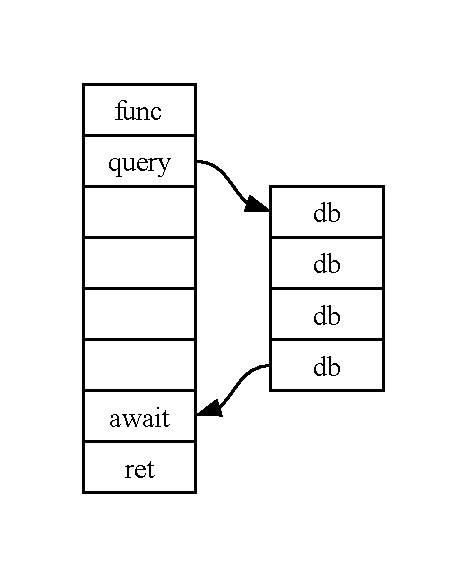
\includegraphics[width=\linewidth]{node_modules/@faaas/double-billing-problem/assets/double-billed-db.pdf}
    \caption{Double billing in action with call to persistent storage. Note that the function handler is idle whilst the DB is executing its query, yet still billed for the entire duration of the function.}
    \label{fig:double-billing-db}
\end{figure}

This is particularly problematic for serverless functions, which are designed to be stateless, and typically communicate with persistent storage to mainain state. This is further compounded by each function instance handling a single request at time.

In other less fine-grained systems such as CaaS, where a single instance handles multiple requests, this is not an issue, as the function can perform other useful work, such as accepting additional requests, while waiting for a response from an asynchronous service.

This issue also manifests more importantly when function invocations are nested as in Figure \ref{fig:double-billing-nested}. Considered an antipattern for this reason\cite{LambdaFunctionsCalling}, nested function invocations lead to a cascading effect of double billing, where each function invocation waits for the next to complete, and is billed for the entire duration of the called function.

\begin{figure}[t]
    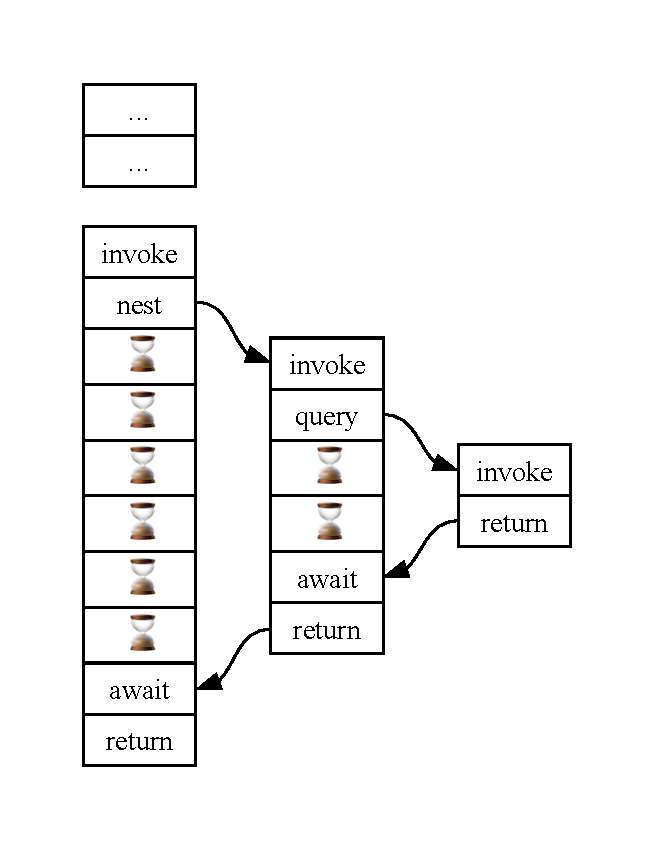
\includegraphics[width=\linewidth]{node_modules/@faaas/double-billing-problem/assets/double-billed-nested.pdf}
    \caption{Double billing in action with nested function invocations. Note that the function handler is idle whilst awaiting the nested invocation, yet still billed for the entire duration of the function.}
    \label{fig:double-billing-nested}
\end{figure}

\todo[inline]{Define CaaS}

\begin{figure*}[t]
    \begin{center}
        %% Creator: Matplotlib, PGF backend
%%
%% To include the figure in your LaTeX document, write
%%   \input{<filename>.pgf}
%%
%% Make sure the required packages are loaded in your preamble
%%   \usepackage{pgf}
%%
%% Also ensure that all the required font packages are loaded; for instance,
%% the lmodern package is sometimes necessary when using math font.
%%   \usepackage{lmodern}
%%
%% Figures using additional raster images can only be included by \input if
%% they are in the same directory as the main LaTeX file. For loading figures
%% from other directories you can use the `import` package
%%   \usepackage{import}
%%
%% and then include the figures with
%%   \import{<path to file>}{<filename>.pgf}
%%
%% Matplotlib used the following preamble
%%   \def\mathdefault#1{#1}
%%   \everymath=\expandafter{\the\everymath\displaystyle}
%%   
%%   \makeatletter\@ifpackageloaded{underscore}{}{\usepackage[strings]{underscore}}\makeatother
%%
\begingroup%
\makeatletter%
\begin{pgfpicture}%
\pgfpathrectangle{\pgfpointorigin}{\pgfqpoint{5.493059in}{3.854278in}}%
\pgfusepath{use as bounding box, clip}%
\begin{pgfscope}%
\pgfsetbuttcap%
\pgfsetmiterjoin%
\definecolor{currentfill}{rgb}{1.000000,1.000000,1.000000}%
\pgfsetfillcolor{currentfill}%
\pgfsetlinewidth{0.000000pt}%
\definecolor{currentstroke}{rgb}{1.000000,1.000000,1.000000}%
\pgfsetstrokecolor{currentstroke}%
\pgfsetdash{}{0pt}%
\pgfpathmoveto{\pgfqpoint{0.000000in}{0.000000in}}%
\pgfpathlineto{\pgfqpoint{5.493059in}{0.000000in}}%
\pgfpathlineto{\pgfqpoint{5.493059in}{3.854278in}}%
\pgfpathlineto{\pgfqpoint{0.000000in}{3.854278in}}%
\pgfpathlineto{\pgfqpoint{0.000000in}{0.000000in}}%
\pgfpathclose%
\pgfusepath{fill}%
\end{pgfscope}%
\begin{pgfscope}%
\pgfsetbuttcap%
\pgfsetmiterjoin%
\definecolor{currentfill}{rgb}{0.917647,0.917647,0.949020}%
\pgfsetfillcolor{currentfill}%
\pgfsetlinewidth{0.000000pt}%
\definecolor{currentstroke}{rgb}{0.000000,0.000000,0.000000}%
\pgfsetstrokecolor{currentstroke}%
\pgfsetstrokeopacity{0.000000}%
\pgfsetdash{}{0pt}%
\pgfpathmoveto{\pgfqpoint{0.800579in}{0.589352in}}%
\pgfpathlineto{\pgfqpoint{5.393059in}{0.589352in}}%
\pgfpathlineto{\pgfqpoint{5.393059in}{3.555205in}}%
\pgfpathlineto{\pgfqpoint{0.800579in}{3.555205in}}%
\pgfpathlineto{\pgfqpoint{0.800579in}{0.589352in}}%
\pgfpathclose%
\pgfusepath{fill}%
\end{pgfscope}%
\begin{pgfscope}%
\pgfpathrectangle{\pgfqpoint{0.800579in}{0.589352in}}{\pgfqpoint{4.592480in}{2.965853in}}%
\pgfusepath{clip}%
\pgfsetroundcap%
\pgfsetroundjoin%
\pgfsetlinewidth{1.003750pt}%
\definecolor{currentstroke}{rgb}{1.000000,1.000000,1.000000}%
\pgfsetstrokecolor{currentstroke}%
\pgfsetdash{}{0pt}%
\pgfpathmoveto{\pgfqpoint{1.009328in}{0.589352in}}%
\pgfpathlineto{\pgfqpoint{1.009328in}{3.555205in}}%
\pgfusepath{stroke}%
\end{pgfscope}%
\begin{pgfscope}%
\definecolor{textcolor}{rgb}{0.150000,0.150000,0.150000}%
\pgfsetstrokecolor{textcolor}%
\pgfsetfillcolor{textcolor}%
\pgftext[x=1.009328in,y=0.457407in,,top]{\color{textcolor}{\rmfamily\fontsize{11.000000}{13.200000}\selectfont\catcode`\^=\active\def^{\ifmmode\sp\else\^{}\fi}\catcode`\%=\active\def%{\%}$\mathdefault{2^{7}}$}}%
\end{pgfscope}%
\begin{pgfscope}%
\pgfpathrectangle{\pgfqpoint{0.800579in}{0.589352in}}{\pgfqpoint{4.592480in}{2.965853in}}%
\pgfusepath{clip}%
\pgfsetroundcap%
\pgfsetroundjoin%
\pgfsetlinewidth{1.003750pt}%
\definecolor{currentstroke}{rgb}{1.000000,1.000000,1.000000}%
\pgfsetstrokecolor{currentstroke}%
\pgfsetdash{}{0pt}%
\pgfpathmoveto{\pgfqpoint{2.053074in}{0.589352in}}%
\pgfpathlineto{\pgfqpoint{2.053074in}{3.555205in}}%
\pgfusepath{stroke}%
\end{pgfscope}%
\begin{pgfscope}%
\definecolor{textcolor}{rgb}{0.150000,0.150000,0.150000}%
\pgfsetstrokecolor{textcolor}%
\pgfsetfillcolor{textcolor}%
\pgftext[x=2.053074in,y=0.457407in,,top]{\color{textcolor}{\rmfamily\fontsize{11.000000}{13.200000}\selectfont\catcode`\^=\active\def^{\ifmmode\sp\else\^{}\fi}\catcode`\%=\active\def%{\%}$\mathdefault{2^{8}}$}}%
\end{pgfscope}%
\begin{pgfscope}%
\pgfpathrectangle{\pgfqpoint{0.800579in}{0.589352in}}{\pgfqpoint{4.592480in}{2.965853in}}%
\pgfusepath{clip}%
\pgfsetroundcap%
\pgfsetroundjoin%
\pgfsetlinewidth{1.003750pt}%
\definecolor{currentstroke}{rgb}{1.000000,1.000000,1.000000}%
\pgfsetstrokecolor{currentstroke}%
\pgfsetdash{}{0pt}%
\pgfpathmoveto{\pgfqpoint{3.096819in}{0.589352in}}%
\pgfpathlineto{\pgfqpoint{3.096819in}{3.555205in}}%
\pgfusepath{stroke}%
\end{pgfscope}%
\begin{pgfscope}%
\definecolor{textcolor}{rgb}{0.150000,0.150000,0.150000}%
\pgfsetstrokecolor{textcolor}%
\pgfsetfillcolor{textcolor}%
\pgftext[x=3.096819in,y=0.457407in,,top]{\color{textcolor}{\rmfamily\fontsize{11.000000}{13.200000}\selectfont\catcode`\^=\active\def^{\ifmmode\sp\else\^{}\fi}\catcode`\%=\active\def%{\%}$\mathdefault{2^{9}}$}}%
\end{pgfscope}%
\begin{pgfscope}%
\pgfpathrectangle{\pgfqpoint{0.800579in}{0.589352in}}{\pgfqpoint{4.592480in}{2.965853in}}%
\pgfusepath{clip}%
\pgfsetroundcap%
\pgfsetroundjoin%
\pgfsetlinewidth{1.003750pt}%
\definecolor{currentstroke}{rgb}{1.000000,1.000000,1.000000}%
\pgfsetstrokecolor{currentstroke}%
\pgfsetdash{}{0pt}%
\pgfpathmoveto{\pgfqpoint{4.140564in}{0.589352in}}%
\pgfpathlineto{\pgfqpoint{4.140564in}{3.555205in}}%
\pgfusepath{stroke}%
\end{pgfscope}%
\begin{pgfscope}%
\definecolor{textcolor}{rgb}{0.150000,0.150000,0.150000}%
\pgfsetstrokecolor{textcolor}%
\pgfsetfillcolor{textcolor}%
\pgftext[x=4.140564in,y=0.457407in,,top]{\color{textcolor}{\rmfamily\fontsize{11.000000}{13.200000}\selectfont\catcode`\^=\active\def^{\ifmmode\sp\else\^{}\fi}\catcode`\%=\active\def%{\%}$\mathdefault{2^{10}}$}}%
\end{pgfscope}%
\begin{pgfscope}%
\pgfpathrectangle{\pgfqpoint{0.800579in}{0.589352in}}{\pgfqpoint{4.592480in}{2.965853in}}%
\pgfusepath{clip}%
\pgfsetroundcap%
\pgfsetroundjoin%
\pgfsetlinewidth{1.003750pt}%
\definecolor{currentstroke}{rgb}{1.000000,1.000000,1.000000}%
\pgfsetstrokecolor{currentstroke}%
\pgfsetdash{}{0pt}%
\pgfpathmoveto{\pgfqpoint{5.184310in}{0.589352in}}%
\pgfpathlineto{\pgfqpoint{5.184310in}{3.555205in}}%
\pgfusepath{stroke}%
\end{pgfscope}%
\begin{pgfscope}%
\definecolor{textcolor}{rgb}{0.150000,0.150000,0.150000}%
\pgfsetstrokecolor{textcolor}%
\pgfsetfillcolor{textcolor}%
\pgftext[x=5.184310in,y=0.457407in,,top]{\color{textcolor}{\rmfamily\fontsize{11.000000}{13.200000}\selectfont\catcode`\^=\active\def^{\ifmmode\sp\else\^{}\fi}\catcode`\%=\active\def%{\%}$\mathdefault{2^{11}}$}}%
\end{pgfscope}%
\begin{pgfscope}%
\definecolor{textcolor}{rgb}{0.150000,0.150000,0.150000}%
\pgfsetstrokecolor{textcolor}%
\pgfsetfillcolor{textcolor}%
\pgftext[x=3.096819in,y=0.266667in,,top]{\color{textcolor}{\rmfamily\fontsize{12.000000}{14.400000}\selectfont\catcode`\^=\active\def^{\ifmmode\sp\else\^{}\fi}\catcode`\%=\active\def%{\%}Memory (MB)}}%
\end{pgfscope}%
\begin{pgfscope}%
\pgfpathrectangle{\pgfqpoint{0.800579in}{0.589352in}}{\pgfqpoint{4.592480in}{2.965853in}}%
\pgfusepath{clip}%
\pgfsetroundcap%
\pgfsetroundjoin%
\pgfsetlinewidth{1.003750pt}%
\definecolor{currentstroke}{rgb}{1.000000,1.000000,1.000000}%
\pgfsetstrokecolor{currentstroke}%
\pgfsetdash{}{0pt}%
\pgfpathmoveto{\pgfqpoint{0.800579in}{0.627869in}}%
\pgfpathlineto{\pgfqpoint{5.393059in}{0.627869in}}%
\pgfusepath{stroke}%
\end{pgfscope}%
\begin{pgfscope}%
\definecolor{textcolor}{rgb}{0.150000,0.150000,0.150000}%
\pgfsetstrokecolor{textcolor}%
\pgfsetfillcolor{textcolor}%
\pgftext[x=0.322222in, y=0.575063in, left, base]{\color{textcolor}{\rmfamily\fontsize{11.000000}{13.200000}\selectfont\catcode`\^=\active\def^{\ifmmode\sp\else\^{}\fi}\catcode`\%=\active\def%{\%}$\mathdefault{0.000}$}}%
\end{pgfscope}%
\begin{pgfscope}%
\pgfpathrectangle{\pgfqpoint{0.800579in}{0.589352in}}{\pgfqpoint{4.592480in}{2.965853in}}%
\pgfusepath{clip}%
\pgfsetroundcap%
\pgfsetroundjoin%
\pgfsetlinewidth{1.003750pt}%
\definecolor{currentstroke}{rgb}{1.000000,1.000000,1.000000}%
\pgfsetstrokecolor{currentstroke}%
\pgfsetdash{}{0pt}%
\pgfpathmoveto{\pgfqpoint{0.800579in}{1.029094in}}%
\pgfpathlineto{\pgfqpoint{5.393059in}{1.029094in}}%
\pgfusepath{stroke}%
\end{pgfscope}%
\begin{pgfscope}%
\definecolor{textcolor}{rgb}{0.150000,0.150000,0.150000}%
\pgfsetstrokecolor{textcolor}%
\pgfsetfillcolor{textcolor}%
\pgftext[x=0.322222in, y=0.976287in, left, base]{\color{textcolor}{\rmfamily\fontsize{11.000000}{13.200000}\selectfont\catcode`\^=\active\def^{\ifmmode\sp\else\^{}\fi}\catcode`\%=\active\def%{\%}$\mathdefault{0.025}$}}%
\end{pgfscope}%
\begin{pgfscope}%
\pgfpathrectangle{\pgfqpoint{0.800579in}{0.589352in}}{\pgfqpoint{4.592480in}{2.965853in}}%
\pgfusepath{clip}%
\pgfsetroundcap%
\pgfsetroundjoin%
\pgfsetlinewidth{1.003750pt}%
\definecolor{currentstroke}{rgb}{1.000000,1.000000,1.000000}%
\pgfsetstrokecolor{currentstroke}%
\pgfsetdash{}{0pt}%
\pgfpathmoveto{\pgfqpoint{0.800579in}{1.430319in}}%
\pgfpathlineto{\pgfqpoint{5.393059in}{1.430319in}}%
\pgfusepath{stroke}%
\end{pgfscope}%
\begin{pgfscope}%
\definecolor{textcolor}{rgb}{0.150000,0.150000,0.150000}%
\pgfsetstrokecolor{textcolor}%
\pgfsetfillcolor{textcolor}%
\pgftext[x=0.322222in, y=1.377512in, left, base]{\color{textcolor}{\rmfamily\fontsize{11.000000}{13.200000}\selectfont\catcode`\^=\active\def^{\ifmmode\sp\else\^{}\fi}\catcode`\%=\active\def%{\%}$\mathdefault{0.050}$}}%
\end{pgfscope}%
\begin{pgfscope}%
\pgfpathrectangle{\pgfqpoint{0.800579in}{0.589352in}}{\pgfqpoint{4.592480in}{2.965853in}}%
\pgfusepath{clip}%
\pgfsetroundcap%
\pgfsetroundjoin%
\pgfsetlinewidth{1.003750pt}%
\definecolor{currentstroke}{rgb}{1.000000,1.000000,1.000000}%
\pgfsetstrokecolor{currentstroke}%
\pgfsetdash{}{0pt}%
\pgfpathmoveto{\pgfqpoint{0.800579in}{1.831543in}}%
\pgfpathlineto{\pgfqpoint{5.393059in}{1.831543in}}%
\pgfusepath{stroke}%
\end{pgfscope}%
\begin{pgfscope}%
\definecolor{textcolor}{rgb}{0.150000,0.150000,0.150000}%
\pgfsetstrokecolor{textcolor}%
\pgfsetfillcolor{textcolor}%
\pgftext[x=0.322222in, y=1.778737in, left, base]{\color{textcolor}{\rmfamily\fontsize{11.000000}{13.200000}\selectfont\catcode`\^=\active\def^{\ifmmode\sp\else\^{}\fi}\catcode`\%=\active\def%{\%}$\mathdefault{0.075}$}}%
\end{pgfscope}%
\begin{pgfscope}%
\pgfpathrectangle{\pgfqpoint{0.800579in}{0.589352in}}{\pgfqpoint{4.592480in}{2.965853in}}%
\pgfusepath{clip}%
\pgfsetroundcap%
\pgfsetroundjoin%
\pgfsetlinewidth{1.003750pt}%
\definecolor{currentstroke}{rgb}{1.000000,1.000000,1.000000}%
\pgfsetstrokecolor{currentstroke}%
\pgfsetdash{}{0pt}%
\pgfpathmoveto{\pgfqpoint{0.800579in}{2.232768in}}%
\pgfpathlineto{\pgfqpoint{5.393059in}{2.232768in}}%
\pgfusepath{stroke}%
\end{pgfscope}%
\begin{pgfscope}%
\definecolor{textcolor}{rgb}{0.150000,0.150000,0.150000}%
\pgfsetstrokecolor{textcolor}%
\pgfsetfillcolor{textcolor}%
\pgftext[x=0.322222in, y=2.179961in, left, base]{\color{textcolor}{\rmfamily\fontsize{11.000000}{13.200000}\selectfont\catcode`\^=\active\def^{\ifmmode\sp\else\^{}\fi}\catcode`\%=\active\def%{\%}$\mathdefault{0.100}$}}%
\end{pgfscope}%
\begin{pgfscope}%
\pgfpathrectangle{\pgfqpoint{0.800579in}{0.589352in}}{\pgfqpoint{4.592480in}{2.965853in}}%
\pgfusepath{clip}%
\pgfsetroundcap%
\pgfsetroundjoin%
\pgfsetlinewidth{1.003750pt}%
\definecolor{currentstroke}{rgb}{1.000000,1.000000,1.000000}%
\pgfsetstrokecolor{currentstroke}%
\pgfsetdash{}{0pt}%
\pgfpathmoveto{\pgfqpoint{0.800579in}{2.633993in}}%
\pgfpathlineto{\pgfqpoint{5.393059in}{2.633993in}}%
\pgfusepath{stroke}%
\end{pgfscope}%
\begin{pgfscope}%
\definecolor{textcolor}{rgb}{0.150000,0.150000,0.150000}%
\pgfsetstrokecolor{textcolor}%
\pgfsetfillcolor{textcolor}%
\pgftext[x=0.322222in, y=2.581186in, left, base]{\color{textcolor}{\rmfamily\fontsize{11.000000}{13.200000}\selectfont\catcode`\^=\active\def^{\ifmmode\sp\else\^{}\fi}\catcode`\%=\active\def%{\%}$\mathdefault{0.125}$}}%
\end{pgfscope}%
\begin{pgfscope}%
\pgfpathrectangle{\pgfqpoint{0.800579in}{0.589352in}}{\pgfqpoint{4.592480in}{2.965853in}}%
\pgfusepath{clip}%
\pgfsetroundcap%
\pgfsetroundjoin%
\pgfsetlinewidth{1.003750pt}%
\definecolor{currentstroke}{rgb}{1.000000,1.000000,1.000000}%
\pgfsetstrokecolor{currentstroke}%
\pgfsetdash{}{0pt}%
\pgfpathmoveto{\pgfqpoint{0.800579in}{3.035218in}}%
\pgfpathlineto{\pgfqpoint{5.393059in}{3.035218in}}%
\pgfusepath{stroke}%
\end{pgfscope}%
\begin{pgfscope}%
\definecolor{textcolor}{rgb}{0.150000,0.150000,0.150000}%
\pgfsetstrokecolor{textcolor}%
\pgfsetfillcolor{textcolor}%
\pgftext[x=0.322222in, y=2.982411in, left, base]{\color{textcolor}{\rmfamily\fontsize{11.000000}{13.200000}\selectfont\catcode`\^=\active\def^{\ifmmode\sp\else\^{}\fi}\catcode`\%=\active\def%{\%}$\mathdefault{0.150}$}}%
\end{pgfscope}%
\begin{pgfscope}%
\pgfpathrectangle{\pgfqpoint{0.800579in}{0.589352in}}{\pgfqpoint{4.592480in}{2.965853in}}%
\pgfusepath{clip}%
\pgfsetroundcap%
\pgfsetroundjoin%
\pgfsetlinewidth{1.003750pt}%
\definecolor{currentstroke}{rgb}{1.000000,1.000000,1.000000}%
\pgfsetstrokecolor{currentstroke}%
\pgfsetdash{}{0pt}%
\pgfpathmoveto{\pgfqpoint{0.800579in}{3.436442in}}%
\pgfpathlineto{\pgfqpoint{5.393059in}{3.436442in}}%
\pgfusepath{stroke}%
\end{pgfscope}%
\begin{pgfscope}%
\definecolor{textcolor}{rgb}{0.150000,0.150000,0.150000}%
\pgfsetstrokecolor{textcolor}%
\pgfsetfillcolor{textcolor}%
\pgftext[x=0.322222in, y=3.383636in, left, base]{\color{textcolor}{\rmfamily\fontsize{11.000000}{13.200000}\selectfont\catcode`\^=\active\def^{\ifmmode\sp\else\^{}\fi}\catcode`\%=\active\def%{\%}$\mathdefault{0.175}$}}%
\end{pgfscope}%
\begin{pgfscope}%
\definecolor{textcolor}{rgb}{0.150000,0.150000,0.150000}%
\pgfsetstrokecolor{textcolor}%
\pgfsetfillcolor{textcolor}%
\pgftext[x=0.266667in,y=2.072278in,,bottom,rotate=90.000000]{\color{textcolor}{\rmfamily\fontsize{12.000000}{14.400000}\selectfont\catcode`\^=\active\def^{\ifmmode\sp\else\^{}\fi}\catcode`\%=\active\def%{\%}Yield time (s)}}%
\end{pgfscope}%
\begin{pgfscope}%
\pgfpathrectangle{\pgfqpoint{0.800579in}{0.589352in}}{\pgfqpoint{4.592480in}{2.965853in}}%
\pgfusepath{clip}%
\pgfsetbuttcap%
\pgfsetmiterjoin%
\definecolor{currentfill}{rgb}{0.768627,0.305882,0.321569}%
\pgfsetfillcolor{currentfill}%
\pgfsetfillopacity{0.200000}%
\pgfsetlinewidth{1.003750pt}%
\definecolor{currentstroke}{rgb}{0.768627,0.305882,0.321569}%
\pgfsetstrokecolor{currentstroke}%
\pgfsetstrokeopacity{0.200000}%
\pgfsetdash{}{0pt}%
\pgfpathmoveto{\pgfqpoint{0.800579in}{1.590809in}}%
\pgfpathlineto{\pgfqpoint{0.800579in}{2.072278in}}%
\pgfpathlineto{\pgfqpoint{5.393059in}{2.072278in}}%
\pgfpathlineto{\pgfqpoint{5.393059in}{1.590809in}}%
\pgfpathlineto{\pgfqpoint{0.800579in}{1.590809in}}%
\pgfpathclose%
\pgfusepath{stroke,fill}%
\end{pgfscope}%
\begin{pgfscope}%
\pgfpathrectangle{\pgfqpoint{0.800579in}{0.589352in}}{\pgfqpoint{4.592480in}{2.965853in}}%
\pgfusepath{clip}%
\pgfsetbuttcap%
\pgfsetmiterjoin%
\definecolor{currentfill}{rgb}{0.298039,0.447059,0.690196}%
\pgfsetfillcolor{currentfill}%
\pgfsetfillopacity{0.200000}%
\pgfsetlinewidth{1.003750pt}%
\definecolor{currentstroke}{rgb}{0.298039,0.447059,0.690196}%
\pgfsetstrokecolor{currentstroke}%
\pgfsetstrokeopacity{0.200000}%
\pgfsetdash{}{0pt}%
\pgfpathmoveto{\pgfqpoint{0.800579in}{0.788359in}}%
\pgfpathlineto{\pgfqpoint{0.800579in}{1.029094in}}%
\pgfpathlineto{\pgfqpoint{5.393059in}{1.029094in}}%
\pgfpathlineto{\pgfqpoint{5.393059in}{0.788359in}}%
\pgfpathlineto{\pgfqpoint{0.800579in}{0.788359in}}%
\pgfpathclose%
\pgfusepath{stroke,fill}%
\end{pgfscope}%
\begin{pgfscope}%
\pgfpathrectangle{\pgfqpoint{0.800579in}{0.589352in}}{\pgfqpoint{4.592480in}{2.965853in}}%
\pgfusepath{clip}%
\pgfsetroundcap%
\pgfsetroundjoin%
\pgfsetlinewidth{1.505625pt}%
\definecolor{currentstroke}{rgb}{0.298039,0.447059,0.690196}%
\pgfsetstrokecolor{currentstroke}%
\pgfsetdash{}{0pt}%
\pgfpathmoveto{\pgfqpoint{1.009328in}{2.168572in}}%
\pgfpathlineto{\pgfqpoint{1.021047in}{2.168572in}}%
\pgfpathlineto{\pgfqpoint{1.044213in}{2.136474in}}%
\pgfpathlineto{\pgfqpoint{1.055664in}{2.136474in}}%
\pgfpathlineto{\pgfqpoint{1.078309in}{2.104376in}}%
\pgfpathlineto{\pgfqpoint{1.089504in}{2.104376in}}%
\pgfpathlineto{\pgfqpoint{1.111649in}{2.072278in}}%
\pgfpathlineto{\pgfqpoint{1.122600in}{2.072278in}}%
\pgfpathlineto{\pgfqpoint{1.144267in}{2.040180in}}%
\pgfpathlineto{\pgfqpoint{1.154984in}{2.040180in}}%
\pgfpathlineto{\pgfqpoint{1.176193in}{2.008082in}}%
\pgfpathlineto{\pgfqpoint{1.186687in}{2.008082in}}%
\pgfpathlineto{\pgfqpoint{1.197108in}{1.992033in}}%
\pgfpathlineto{\pgfqpoint{1.207457in}{1.992033in}}%
\pgfpathlineto{\pgfqpoint{1.217735in}{1.975984in}}%
\pgfpathlineto{\pgfqpoint{1.227944in}{1.975984in}}%
\pgfpathlineto{\pgfqpoint{1.248157in}{1.943886in}}%
\pgfpathlineto{\pgfqpoint{1.258162in}{1.943886in}}%
\pgfpathlineto{\pgfqpoint{1.268101in}{1.927837in}}%
\pgfpathlineto{\pgfqpoint{1.277976in}{1.927837in}}%
\pgfpathlineto{\pgfqpoint{1.287785in}{1.911788in}}%
\pgfpathlineto{\pgfqpoint{1.297532in}{1.911788in}}%
\pgfpathlineto{\pgfqpoint{1.307215in}{1.895739in}}%
\pgfpathlineto{\pgfqpoint{1.316837in}{1.895739in}}%
\pgfpathlineto{\pgfqpoint{1.326398in}{1.879690in}}%
\pgfpathlineto{\pgfqpoint{1.335898in}{1.879690in}}%
\pgfpathlineto{\pgfqpoint{1.345339in}{1.863641in}}%
\pgfpathlineto{\pgfqpoint{1.354721in}{1.863641in}}%
\pgfpathlineto{\pgfqpoint{1.364045in}{1.847592in}}%
\pgfpathlineto{\pgfqpoint{1.373312in}{1.847592in}}%
\pgfpathlineto{\pgfqpoint{1.382521in}{1.831543in}}%
\pgfpathlineto{\pgfqpoint{1.400774in}{1.831543in}}%
\pgfpathlineto{\pgfqpoint{1.409818in}{1.815494in}}%
\pgfpathlineto{\pgfqpoint{1.418808in}{1.815494in}}%
\pgfpathlineto{\pgfqpoint{1.427744in}{1.799445in}}%
\pgfpathlineto{\pgfqpoint{1.436628in}{1.799445in}}%
\pgfpathlineto{\pgfqpoint{1.445460in}{1.783396in}}%
\pgfpathlineto{\pgfqpoint{1.462969in}{1.783396in}}%
\pgfpathlineto{\pgfqpoint{1.471648in}{1.767347in}}%
\pgfpathlineto{\pgfqpoint{1.480278in}{1.767347in}}%
\pgfpathlineto{\pgfqpoint{1.488858in}{1.751299in}}%
\pgfpathlineto{\pgfqpoint{1.505873in}{1.751299in}}%
\pgfpathlineto{\pgfqpoint{1.514309in}{1.735250in}}%
\pgfpathlineto{\pgfqpoint{1.522698in}{1.735250in}}%
\pgfpathlineto{\pgfqpoint{1.531040in}{1.719201in}}%
\pgfpathlineto{\pgfqpoint{1.547588in}{1.719201in}}%
\pgfpathlineto{\pgfqpoint{1.555794in}{1.703152in}}%
\pgfpathlineto{\pgfqpoint{1.572073in}{1.703152in}}%
\pgfpathlineto{\pgfqpoint{1.580147in}{1.687103in}}%
\pgfpathlineto{\pgfqpoint{1.596166in}{1.687103in}}%
\pgfpathlineto{\pgfqpoint{1.604112in}{1.671054in}}%
\pgfpathlineto{\pgfqpoint{1.612017in}{1.671054in}}%
\pgfpathlineto{\pgfqpoint{1.619880in}{1.655005in}}%
\pgfpathlineto{\pgfqpoint{1.643226in}{1.655005in}}%
\pgfpathlineto{\pgfqpoint{1.650929in}{1.638956in}}%
\pgfpathlineto{\pgfqpoint{1.666216in}{1.638956in}}%
\pgfpathlineto{\pgfqpoint{1.673802in}{1.622907in}}%
\pgfpathlineto{\pgfqpoint{1.688860in}{1.622907in}}%
\pgfpathlineto{\pgfqpoint{1.696333in}{1.606858in}}%
\pgfpathlineto{\pgfqpoint{1.711169in}{1.606858in}}%
\pgfpathlineto{\pgfqpoint{1.718532in}{1.590809in}}%
\pgfpathlineto{\pgfqpoint{1.740409in}{1.590809in}}%
\pgfpathlineto{\pgfqpoint{1.747631in}{1.574760in}}%
\pgfpathlineto{\pgfqpoint{1.761972in}{1.574760in}}%
\pgfpathlineto{\pgfqpoint{1.769092in}{1.558711in}}%
\pgfpathlineto{\pgfqpoint{1.790251in}{1.558711in}}%
\pgfpathlineto{\pgfqpoint{1.797239in}{1.542662in}}%
\pgfpathlineto{\pgfqpoint{1.818009in}{1.542662in}}%
\pgfpathlineto{\pgfqpoint{1.824869in}{1.526613in}}%
\pgfpathlineto{\pgfqpoint{1.845264in}{1.526613in}}%
\pgfpathlineto{\pgfqpoint{1.852001in}{1.510564in}}%
\pgfpathlineto{\pgfqpoint{1.872034in}{1.510564in}}%
\pgfpathlineto{\pgfqpoint{1.878653in}{1.494515in}}%
\pgfpathlineto{\pgfqpoint{1.898337in}{1.494515in}}%
\pgfpathlineto{\pgfqpoint{1.904842in}{1.478466in}}%
\pgfpathlineto{\pgfqpoint{1.930583in}{1.478466in}}%
\pgfpathlineto{\pgfqpoint{1.936950in}{1.462417in}}%
\pgfpathlineto{\pgfqpoint{1.955891in}{1.462417in}}%
\pgfpathlineto{\pgfqpoint{1.962152in}{1.446368in}}%
\pgfpathlineto{\pgfqpoint{1.986940in}{1.446368in}}%
\pgfpathlineto{\pgfqpoint{1.993073in}{1.430319in}}%
\pgfpathlineto{\pgfqpoint{2.017361in}{1.430319in}}%
\pgfpathlineto{\pgfqpoint{2.023372in}{1.414270in}}%
\pgfpathlineto{\pgfqpoint{2.047180in}{1.414270in}}%
\pgfpathlineto{\pgfqpoint{2.053074in}{1.398221in}}%
\pgfpathlineto{\pgfqpoint{2.082200in}{1.398221in}}%
\pgfpathlineto{\pgfqpoint{2.087959in}{1.382172in}}%
\pgfpathlineto{\pgfqpoint{2.116425in}{1.382172in}}%
\pgfpathlineto{\pgfqpoint{2.122054in}{1.366123in}}%
\pgfpathlineto{\pgfqpoint{2.149888in}{1.366123in}}%
\pgfpathlineto{\pgfqpoint{2.155394in}{1.350074in}}%
\pgfpathlineto{\pgfqpoint{2.182625in}{1.350074in}}%
\pgfpathlineto{\pgfqpoint{2.188012in}{1.334025in}}%
\pgfpathlineto{\pgfqpoint{2.214664in}{1.334025in}}%
\pgfpathlineto{\pgfqpoint{2.219939in}{1.317976in}}%
\pgfpathlineto{\pgfqpoint{2.251202in}{1.317976in}}%
\pgfpathlineto{\pgfqpoint{2.256350in}{1.301927in}}%
\pgfpathlineto{\pgfqpoint{2.286874in}{1.301927in}}%
\pgfpathlineto{\pgfqpoint{2.291902in}{1.285878in}}%
\pgfpathlineto{\pgfqpoint{2.326634in}{1.285878in}}%
\pgfpathlineto{\pgfqpoint{2.331531in}{1.269829in}}%
\pgfpathlineto{\pgfqpoint{2.365371in}{1.269829in}}%
\pgfpathlineto{\pgfqpoint{2.370143in}{1.253780in}}%
\pgfpathlineto{\pgfqpoint{2.403136in}{1.253780in}}%
\pgfpathlineto{\pgfqpoint{2.407790in}{1.237731in}}%
\pgfpathlineto{\pgfqpoint{2.444519in}{1.237731in}}%
\pgfpathlineto{\pgfqpoint{2.449048in}{1.221682in}}%
\pgfpathlineto{\pgfqpoint{2.484796in}{1.221682in}}%
\pgfpathlineto{\pgfqpoint{2.489205in}{1.205633in}}%
\pgfpathlineto{\pgfqpoint{2.528319in}{1.205633in}}%
\pgfpathlineto{\pgfqpoint{2.532603in}{1.189584in}}%
\pgfpathlineto{\pgfqpoint{2.570620in}{1.189584in}}%
\pgfpathlineto{\pgfqpoint{2.574785in}{1.173535in}}%
\pgfpathlineto{\pgfqpoint{2.615818in}{1.173535in}}%
\pgfpathlineto{\pgfqpoint{2.619861in}{1.157486in}}%
\pgfpathlineto{\pgfqpoint{2.659699in}{1.157486in}}%
\pgfpathlineto{\pgfqpoint{2.663625in}{1.141437in}}%
\pgfpathlineto{\pgfqpoint{2.709962in}{1.141437in}}%
\pgfpathlineto{\pgfqpoint{2.713759in}{1.125388in}}%
\pgfpathlineto{\pgfqpoint{2.758601in}{1.125388in}}%
\pgfpathlineto{\pgfqpoint{2.762278in}{1.109339in}}%
\pgfpathlineto{\pgfqpoint{2.809282in}{1.109339in}}%
\pgfpathlineto{\pgfqpoint{2.812837in}{1.093290in}}%
\pgfpathlineto{\pgfqpoint{2.861754in}{1.093290in}}%
\pgfpathlineto{\pgfqpoint{2.865188in}{1.077241in}}%
\pgfpathlineto{\pgfqpoint{2.919093in}{1.077241in}}%
\pgfpathlineto{\pgfqpoint{2.922399in}{1.061192in}}%
\pgfpathlineto{\pgfqpoint{2.974328in}{1.061192in}}%
\pgfpathlineto{\pgfqpoint{2.977515in}{1.045143in}}%
\pgfpathlineto{\pgfqpoint{3.033755in}{1.045143in}}%
\pgfpathlineto{\pgfqpoint{3.036819in}{1.029094in}}%
\pgfpathlineto{\pgfqpoint{3.093875in}{1.029094in}}%
\pgfpathlineto{\pgfqpoint{3.096819in}{1.013045in}}%
\pgfpathlineto{\pgfqpoint{3.160170in}{1.013045in}}%
\pgfpathlineto{\pgfqpoint{3.162987in}{0.996996in}}%
\pgfpathlineto{\pgfqpoint{3.226370in}{0.996996in}}%
\pgfpathlineto{\pgfqpoint{3.229066in}{0.980947in}}%
\pgfpathlineto{\pgfqpoint{3.297524in}{0.980947in}}%
\pgfpathlineto{\pgfqpoint{3.300095in}{0.964898in}}%
\pgfpathlineto{\pgfqpoint{3.370379in}{0.964898in}}%
\pgfpathlineto{\pgfqpoint{3.372830in}{0.948849in}}%
\pgfpathlineto{\pgfqpoint{3.446881in}{0.948849in}}%
\pgfpathlineto{\pgfqpoint{3.449210in}{0.932800in}}%
\pgfpathlineto{\pgfqpoint{3.528541in}{0.932800in}}%
\pgfpathlineto{\pgfqpoint{3.530747in}{0.916751in}}%
\pgfpathlineto{\pgfqpoint{3.614365in}{0.916751in}}%
\pgfpathlineto{\pgfqpoint{3.616449in}{0.900702in}}%
\pgfpathlineto{\pgfqpoint{3.705409in}{0.900702in}}%
\pgfpathlineto{\pgfqpoint{3.707371in}{0.884653in}}%
\pgfpathlineto{\pgfqpoint{3.804186in}{0.884653in}}%
\pgfpathlineto{\pgfqpoint{3.806023in}{0.868604in}}%
\pgfpathlineto{\pgfqpoint{3.907217in}{0.868604in}}%
\pgfpathlineto{\pgfqpoint{3.908933in}{0.852555in}}%
\pgfpathlineto{\pgfqpoint{4.019668in}{0.852555in}}%
\pgfpathlineto{\pgfqpoint{4.021260in}{0.836506in}}%
\pgfpathlineto{\pgfqpoint{4.139093in}{0.836506in}}%
\pgfpathlineto{\pgfqpoint{4.140564in}{0.820457in}}%
\pgfpathlineto{\pgfqpoint{4.271464in}{0.820457in}}%
\pgfpathlineto{\pgfqpoint{4.272811in}{0.804408in}}%
\pgfpathlineto{\pgfqpoint{4.414125in}{0.804408in}}%
\pgfpathlineto{\pgfqpoint{4.415350in}{0.788359in}}%
\pgfpathlineto{\pgfqpoint{4.573390in}{0.788359in}}%
\pgfpathlineto{\pgfqpoint{4.575595in}{0.772310in}}%
\pgfpathlineto{\pgfqpoint{4.750135in}{0.772310in}}%
\pgfpathlineto{\pgfqpoint{4.752096in}{0.756261in}}%
\pgfpathlineto{\pgfqpoint{4.951821in}{0.756261in}}%
\pgfpathlineto{\pgfqpoint{4.953536in}{0.740212in}}%
\pgfpathlineto{\pgfqpoint{5.183574in}{0.740212in}}%
\pgfpathlineto{\pgfqpoint{5.184310in}{0.724163in}}%
\pgfpathlineto{\pgfqpoint{5.184310in}{0.724163in}}%
\pgfusepath{stroke}%
\end{pgfscope}%
\begin{pgfscope}%
\pgfpathrectangle{\pgfqpoint{0.800579in}{0.589352in}}{\pgfqpoint{4.592480in}{2.965853in}}%
\pgfusepath{clip}%
\pgfsetroundcap%
\pgfsetroundjoin%
\pgfsetlinewidth{1.505625pt}%
\definecolor{currentstroke}{rgb}{0.866667,0.517647,0.321569}%
\pgfsetstrokecolor{currentstroke}%
\pgfsetdash{}{0pt}%
\pgfpathmoveto{\pgfqpoint{1.009328in}{2.232768in}}%
\pgfpathlineto{\pgfqpoint{2.047180in}{2.232768in}}%
\pgfpathlineto{\pgfqpoint{2.053074in}{1.430319in}}%
\pgfpathlineto{\pgfqpoint{2.659699in}{1.430319in}}%
\pgfpathlineto{\pgfqpoint{2.663625in}{1.173535in}}%
\pgfpathlineto{\pgfqpoint{3.093875in}{1.173535in}}%
\pgfpathlineto{\pgfqpoint{3.096819in}{1.029094in}}%
\pgfpathlineto{\pgfqpoint{3.430475in}{1.029094in}}%
\pgfpathlineto{\pgfqpoint{3.432830in}{0.948849in}}%
\pgfpathlineto{\pgfqpoint{3.705409in}{0.948849in}}%
\pgfpathlineto{\pgfqpoint{3.707371in}{0.900702in}}%
\pgfpathlineto{\pgfqpoint{3.937810in}{0.900702in}}%
\pgfpathlineto{\pgfqpoint{3.939492in}{0.868604in}}%
\pgfpathlineto{\pgfqpoint{4.139093in}{0.868604in}}%
\pgfpathlineto{\pgfqpoint{4.140564in}{0.836506in}}%
\pgfpathlineto{\pgfqpoint{4.316615in}{0.836506in}}%
\pgfpathlineto{\pgfqpoint{4.317923in}{0.820457in}}%
\pgfpathlineto{\pgfqpoint{4.475398in}{0.820457in}}%
\pgfpathlineto{\pgfqpoint{4.476575in}{0.788359in}}%
\pgfpathlineto{\pgfqpoint{4.750135in}{0.788359in}}%
\pgfpathlineto{\pgfqpoint{4.752096in}{0.772310in}}%
\pgfpathlineto{\pgfqpoint{5.184310in}{0.772310in}}%
\pgfpathlineto{\pgfqpoint{5.184310in}{0.772310in}}%
\pgfusepath{stroke}%
\end{pgfscope}%
\begin{pgfscope}%
\pgfpathrectangle{\pgfqpoint{0.800579in}{0.589352in}}{\pgfqpoint{4.592480in}{2.965853in}}%
\pgfusepath{clip}%
\pgfsetroundcap%
\pgfsetroundjoin%
\pgfsetlinewidth{1.505625pt}%
\definecolor{currentstroke}{rgb}{0.333333,0.658824,0.407843}%
\pgfsetstrokecolor{currentstroke}%
\pgfsetdash{}{0pt}%
\pgfpathmoveto{\pgfqpoint{1.009328in}{3.420393in}}%
\pgfpathlineto{\pgfqpoint{2.047180in}{3.420393in}}%
\pgfpathlineto{\pgfqpoint{2.053074in}{2.024131in}}%
\pgfpathlineto{\pgfqpoint{3.093875in}{2.024131in}}%
\pgfpathlineto{\pgfqpoint{3.096819in}{1.334025in}}%
\pgfpathlineto{\pgfqpoint{4.139093in}{1.334025in}}%
\pgfpathlineto{\pgfqpoint{4.140564in}{1.029094in}}%
\pgfpathlineto{\pgfqpoint{5.183574in}{1.029094in}}%
\pgfpathlineto{\pgfqpoint{5.184310in}{0.852555in}}%
\pgfpathlineto{\pgfqpoint{5.184310in}{0.852555in}}%
\pgfusepath{stroke}%
\end{pgfscope}%
\begin{pgfscope}%
\pgfpathrectangle{\pgfqpoint{0.800579in}{0.589352in}}{\pgfqpoint{4.592480in}{2.965853in}}%
\pgfusepath{clip}%
\pgfsetbuttcap%
\pgfsetroundjoin%
\pgfsetlinewidth{1.505625pt}%
\definecolor{currentstroke}{rgb}{0.768627,0.305882,0.321569}%
\pgfsetstrokecolor{currentstroke}%
\pgfsetstrokeopacity{0.200000}%
\pgfsetdash{{5.550000pt}{2.400000pt}}{0.000000pt}%
\pgfpathmoveto{\pgfqpoint{0.800579in}{2.072278in}}%
\pgfpathlineto{\pgfqpoint{5.393059in}{2.072278in}}%
\pgfusepath{stroke}%
\end{pgfscope}%
\begin{pgfscope}%
\pgfpathrectangle{\pgfqpoint{0.800579in}{0.589352in}}{\pgfqpoint{4.592480in}{2.965853in}}%
\pgfusepath{clip}%
\pgfsetbuttcap%
\pgfsetroundjoin%
\pgfsetlinewidth{1.505625pt}%
\definecolor{currentstroke}{rgb}{0.768627,0.305882,0.321569}%
\pgfsetstrokecolor{currentstroke}%
\pgfsetstrokeopacity{0.200000}%
\pgfsetdash{{5.550000pt}{2.400000pt}}{0.000000pt}%
\pgfpathmoveto{\pgfqpoint{0.800579in}{1.590809in}}%
\pgfpathlineto{\pgfqpoint{5.393059in}{1.590809in}}%
\pgfusepath{stroke}%
\end{pgfscope}%
\begin{pgfscope}%
\pgfpathrectangle{\pgfqpoint{0.800579in}{0.589352in}}{\pgfqpoint{4.592480in}{2.965853in}}%
\pgfusepath{clip}%
\pgfsetbuttcap%
\pgfsetroundjoin%
\pgfsetlinewidth{1.505625pt}%
\definecolor{currentstroke}{rgb}{0.298039,0.447059,0.690196}%
\pgfsetstrokecolor{currentstroke}%
\pgfsetstrokeopacity{0.200000}%
\pgfsetdash{{5.550000pt}{2.400000pt}}{0.000000pt}%
\pgfpathmoveto{\pgfqpoint{0.800579in}{1.029094in}}%
\pgfpathlineto{\pgfqpoint{5.393059in}{1.029094in}}%
\pgfusepath{stroke}%
\end{pgfscope}%
\begin{pgfscope}%
\pgfpathrectangle{\pgfqpoint{0.800579in}{0.589352in}}{\pgfqpoint{4.592480in}{2.965853in}}%
\pgfusepath{clip}%
\pgfsetbuttcap%
\pgfsetroundjoin%
\pgfsetlinewidth{1.505625pt}%
\definecolor{currentstroke}{rgb}{0.298039,0.447059,0.690196}%
\pgfsetstrokecolor{currentstroke}%
\pgfsetstrokeopacity{0.200000}%
\pgfsetdash{{5.550000pt}{2.400000pt}}{0.000000pt}%
\pgfpathmoveto{\pgfqpoint{0.800579in}{0.788359in}}%
\pgfpathlineto{\pgfqpoint{5.393059in}{0.788359in}}%
\pgfusepath{stroke}%
\end{pgfscope}%
\begin{pgfscope}%
\pgfsetrectcap%
\pgfsetmiterjoin%
\pgfsetlinewidth{1.254687pt}%
\definecolor{currentstroke}{rgb}{1.000000,1.000000,1.000000}%
\pgfsetstrokecolor{currentstroke}%
\pgfsetdash{}{0pt}%
\pgfpathmoveto{\pgfqpoint{0.800579in}{0.589352in}}%
\pgfpathlineto{\pgfqpoint{0.800579in}{3.555205in}}%
\pgfusepath{stroke}%
\end{pgfscope}%
\begin{pgfscope}%
\pgfsetrectcap%
\pgfsetmiterjoin%
\pgfsetlinewidth{1.254687pt}%
\definecolor{currentstroke}{rgb}{1.000000,1.000000,1.000000}%
\pgfsetstrokecolor{currentstroke}%
\pgfsetdash{}{0pt}%
\pgfpathmoveto{\pgfqpoint{5.393059in}{0.589352in}}%
\pgfpathlineto{\pgfqpoint{5.393059in}{3.555205in}}%
\pgfusepath{stroke}%
\end{pgfscope}%
\begin{pgfscope}%
\pgfsetrectcap%
\pgfsetmiterjoin%
\pgfsetlinewidth{1.254687pt}%
\definecolor{currentstroke}{rgb}{1.000000,1.000000,1.000000}%
\pgfsetstrokecolor{currentstroke}%
\pgfsetdash{}{0pt}%
\pgfpathmoveto{\pgfqpoint{0.800579in}{0.589352in}}%
\pgfpathlineto{\pgfqpoint{5.393059in}{0.589352in}}%
\pgfusepath{stroke}%
\end{pgfscope}%
\begin{pgfscope}%
\pgfsetrectcap%
\pgfsetmiterjoin%
\pgfsetlinewidth{1.254687pt}%
\definecolor{currentstroke}{rgb}{1.000000,1.000000,1.000000}%
\pgfsetstrokecolor{currentstroke}%
\pgfsetdash{}{0pt}%
\pgfpathmoveto{\pgfqpoint{0.800579in}{3.555205in}}%
\pgfpathlineto{\pgfqpoint{5.393059in}{3.555205in}}%
\pgfusepath{stroke}%
\end{pgfscope}%
\begin{pgfscope}%
\definecolor{textcolor}{rgb}{0.150000,0.150000,0.150000}%
\pgfsetstrokecolor{textcolor}%
\pgfsetfillcolor{textcolor}%
\pgftext[x=3.096819in,y=3.638538in,,base]{\color{textcolor}{\rmfamily\fontsize{12.000000}{14.400000}\selectfont\catcode`\^=\active\def^{\ifmmode\sp\else\^{}\fi}\catcode`\%=\active\def%{\%}Minimum profitable yield time by function resource allocation}}%
\end{pgfscope}%
\begin{pgfscope}%
\pgfsetbuttcap%
\pgfsetmiterjoin%
\definecolor{currentfill}{rgb}{0.917647,0.917647,0.949020}%
\pgfsetfillcolor{currentfill}%
\pgfsetfillopacity{0.800000}%
\pgfsetlinewidth{1.003750pt}%
\definecolor{currentstroke}{rgb}{0.800000,0.800000,0.800000}%
\pgfsetstrokecolor{currentstroke}%
\pgfsetstrokeopacity{0.800000}%
\pgfsetdash{}{0pt}%
\pgfpathmoveto{\pgfqpoint{2.944763in}{2.368457in}}%
\pgfpathlineto{\pgfqpoint{5.286114in}{2.368457in}}%
\pgfpathquadraticcurveto{\pgfqpoint{5.316670in}{2.368457in}}{\pgfqpoint{5.316670in}{2.399012in}}%
\pgfpathlineto{\pgfqpoint{5.316670in}{3.448260in}}%
\pgfpathquadraticcurveto{\pgfqpoint{5.316670in}{3.478816in}}{\pgfqpoint{5.286114in}{3.478816in}}%
\pgfpathlineto{\pgfqpoint{2.944763in}{3.478816in}}%
\pgfpathquadraticcurveto{\pgfqpoint{2.914208in}{3.478816in}}{\pgfqpoint{2.914208in}{3.448260in}}%
\pgfpathlineto{\pgfqpoint{2.914208in}{2.399012in}}%
\pgfpathquadraticcurveto{\pgfqpoint{2.914208in}{2.368457in}}{\pgfqpoint{2.944763in}{2.368457in}}%
\pgfpathlineto{\pgfqpoint{2.944763in}{2.368457in}}%
\pgfpathclose%
\pgfusepath{stroke,fill}%
\end{pgfscope}%
\begin{pgfscope}%
\pgfsetroundcap%
\pgfsetroundjoin%
\pgfsetlinewidth{1.505625pt}%
\definecolor{currentstroke}{rgb}{0.298039,0.447059,0.690196}%
\pgfsetstrokecolor{currentstroke}%
\pgfsetdash{}{0pt}%
\pgfpathmoveto{\pgfqpoint{2.975319in}{3.364232in}}%
\pgfpathlineto{\pgfqpoint{3.128097in}{3.364232in}}%
\pgfpathlineto{\pgfqpoint{3.280874in}{3.364232in}}%
\pgfusepath{stroke}%
\end{pgfscope}%
\begin{pgfscope}%
\definecolor{textcolor}{rgb}{0.150000,0.150000,0.150000}%
\pgfsetstrokecolor{textcolor}%
\pgfsetfillcolor{textcolor}%
\pgftext[x=3.403097in,y=3.310760in,left,base]{\color{textcolor}{\rmfamily\fontsize{11.000000}{13.200000}\selectfont\catcode`\^=\active\def^{\ifmmode\sp\else\^{}\fi}\catcode`\%=\active\def%{\%}AWS Lambda}}%
\end{pgfscope}%
\begin{pgfscope}%
\pgfsetroundcap%
\pgfsetroundjoin%
\pgfsetlinewidth{1.505625pt}%
\definecolor{currentstroke}{rgb}{0.866667,0.517647,0.321569}%
\pgfsetstrokecolor{currentstroke}%
\pgfsetdash{}{0pt}%
\pgfpathmoveto{\pgfqpoint{2.975319in}{3.151327in}}%
\pgfpathlineto{\pgfqpoint{3.128097in}{3.151327in}}%
\pgfpathlineto{\pgfqpoint{3.280874in}{3.151327in}}%
\pgfusepath{stroke}%
\end{pgfscope}%
\begin{pgfscope}%
\definecolor{textcolor}{rgb}{0.150000,0.150000,0.150000}%
\pgfsetstrokecolor{textcolor}%
\pgfsetfillcolor{textcolor}%
\pgftext[x=3.403097in,y=3.097855in,left,base]{\color{textcolor}{\rmfamily\fontsize{11.000000}{13.200000}\selectfont\catcode`\^=\active\def^{\ifmmode\sp\else\^{}\fi}\catcode`\%=\active\def%{\%}Azure Functions}}%
\end{pgfscope}%
\begin{pgfscope}%
\pgfsetroundcap%
\pgfsetroundjoin%
\pgfsetlinewidth{1.505625pt}%
\definecolor{currentstroke}{rgb}{0.333333,0.658824,0.407843}%
\pgfsetstrokecolor{currentstroke}%
\pgfsetdash{}{0pt}%
\pgfpathmoveto{\pgfqpoint{2.975319in}{2.938422in}}%
\pgfpathlineto{\pgfqpoint{3.128097in}{2.938422in}}%
\pgfpathlineto{\pgfqpoint{3.280874in}{2.938422in}}%
\pgfusepath{stroke}%
\end{pgfscope}%
\begin{pgfscope}%
\definecolor{textcolor}{rgb}{0.150000,0.150000,0.150000}%
\pgfsetstrokecolor{textcolor}%
\pgfsetfillcolor{textcolor}%
\pgftext[x=3.403097in,y=2.884950in,left,base]{\color{textcolor}{\rmfamily\fontsize{11.000000}{13.200000}\selectfont\catcode`\^=\active\def^{\ifmmode\sp\else\^{}\fi}\catcode`\%=\active\def%{\%}Google Cloud Functions}}%
\end{pgfscope}%
\begin{pgfscope}%
\pgfsetbuttcap%
\pgfsetmiterjoin%
\definecolor{currentfill}{rgb}{0.768627,0.305882,0.321569}%
\pgfsetfillcolor{currentfill}%
\pgfsetfillopacity{0.200000}%
\pgfsetlinewidth{1.003750pt}%
\definecolor{currentstroke}{rgb}{0.768627,0.305882,0.321569}%
\pgfsetstrokecolor{currentstroke}%
\pgfsetstrokeopacity{0.200000}%
\pgfsetdash{}{0pt}%
\pgfpathmoveto{\pgfqpoint{2.975319in}{2.672045in}}%
\pgfpathlineto{\pgfqpoint{3.280874in}{2.672045in}}%
\pgfpathlineto{\pgfqpoint{3.280874in}{2.778989in}}%
\pgfpathlineto{\pgfqpoint{2.975319in}{2.778989in}}%
\pgfpathlineto{\pgfqpoint{2.975319in}{2.672045in}}%
\pgfpathclose%
\pgfusepath{stroke,fill}%
\end{pgfscope}%
\begin{pgfscope}%
\definecolor{textcolor}{rgb}{0.150000,0.150000,0.150000}%
\pgfsetstrokecolor{textcolor}%
\pgfsetfillcolor{textcolor}%
\pgftext[x=3.403097in,y=2.672045in,left,base]{\color{textcolor}{\rmfamily\fontsize{11.000000}{13.200000}\selectfont\catcode`\^=\active\def^{\ifmmode\sp\else\^{}\fi}\catcode`\%=\active\def%{\%}DynamoDB latency bounds}}%
\end{pgfscope}%
\begin{pgfscope}%
\pgfsetbuttcap%
\pgfsetmiterjoin%
\definecolor{currentfill}{rgb}{0.298039,0.447059,0.690196}%
\pgfsetfillcolor{currentfill}%
\pgfsetfillopacity{0.200000}%
\pgfsetlinewidth{1.003750pt}%
\definecolor{currentstroke}{rgb}{0.298039,0.447059,0.690196}%
\pgfsetstrokecolor{currentstroke}%
\pgfsetstrokeopacity{0.200000}%
\pgfsetdash{}{0pt}%
\pgfpathmoveto{\pgfqpoint{2.975319in}{2.459140in}}%
\pgfpathlineto{\pgfqpoint{3.280874in}{2.459140in}}%
\pgfpathlineto{\pgfqpoint{3.280874in}{2.566084in}}%
\pgfpathlineto{\pgfqpoint{2.975319in}{2.566084in}}%
\pgfpathlineto{\pgfqpoint{2.975319in}{2.459140in}}%
\pgfpathclose%
\pgfusepath{stroke,fill}%
\end{pgfscope}%
\begin{pgfscope}%
\definecolor{textcolor}{rgb}{0.150000,0.150000,0.150000}%
\pgfsetstrokecolor{textcolor}%
\pgfsetfillcolor{textcolor}%
\pgftext[x=3.403097in,y=2.459140in,left,base]{\color{textcolor}{\rmfamily\fontsize{11.000000}{13.200000}\selectfont\catcode`\^=\active\def^{\ifmmode\sp\else\^{}\fi}\catcode`\%=\active\def%{\%}PostgreSQL latency bounds}}%
\end{pgfscope}%
\end{pgfpicture}%
\makeatother%
\endgroup%

    \end{center}
    \caption{\faas{} billing viability for invoking a new function}
\end{figure*}

\section{Characteristics of \faas{} workloads}
A review of serverless use cases and their characteristics by Eismann et al.\cite{eismannReviewServerlessUse2020} found that the majority of serverless functions have shortlived executions on the order of milliseconds to seconds.

It was found that the most popular languages to write serverless functions in were JavaScript, Python. Additionally, it was noted that the majority of applications consisted of 5 or less distinct cloud functions, indicating that large granularity is preferred for serverless functions.

Finally, it was identified that the overwhelming majority of serverless functions interface with persistent block storage, and databases, accounting for 61\% and 47\% respectively.

This further reinforces the notion that \faas{} workloads are much more prone to the double-billing problem, as described further in Section \ref{sec:double-billing-problem}.

\section{AWS Lambda}
AWS Lambda is by far the most popular\cite{eismannReviewServerlessUse2020,StateServerlessDatadog} \faas{} platform used by developers to deploy serverless applications.

\subsubsection{System architecture}

The AWS Lambda system architecture is centered around the concept of Firecracker MicroVMs\cite{agacheFirecrackerLightweightVirtualization2020}.

\begin{figure*}[t]
    \includegraphics[width=\linewidth]{node_modules/@faaas/aws-lambda-exec-env/assets/aws-lambda-exec-env.pdf}
    \caption{AWS Lambda Execution Environment}
    \label{fig:aws-lambda-exec-env}
\end{figure*}

\subsection{Concurrent executions}

Each invocation of a lambda function executes independently inside of it's own Firecracker MicroVM, in what is known as a slot.

Each MicroVM provides a slot which can handle a single invocation, however once this invocation completes, the slot can be used by another invocation.

\subsection{Pricing structure}

Billed for execution time from start to finish, since a MicroVM is provisioned the entire time.

\section{V8 and the Event Loop}
\label{sec:js-event-loop}

\todo[inline]{Outline the ins and outs of how event loops work. Also need to discuss re: function continuations.}

\section{Continuations and Continuation Passing Style}
A function continuation is a concept in programming\cite{sussmanSCHEMEInterpreterExtended1975}, reified as a datastructure encapsulating an execution state, and a function pointer that can be called to resume execution. They are used extensively across many languages, for example, they form the underpinnings of Rust's Futures API.

\chapter{Design}

\section{Developer Considerations}
In alignment with the ethos of \faas{} whereby developer time is spent focusing on the business logic of their application rather than the infrastructure, the design of \faaasc{} should be such that it is easy to use and requires minimal developer effort to leverage the benefits of function splitting.

Since the primary code target of \faaasc{} is JavaScript (and by extension TypeScript) serverless functions, specifically ES6 syntax, \faaasc{} should be designed such that it integrates with existing tooling to deploy to \awslambda{}, specifically Serverless\cite{serverlessServerlessZeroFrictionServerless2024}.

\section{High-level Design}
The core principal underpinning the design of \faaas{} is to decompose each \faas{} invocation into as a set of function continuations. Similarly to how event driven runtimes such as \js{} handle continuations of asynchronous code with an event loop as described in Section \ref{sec:js-event-loop}, \faaas{} takes advantage of function splitting (via code generation) and message passing to register continuations to be executed with a continuation context.

\begin{figure}[htp]
    \centering
    \subfigure[\faas{} architecture from request to response]{
        \centering
        \begin{tikzpicture}[scale = 0.75, every node/.style={scale=0.75}]
            \input{node_modules/@faaas/arch-overview-source/assets/arch-overview-source.pgf}
        \end{tikzpicture}
    }\quad
    \subfigure[Split \faas{} handler using message passing to between split sections of function handler body]{
        \centering
        \begin{tikzpicture}[scale = 0.75, every node/.style={scale=0.75}]
            \input{node_modules/@faaas/arch-overview-split/assets/arch-overview-split.pgf}
        \end{tikzpicture}
    }
    \caption{\faas{} architecture enabling split function handlers}
\end{figure}

\begin{listing}[H]
  \inputminted{javascript}{node_modules/@faaas-bench/hello-seq/src/onHttpGetHello.trigger.ts}
  \caption{Typical serverless function handler interacting with a database via an ORM.}
\end{listing}

\section{Splitting Directive}

To reduce developer effort adapting existing functions to support function splitting, a custom directive is introduced into the function handler body, \verb|'use async'|. The purpose of this directive is to indicate to the \faaasc{} compiler that the function handler body should be split into multiple functions at this point, each of which is executed in separate \awslambda{} functions.

This splitting directive draws inspiration by the \verb|'use strict'| directive in JavaScript, which indicates that the code should be executed in strict mode. The \verb|'use async'| directive is a pragma that is not part of the JavaScript language, but is understood by the \faaasc{} compiler. Therefore as a result, unless the \faaasc{} compiler is used, the directive will be ignored by the JavaScript runtime, and so the same code can be run on any other \faas{} platform without modification.

\begin{listing}[H]
\begin{minted}[obeytabs=true,tabsize=2]{javascript}
export async function handler(_) {
  "use async";
  const foo = await bar();
}
\end{minted}
\caption{Example usage of the directive.}
\label{listing:use-async-simple-example}
\end{listing}

Immediately following the \verb|'use async'| directive, it is expected that a variable declaration is made and initialised to the resolved value from a promise constructed by calling a function, as seen in Listing \ref{listing:use-async-simple-example}.

\section{Capturing Scope}

Since from the developer's perspective, the function handler body is a single function, the \faaasc{} compiler must capture the scope of the function handler body at the point of the \verb|'use async'| directive. This is achieved by parsing the function handler body into an Abstract Syntax Tree (AST), and capturing any uses of now free variables beyond the split point.

This scope is captured into a serialized context, and stored so that the continuation can be executed with the correct scope. The continuation is invoked when the async request is completed.

\begin{figure}[t]
    \includegraphics[width=\linewidth]{node_modules/@faaas-bench/hello-seq/assets/module.pdf}
    \caption{AST of handler body.}
    \label{fig:suites-hello-seq-module-ast}
\end{figure}

\chapter{Implementation of the \faaas{} stack}
\label{chap:impl}
In this chapter, the \faaas{} stack is implemented and deployed to AWS in the form of the \faaasc{} compiler, and a set of stateful proxy components. The \faaasc{} compiler is a tool that allows developers to split their functions into multiple functions, which are executed in separate \awslambda{} functions. The PostgreSQL proxy component acts as a shim layer around a PostgresDB that executes queries, reinvoking the expected continuation on query completion, since Postgres only supports the request-response model.

\section{Requirements}
In this section, we will discuss the technical requirements around the core components of the \faaas{} stack.

\cprotect\subsection{The \faaasc{} compiler}
In this section, we will discuss the technical requirements around the \faaasc{} compiler.

In alignment with the ethos of \faas{} whereby developer time is spent focusing on the business logic of their application rather than the infrastructure, the design of \faaasc{} should be such that it is easy to use and requires minimal developer effort to leverage the benefits of function splitting.

Since the primary code target of \faaasc{} is JavaScript (and by extension TypeScript) serverless functions, specifically ES6 syntax, \faaasc{} should be designed such that it integrates with existing tooling to deploy to \awslambda{}, specifically Serverless\cite{serverlessServerlessZeroFrictionServerless2024}.

\cprotect\subsection{DX of the \faaasc{} compiler}
In this section, we will further discuss the requirements around developer experience (DX) of the \faaasc{} compiler.

To reduce developer effort adapting existing functions to support function splitting, a custom directive is introduced into the function handler body, \verb|'use async'|. The purpose of this directive is to indicate to the \faaasc{} compiler that the function handler body should be split into multiple functions at this point, each of which is executed in separate \awslambda{} functions.

This splitting directive resembles the \verb|'use strict'| directive in JavaScript, which indicates that the code should be executed in strict mode. The \verb|'use async'| directive is a pragma that is not part of the JavaScript language, but is understood by the \faaasc{} compiler. Therefore as a result, unless the \faaasc{} compiler is used, the directive will be ignored by the JavaScript runtime, and so the same code can be run on any other \faas{} platform without modification.

\subsection{Monitoring and reactivity}
In this section, we build atop the assetion that asynchronous requests are inherently unpredictable, as described in Section \ref{sec:faas-async-service-response-time-modelling}, and describe the implementation of the monitor that periodically recomputes the distribution that models async response times, described in \ref{sec:faaas-monitoring-and-strat-switching-design}.

Since the distribution of response times is vulnerable to variations of time, for factors due spikes in traffic, a monitor needs to run periodically to recompute the distribution that models async response times. This monitor is responsible for collecting the response times of asynchronous requests, and updating the parameters for their corresponding distributions.

This is vital otherwise the splitting strategy may be otherwise using out-of-date data, that impacts the profitability of code splitting.

This monitor is implemented as a Python AWS Lambda function, scheduled to run every 5 minutes, and is responsible for aggregating response times from log data, and updating the distribution parameters for each function split. A new monitor is deployed with every function that uses adaptive splitting.

In order to effectively propgatate these parameters to the serverless function, the monitor writes the parameters to a Redis cache, which is read by the serverless function at runtime.

\section{The \faaasc{} Compiler}
In this section, we will discuss the implementation of the \faaasc{} compiler. The \faaasc{} compiler is a tool that allows developers to split their functions into continuations, which are executed in separate \awslambda{} functions invocations.

In order to effectively perform the free variable analysis and code generation described in Section \ref{sec:faaasc-codegen-ast} on the target \faas{} function, the \faaasc{} compiler needs to parse the JavaScript code into an abstract syntax tree (AST). This AST is then traversed to identify the free variables in the function body, and generate the continuation functions.

As a result, a component to parse the JavaScript code into an AST is required. There is a considerable swathe of work completed in the field of JavaScript parsing and code generation, with tools such as Webpack\cite{Webpack} and SWC\cite{RustbasedPlatformWeb} being widely used in the JavaScript community.

In order to focus time on the most important aspects of the project rather than implementing a whole parser from scratch, the \faaasc{} compiler is built on top of the SWC compiler, which is a fast JavaScript/TypeScript compiler that is written in Rust.

\subsection{SWC Compiler}
In this section we will discuss the SWC compiler, and how it is used in the \faaasc{} compiler.

Since SWC is written in Rust, there are a set of useful crates which are useful when transforming JavaScript code, specifically, the following packages provide the necessary functionality to parse and generate JavaScript/TypeScript code:

\begin{itemize}
    \item \verb|swc_atoms|: A crate that provides a set of utilities for working with atoms, which are used to represent strings in the SWC compiler.
    \item \verb|swc_common|: A crate that provides a set of utilities for working with the SWC AST.
    \item \verb|swc_ecma_ast|: A crate that provides a set of utilities for working with the SWC ECMAScript AST.
    \item \verb|swc_ecma_codegen|: A crate that provides a set of utilities for generating JavaScript code from the SWC AST. It is used to generate the output code from the \faaasc{} compiler.
    \item \verb|swc_ecma_parser|: A crate that provides a set of utilities for parsing JavaScript code into the SWC AST. It is used to parse the input code in the \faaasc{} compiler.
\end{itemize}

The \faaasc{} compiler uses the \verb|swc_ecma_parser| package to parse the JavaScript code into an AST, and then a visitor pattern is used to traverse the AST and identity function splitting points.

\subsection{Contexts in \faaasc{}}
In this section, we will discuss the concept of context, and how it is used in \faaasc{}.

As defined in Type Signature \ref{def:faaas-continuation-signature}, Handlers are functions that take an event and a context, and return a result or a new continuation. In \faaasc{}, both the event and context are wrapped up into a single object, referred to as \verb|Context|. This contains the data that is passed to the function handler, as well as the invocation ID.

When returning a continuation from the handler, a continuation object is created, which contains a reference to the asynchronous function, as well as a serialised state as shown in Listing \ref{listing:faaasc-compiler-handler-ret-continuation}. This allows the continuation to be executed with the same context as the original function.

\begin{listing}[H]
\begin{minted}[obeytabs=true,tabsize=2]{javascript}
export async function handler_0(ctx: FaaascInternalContext, state: FaaascInternalState) {
    ...
    const srcAcc = [`SELECT balance FROM accounts WHERE id == '${src}'`];
    return continuation(sql, [
        "handler_1",
        ...srcAcc
    ], {
        src,
        amount,
        dst
    });
}
...
\end{minted}
\caption{Example of \faaasc{} compiler output}
\label{listing:faaasc-compiler-handler-ret-continuation}
\end{listing}

When this continuation is returned from \verb|handler_0|, the adaptor entrypoint decides whether it should invoke the \verb|sql| function locally, or use the proxy to execute the SQL query remotely and reinvoke \verb|handler_1| at a later point.

\subsection{\faas{} provider adaptor pattern}
In order to support multiple \faas{} providers, the \faaasc{} compiler is designed to be extensible, such that new providers can be added with minimal effort. This is achieved through the use of implementing adaptors for each cloud provider, whereby the logic for splitting and executing continuations is provided by an NPM package. The core requirement for an adaptor is that it exports a \verb|buildEntrypoint| function, with the following function signature:

\begin{signature}
$$\textbf{type}\, \textrm{Handlers} = \textrm{Map}\mathord{<}\textrm{Str}, \textrm{Handler}\mathord{>}$$
$$\textbf{type}\, \textrm{EntryFactory} = \textrm{Handlers} \rightarrow \textrm{RawHandler}$$
\end{signature}

The \faaasc{} compiler output the following.

\begin{listing}[H]
\begin{minted}[obeytabs=true,tabsize=2]{javascript}
// The adaptor can be changed using the --adaptor flag.
import { buildEntrypoint } from "@faaas/aws-adaptor";

// Source handler
export async function handler(ctx: Context) { ... }

// Split handler continuations
export async function handler_0(ctx: FaaascInternalContext, state: FaaascInternalState) { ... }
export async function handler_1(ctx: FaaascInternalContext, state: FaaascInternalState) { ... }

// Entrypoint factory to build the entrypoint function
export const entrypoint = buildEntrypoint({
    handler_0,
    handler_1,
    handler
});
\end{minted}
\caption{Example of \faaasc{} compiler output}
\label{listing:faaasc-compiler-adaptor-output}
\end{listing}

\subsection{AWS Adaptor}
To allow cost effective deployment to AWS, the \faaasc{} AWS adaptor was implemented. This adaptor is responsible for executing function handlers as continuations, and deferring to proxies based on predicted cost savings.

In order to effectively compute the cost savings, it accounts for the memory allocated to the function, the architecture of the function, and the cost of invoking a function to compute the critical threshold as in \ref{sec:faas-code-splitting-profitability}.

\section{Function continuations}
\todo[inline]{Introduce function continuation primitives as the return type for \faas{}}

\subsection{Continuation context}
\todo[inline]{Introduce the concept of a continuation context}

\subsection{Free variable analysis}
\todo[inline]{Introduce the concept of free variable analysis}
\todo[inline]{Introduce the concept of free variable analysis in JavaScript}
\todo[inline]{Discuss JavaScript scoping}

\section{Queuing function continuations}
In this section, we will discuss further how function continuations are queued and consumed in the \faaas{} stack.

At the core of the \faaas{} stack is a message queue, specifically RabbitMQ was selected since it supports the ActiveMQ message protocol. This allows the \faaas{} stack to be run locally using a locally hosted version of RabbitMQ, however equally, from an architectural standpoint, there is no reason that AWS SQS or Google Cloud Pub/Sub could not be used instead.

Specifically for AWS Lambda, RabbitMQ is configured such that for every invocation request that is sent to the queue, it in turn invokes the corresponding AWS Lambda function associated with its routing key. The Lambda function then is responsible for executing the function executes the corresponding handler from the \verb|Handlers| map.

This means that with AWS Lambda, the same Lambda function can handle all of the continuations of the split lambda function, albeit in separate invocations. This allows the handler to avoid cascading cold-starts. When a Lambda chooses to defer to a proxy, it publishes a message to the RabbitMQ queue with the continuation, serialised context and the routing key of the next handler to be invoked.

\section{Gateway}
In this section we will introduce the gateway as the entrypoint for all function invocations, and discuss how it adds the initial invocation to the queue. Following this, we will then discuss how this is deployed on AWS, and fits into the rest of the stack.

The gateway acts an an entrypoint to allow functions to be invoked with data, and listens for the result of the invocation to be published to the message queue before sending the result as a response back to the client. The decision to implement a gateway was made since HTTP triggers are the most common form of triggers\cite{eismannReviewServerlessUse2020}, and all other triggers can effectively be built atop of this HTTP trigger.

The core design principal behind the gateway is that it should act as a thin layer between the client and the message queue, and would need to handle many concurrent connections. To achieve this, the gateway was written in Rust, using Hyper, Tokio and AMPQRS crates to handle HTTP requests and interface with RabbitMQ respsectively. In a production setting, this logic would be incorporated directly into the existing gateway to AWS Lambda, however for the purposes of this project, it was implemented as a standalone service.

In order to deploy the gateway to AWS, it was containerised using Docker, and deployed to AWS ECS.

When the gateway recieves its initial invocation, it serialises the request body and creates a \verb|TaskContext| object, containing the invocation ID, the body, in addition to initial handler for the split function to execute. This is then published to the RabbitMQ queue, which in turn invokes the corresponding AWS Lambda function. The gateway then listens to a unique queue for the invocation ID, and when the result is published to the queue, it is deserialised and sent back to the client as a response.

\begin{figure*}
    \centering
    \subfigure[AWS Native \faaas{} architecture]{
        \fontsize{8}{10}\selectfont
        \includesvg[width=0.7\linewidth]{node_modules/@faaas/aws-faaas-arch/assets/aws-faaas-arch.svg}
    }
    \subfigure[Cloud provider agnostic \faaas{} architecture]{
        \fontsize{8}{10}\selectfont
        \includesvg[width=0.7\linewidth]{node_modules/@faaas/faaas-arch/assets/faaas-arch.svg}
    }
    \caption{\faaas{} stack architecture utilising AWS cloud primitives, for comparison with the cloud agnostic \faaastime{} implementation}
    \label{fig:faaas-arch}
\end{figure*}

\chapter{Evaluation}

\begin{figure}
    \begin{center}
        \input{node_modules/@faaas-bench/faaasc-aws-results/assets/aws-strategy-breakdown.pgf}
    \end{center}
    \caption{OLTP \faaasc{} functions running in AWS, billing breakdown by segment.}
\end{figure}

\begin{figure}
    \begin{center}
        \input{node_modules/@faaas-bench/faaasc-aws-results/assets/aws-strategy-duration-breakdown.pgf}
    \end{center}
    \caption{OLTP \faaasc{} functions running in AWS, billing breakdown specifically of the duration segment of billed.}
\end{figure}

\begin{figure}
    \begin{center}
        \input{node_modules/@faaas-bench/faaasc-aws-results/assets/aws-adaptive-estimate-accuracy.pgf}
    \end{center}
    \caption{OLTP \faaasc{} functions running in AWS, billing breakdown specifically of the duration segment of billed.}
\end{figure}


\printbibliography

Column Width: \printinunitsof{in}\prntlen{\columnwidth}

\end{document}
